\documentclass[letterpaper,10pt]{book}
% Change to 10 pt
\usepackage{pdfpages}
\usepackage{morewrites}			% to counteract the no write space problem
\setcounter{tocdepth}{5}

\usepackage[framemethod=TikZ]{mdframed}

\usepackage{fancyhdr}

\usepackage{paralist}
\usepackage{amsmath}
\usepackage{amsfonts}
\usepackage{amssymb}
\usepackage{graphicx}

\usepackage{datetime}
%\usepackage{ulem}

%\usepackage[nottoc]{toobibind}

\usepackage[inline]{enumitem}

% Outer margin at 2.50 is exactly correct to fit the ``corruption alert'' tables
\usepackage[inner=1.0in, outer=2.50in, top=2.54cm,bottom=2.54cm, marginparwidth=2.25in]{geometry}

\usepackage{marginnote}
\usepackage{longtable}
\usepackage{booktabs}
\usepackage{xcolor}

\usepackage{soul}

\usepackage{marginnote}
\usepackage{imakeidx} 
\usepackage[
	backref=true,
	style=numeric,
%	citestyle=numeric,
	backend=bibtex
	]{biblatex}
\usepackage[driverfallback=hypertex,colorlinks=True]{hyperref}
\usepackage{cleveref}

\makeindex[name=scripture,columnsep=20pt, columnseprule=True,columns=3, title=Scripture References]
\makeindex[name=speaker,columnsep=20pt, columnseprule=True,,columns=2, title=Sermon Creator]
\makeindex[name=series,columnsep=20pt, columnseprule=True,,columns=2, title=Sermon Series]
\makeindex[name=date,columnsep=20pt, columnseprule=True,columns=2, title=Sermon Date]

\makeindex[name=event,columnsep=20pt, columnseprule=True,columns=2, title=Event]

\makeindex[name=topic,columnsep=20pt, columnseprule=True,columns=2, title=Topic]
\makeindex[name=AWIP,columnsep=20pt, columnseprule=True,columns=3, title=All Words in Passage]
\makeindex[name=NWIV,columnsep=20pt, columnseprule=True,columns=3, title=Number of Words in Verse]
\makeindex[name=PNIP,columnsep=20pt, columnseprule=True,columns=3, title=Proper Names in Passage]
\makeindex[name=PEIP,columnsep=20pt, columnseprule=True,columns=2, title=Prophetic Events in Passage]


\makeindex[name=TWPAQ,columnsep=20pt, columnseprule=True,columns=1, title=13-Word Phrases and Quotes]
\makeindex[name=PFTTIS,columnsep=20pt, columnseprule=False,columns=3, title=Phrases found 13 times in scripture]
\makeindex[name=WFTTIS,columnsep=20pt, columnseprule=False,columns=3, title=Words found 13 times in scripture]
\makeindex[name=WFITV,columnsep=20pt, columnseprule=False,columns=3, title=Words found in exactly 13 verses]
\makeindex[name=EVENTS,columnsep=20pt, columnseprule=False,columns=2, title=Sermon Log by Place]
\makeindex[name=QUESTIONS,columnsep=20pt, columnseprule=False,columns=2, title=Bible Questions]

\makeindex[name=DOCTRINES,columnsep=20pt, columnseprule=False,columns=2, title=Doctrines]

\makeindex[name=SONGS,columnsep=20pt, columnseprule=False,columns=1, title=Songs]
\makeindex[name=LOCATION,columnsep=20pt, columnseprule=False,columns= 2, title=Location]
\makeindex[name=FACEBOOK,columnsep=20pt, columnseprule=False,columns=2, title=Facebook]

\makeindex[name=DEVOTIONAL,columnsep=20pt, columnseprule=False,columns=1, title=Devotionals]

\pagestyle{fancy}
\fancyhf{}
\fancyhead[LE,RO]{\today}
\fancyhead[RE,LO]{Notes, Outlines, Comments}
\fancyhead[CE,CO]{-page \thepage  - }

\fancyfoot[CO,CE]{\leftmark}
%\fancyfoot[LE,RO]{CSCE 692, HW1}

\title{DBR\\
Daily \\ Reads}
\author{Keith Anthony \\
\today }
%\title

%+/ffffff +   \pagenumbering{gobble}

\bibliography{Bibliographies/All20220108}

%%%%% TWEAKS:
%%% - distance from fcolorbox frame to text
\setlength{\fboxsep}{1.0pt}

\usepackage[utf8]{inputenc}
\usepackage{tikz}

%%%%%%%%%%%%%%%%%%%%%%%%%%%%%%%%%%%%%%%%%%%%%%%%%%%%%%%%%%%%%%%%%%%%%%%%%%%%%%%%

\begin{document}

\begin{titlepage}

% Set the text of the page to right-aligned until \end{flushright}
\begin{flushright}
\rightskip=-2.5cm

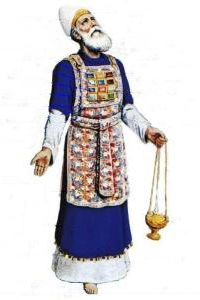
\includegraphics[width=50mm,scale=1.5]{Melchisedec.jpg}
\vspace{0.4in}

% Create a title for the document and write it in bold font
\LARGE{\textbf{\date}}
\linebreak

\vspace{0.5in}


\begin{flushleft}
\LARGE{1 Samuel\\}\vspace{0.25in}
\LARGE{Notes, Outlines, Comments}
\end{flushleft}

% write in large letters
%\large{Free webservices and apps}

% Skip some space
\vspace{0.6in}

%\large{Documentation}
% Skip some space

\bigskip

\normalsize{Xenia, Oh.\\}
\normalsize{created: \today}

% Skip some space
\vspace{1.3in}

\end{flushright}
% End the title page
\end{titlepage}

%\titlehttps://www.overleaf.com/project/60d732302fc633866943c9d2JE

\newpage 

\tableofcontents\hypertarget{TOC}{}
\listoffigures
\listoftables

\hyphenation{A-bim-e-lech bre-thren E-phra-im  Gib-e-o-nites Jer-u-sa-lem through-out Phil-i-stines The-o-phil-us Am-a-le-kites ven-geance Mesh-el-e-mi-ah onan-ism Phar-a-oh Py-thon thoughts grev-ous-ness Hach-a-liah adul-ter-er Shad-rach}

%\fcolorbox{black}{bone}{TEXT}
%%%%%%%%%%%%%%%%% EXTRA COLORS
%%%%%%%%%%%%%%%%% EXTRA COLORS
%%%%%%%%%%%%%%%%% EXTRA COLORS
\definecolor{champagne}{rgb}{0.97,0.91,0.81}
\definecolor{bone}{rgb}{0.89,0.85,0.79}

\definecolor{ForestGreen}{rgb}{0.00,0.29,0.098}
\definecolor{GIVING}{cmyk}{1,0.0,0.72,.1}

\definecolor{MLPE}{cmyk}{1,1,0,.45}
\definecolor{SOCCER}{cmyk}{.77, 0, .42, .49}
\definecolor{PAYBILL}{cmyk}{0,0.83,0.76,0.07}
\definecolor{SERMON}{cmyk}{.14,.9,0,.30} % aka seance \href{http://www.flatuicolorpicker.com/purple-cmyk-color-model/}{seance}
\definecolor{BIBLE}{cmyk}{0,.17,.74,.17}
\definecolor{WORKBLUE}{cmyk}{1, .5, 0, .6}
\definecolor{myOrange}{cmyk}{0, .4, .98, .03}
\definecolor{myTan}{cmyk}{0.0,.07,.17,.10}
\definecolor{myRed}{cmyk}{0,1,1,0}
\definecolor{myWhite}{cmyk}{0,0,0,0}
\definecolor{BLUESoD}{cmyk}{.97,.84,0,.04}
\definecolor{WHITE}{cmyk}{0,0,0,0}
\definecolor{OLDGOLD}{cmyk}{0.05,0.3,1.00,0}
\definecolor{CASTLETON}{cmyk}{1,0,0.31,0.66}
\definecolor{cadmiumgreen}{rgb}{0.0, 0.42, 0.24}
\definecolor{jungle}{rgb}{0.203,0.4882,0.1718}
\definecolor{MYGOLD}{rgb}{1,.84,0}

\definecolor{MYLIGHTGRAY}{rgb}{.85,.85,.85}

\definecolor{codegreen}{rgb}{0,0.6,0}
\definecolor{codegray}{rgb}{0.5,0.5,0.5}
\definecolor{codepurple}{rgb}{0.58,0,0.82}
\definecolor{backcolour}{rgb}{0.95,0.95,0.92}



\mdfdefinestyle{MyFrame}{%
    linecolor=blue,
    outerlinewidth=2pt,
    roundcorner=5pt,
    innertopmargin=\baselineskip,
    innerbottommargin=\baselineskip,
    innerrightmargin=10pt,
    innerleftmargin=10pt,
    backgroundcolor=gray!25!white}


\mdfdefinestyle{MyFrame2}{%
    linecolor=black,
    outerlinewidth=2pt,
    roundcorner=5pt,
    innertopmargin=\baselineskip,
    innerbottommargin=\baselineskip,
    innerrightmargin=10pt,
    innerleftmargin=10pt,
    backgroundcolor=yellow!25!white}



%\input{PFTTIS}
%\input{WFTTIS}
%\input{WFITV}


\chapter{1 Samuel 1}

\begin{figure}
  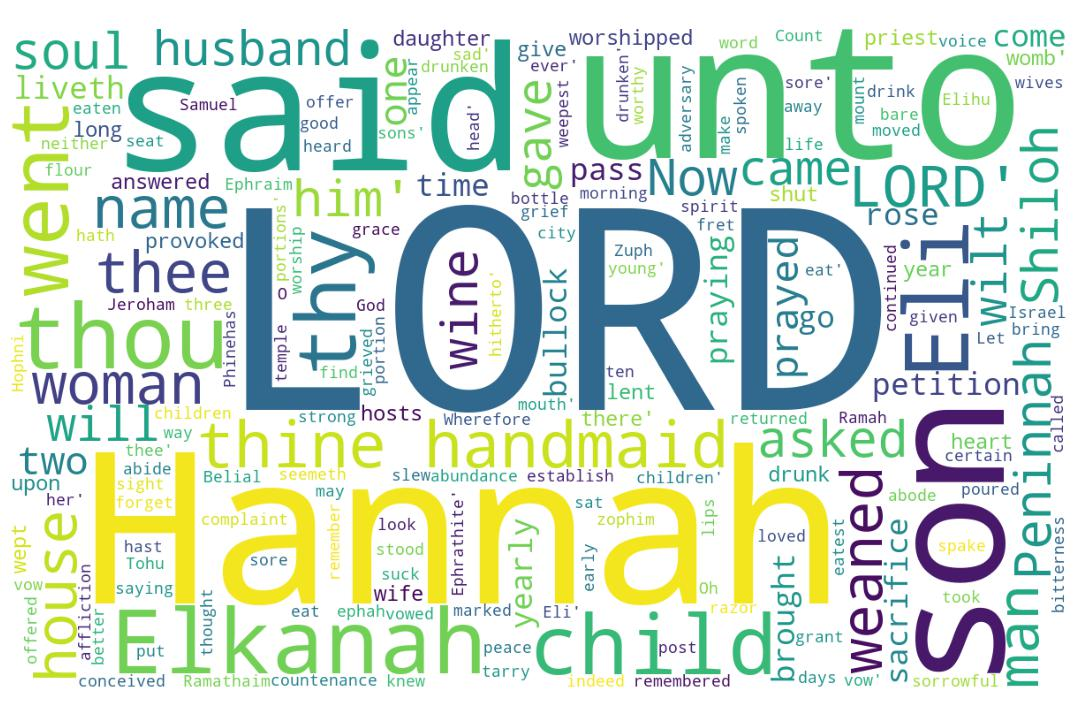
\includegraphics[width=\linewidth]{09OT-1Samuel/1Samuel1-WordCloud.jpg}
  \caption{1 Samuel 1 Word Cloud}
  \label{fig:1 Samuel 1 Word Cloud}
\end{figure}

\marginpar{\scriptsize \centering \fcolorbox{bone}{lime}{\textbf{A LENT SON}}\\ (1 Samuel 1:1-28) \begin{compactenum}[I.][8]
    \item A \textbf{Barren Woman}  \index[scripture]{1Samuel!1Sa 01:05}(1Sa 1:5)
    \item \textbf{Bitter \& Weeping}  \index[scripture]{1Samuel!1Sa 01:10}(1Sa 1:10)
    \item \textbf{Belial's Women}  \index[scripture]{1Samuel!1Sa 01:16}(1Sa 1:16)
    \item A \textbf{Baby Awaited}  \index[scripture]{1Samuel!1Sa 01:18}(1Sa 1:18)
    \item The \textbf{Boy Weaned}  \index[scripture]{1Samuel!1Sa 01:23}(1Sa 1:23)
    \item A \textbf{Blessed Woman}  \index[scripture]{1Samuel!1Sa 01:27}(1Sa 1:27)
    \item A \textbf{Boy Worshipping}  \index[scripture]{1Samuel!1Sa 01:28}(1Sa 1:28)
\end{compactenum}}






\footnote{\textcolor[cmyk]{0.99998,1,0,0}{\hyperlink{TOC}{Return to end of Table of Contents.}}}\footnote{\href{https://audiobible.com/bible/1_samuel_1.html}{\textcolor[cmyk]{0.99998,1,0,0}{1 Samuel 1 Audio}}}\textcolor[cmyk]{0.99998,1,0,0}{Now there was a certain man of Ramathaim-zophim, of mount Ephraim, and his name \emph{was} Elkanah, the son of Jeroham, the son of Elihu, the son of Tohu, the son of Zuph, an Ephrathite:}
[2] \textcolor[cmyk]{0.99998,1,0,0}{And he had two wives; the name of the one \emph{was} Hannah, and the name of the other Peninnah: and Peninnah had children, but Hannah had no children.}
[3] \textcolor[cmyk]{0.99998,1,0,0}{And this man went up out of his city yearly to worship and to sacrifice unto the LORD of hosts in Shiloh. And the two sons of Eli, Hophni and Phinehas, the priests of the LORD, \emph{were} there.}\\
\\
\P \textcolor[cmyk]{0.99998,1,0,0}{And when the time was that Elkanah offered, he gave to Peninnah his wife, and to all her sons and her daughters, portions:}
[5] \textcolor[cmyk]{0.99998,1,0,0}{But unto Hannah he gave a worthy portion; for he loved Hannah: but the LORD had \fcolorbox{bone}{lime}{shut up her womb}.}
[6] \textcolor[cmyk]{0.99998,1,0,0}{And her adversary also provoked her sore, for to make her fret, because the LORD had shut up her womb.}
[7] \textcolor[cmyk]{0.99998,1,0,0}{And \emph{as} he did so year by year, when she went up to the house of the LORD, so she provoked her; therefore she wept, and did not eat.}
[8] \textcolor[cmyk]{0.99998,1,0,0}{Then said Elkanah her husband to her, Hannah, why weepest thou? and why eatest thou not? and why is thy heart grieved? \emph{am} not I better to thee than ten sons?}\\
\\
\P \textcolor[cmyk]{0.99998,1,0,0}{So Hannah rose up after they had eaten in Shiloh, and after they had drunk. Now Eli the priest sat upon a seat by a post of the temple of the LORD.}
[10] \textcolor[cmyk]{0.99998,1,0,0}{And she \emph{was} \fcolorbox{bone}{lime}{in bitterness} of soul, and prayed unto the LORD, and wept sore.}
[11] \textcolor[cmyk]{0.99998,1,0,0}{And she vowed a vow, and said, O LORD of hosts, if thou wilt indeed look on the affliction of thine handmaid, and remember me, and not forget thine handmaid, but wilt give unto thine handmaid a man child, then I will give him unto the LORD all the days of his life, and there shall no razor come upon his head.}
[12] \textcolor[cmyk]{0.99998,1,0,0}{And it came to pass, as she continued praying before the LORD, that Eli marked her mouth.}
[13] \textcolor[cmyk]{0.99998,1,0,0}{Now Hannah, she spake in her heart; only her lips moved, but her voice was not heard: therefore Eli thought she had been drunken.}
[14] \textcolor[cmyk]{0.99998,1,0,0}{And Eli said unto her, How long wilt thou be drunken? put away thy wine from thee.}
[15] \textcolor[cmyk]{0.99998,1,0,0}{And Hannah answered and said, No, my lord, I \emph{am} a woman of a sorrowful spirit: I have drunk neither wine nor strong drink, but have poured out my soul before the LORD.}
[16] \textcolor[cmyk]{0.99998,1,0,0}{Count not thine handmaid for a \fcolorbox{bone}{lime}{daughter of Belial}: for out of the abundance of my complaint and grief have I spoken hitherto.}
[17] \textcolor[cmyk]{0.99998,1,0,0}{Then Eli answered and said, Go in peace: and the God of Israel grant \emph{thee} thy petition that thou hast asked of him.}
[18] \textcolor[cmyk]{0.99998,1,0,0}{And she said, Let thine handmaid find grace in thy sight. So the woman went her way, and did eat, and her countenance was no more \emph{sad}.}\\
\\
\P \textcolor[cmyk]{0.99998,1,0,0}{And they rose up in the morning early, and worshipped before the LORD, and returned, and came to their house to Ramah: and Elkanah knew Hannah his wife; and the LORD remembered her.}
[20] \textcolor[cmyk]{0.99998,1,0,0}{Wherefore it came to pass, when the time was come about after Hannah had conceived, that she bare a son, and called his name Samuel, \emph{saying}, Because I have asked him of the LORD.}
[21] \textcolor[cmyk]{0.99998,1,0,0}{And the man Elkanah, and all his house, went up to offer unto the LORD the yearly sacrifice, and his vow.}
[22] \textcolor[cmyk]{0.99998,1,0,0}{But Hannah went not up; for she said unto her husband, \emph{I} \emph{will} \emph{not} \emph{go} \emph{up} until the child be weaned, and \emph{then} I will bring him, that he may appear before the LORD, and there abide for ever.}
[23] \textcolor[cmyk]{0.99998,1,0,0}{And Elkanah her husband said unto her, Do what seemeth thee good; tarry until thou have \fcolorbox{bone}{lime}{weaned} him; only the LORD establish his word. So the woman abode, and gave her son suck until she \fcolorbox{bone}{lime}{weaned} him.}\\
\\
\P \textcolor[cmyk]{0.99998,1,0,0}{And when she had weaned him, she took him up with her, with three bullocks, and one ephah of flour, and a bottle of wine, and brought him unto the house of the LORD in Shiloh: and the child \emph{was} young.}
[25] \textcolor[cmyk]{0.99998,1,0,0}{And they slew a bullock, and brought the child to Eli.}
[26] \textcolor[cmyk]{0.99998,1,0,0}{And she said, Oh my lord, \emph{as} thy soul liveth, my lord, I \emph{am} the woman that stood by thee here, praying unto the LORD.}
[27] \textcolor[cmyk]{0.99998,1,0,0}{For this child I prayed; and the \fcolorbox{bone}{lime}{LORD hath given me} my petition which I asked of him:}
[28] \textcolor[cmyk]{0.99998,1,0,0}{Therefore also I have lent him to the LORD; as long as he liveth he shall be lent to the LORD. And \fcolorbox{bone}{lime}{he worshipped} the LORD there.}
\section{1 Samuel 1 Comments}


%\index[NWIV]{34!1Samuel!1Sa 1:1}\index[AWIP]{Now!1Samuel!1Sa 1:1}\index[AWIP]{there!1Samuel!1Sa 1:1}\index[AWIP]{was!1Samuel!1Sa 1:1}\index[AWIP]{a!1Samuel!1Sa 1:1}\index[AWIP]{certain!1Samuel!1Sa 1:1}\index[AWIP]{man!1Samuel!1Sa 1:1}\index[AWIP]{of!1Samuel!1Sa 1:1}\index[AWIP]{of!1Samuel!1Sa 1:1 (2)}\index[AWIP]{of!1Samuel!1Sa 1:1 (3)}\index[AWIP]{of!1Samuel!1Sa 1:1 (4)}\index[AWIP]{of!1Samuel!1Sa 1:1 (5)}\index[AWIP]{of!1Samuel!1Sa 1:1 (6)}\index[AWIP]{Ramathaim-zophim!1Samuel!1Sa 1:1}\index[AWIP]{mount!1Samuel!1Sa 1:1}\index[AWIP]{Ephraim!1Samuel!1Sa 1:1}\index[AWIP]{and!1Samuel!1Sa 1:1}\index[AWIP]{his!1Samuel!1Sa 1:1}\index[AWIP]{name!1Samuel!1Sa 1:1}\index[AWIP]{\emph{was}!1Samuel!1Sa 1:1}\index[AWIP]{Elkanah!1Samuel!1Sa 1:1}\index[AWIP]{the!1Samuel!1Sa 1:1}\index[AWIP]{the!1Samuel!1Sa 1:1 (2)}\index[AWIP]{the!1Samuel!1Sa 1:1 (3)}\index[AWIP]{the!1Samuel!1Sa 1:1 (4)}\index[AWIP]{son!1Samuel!1Sa 1:1}\index[AWIP]{son!1Samuel!1Sa 1:1 (2)}\index[AWIP]{son!1Samuel!1Sa 1:1 (3)}\index[AWIP]{son!1Samuel!1Sa 1:1 (4)}\index[AWIP]{Jeroham!1Samuel!1Sa 1:1}\index[AWIP]{Elihu!1Samuel!1Sa 1:1}\index[AWIP]{Tohu!1Samuel!1Sa 1:1}\index[AWIP]{Zuph!1Samuel!1Sa 1:1}\index[AWIP]{an!1Samuel!1Sa 1:1}\index[AWIP]{Ephrathite!1Samuel!1Sa 1:1}\index[AWIP]{\emph{was}!1Samuel!1Sa 1:1}

\index[NWIV]{28!1Samuel!1Sa 1:2}\index[AWIP]{And!1Samuel!1Sa 1:2}\index[AWIP]{he!1Samuel!1Sa 1:2}\index[AWIP]{had!1Samuel!1Sa 1:2}\index[AWIP]{had!1Samuel!1Sa 1:2 (2)}\index[AWIP]{had!1Samuel!1Sa 1:2 (3)}\index[AWIP]{two!1Samuel!1Sa 1:2}\index[AWIP]{wives!1Samuel!1Sa 1:2}\index[AWIP]{the!1Samuel!1Sa 1:2}\index[AWIP]{the!1Samuel!1Sa 1:2 (2)}\index[AWIP]{the!1Samuel!1Sa 1:2 (3)}\index[AWIP]{the!1Samuel!1Sa 1:2 (4)}\index[AWIP]{name!1Samuel!1Sa 1:2}\index[AWIP]{name!1Samuel!1Sa 1:2 (2)}\index[AWIP]{of!1Samuel!1Sa 1:2}\index[AWIP]{of!1Samuel!1Sa 1:2 (2)}\index[AWIP]{one!1Samuel!1Sa 1:2}\index[AWIP]{\emph{was}!1Samuel!1Sa 1:2}\index[AWIP]{Hannah!1Samuel!1Sa 1:2}\index[AWIP]{Hannah!1Samuel!1Sa 1:2 (2)}\index[AWIP]{and!1Samuel!1Sa 1:2}\index[AWIP]{and!1Samuel!1Sa 1:2 (2)}\index[AWIP]{other!1Samuel!1Sa 1:2}\index[AWIP]{Peninnah!1Samuel!1Sa 1:2}\index[AWIP]{Peninnah!1Samuel!1Sa 1:2 (2)}\index[AWIP]{children!1Samuel!1Sa 1:2}\index[AWIP]{children!1Samuel!1Sa 1:2 (2)}\index[AWIP]{but!1Samuel!1Sa 1:2}\index[AWIP]{no!1Samuel!1Sa 1:2}\index[AWIP]{\emph{was}!1Samuel!1Sa 1:2}

\index[NWIV]{38!1Samuel!1Sa 1:3}\index[AWIP]{And!1Samuel!1Sa 1:3}\index[AWIP]{And!1Samuel!1Sa 1:3 (2)}\index[AWIP]{this!1Samuel!1Sa 1:3}\index[AWIP]{man!1Samuel!1Sa 1:3}\index[AWIP]{went!1Samuel!1Sa 1:3}\index[AWIP]{up!1Samuel!1Sa 1:3}\index[AWIP]{out!1Samuel!1Sa 1:3}\index[AWIP]{of!1Samuel!1Sa 1:3}\index[AWIP]{of!1Samuel!1Sa 1:3 (2)}\index[AWIP]{of!1Samuel!1Sa 1:3 (3)}\index[AWIP]{of!1Samuel!1Sa 1:3 (4)}\index[AWIP]{his!1Samuel!1Sa 1:3}\index[AWIP]{city!1Samuel!1Sa 1:3}\index[AWIP]{yearly!1Samuel!1Sa 1:3}\index[AWIP]{to!1Samuel!1Sa 1:3}\index[AWIP]{to!1Samuel!1Sa 1:3 (2)}\index[AWIP]{worship!1Samuel!1Sa 1:3}\index[AWIP]{and!1Samuel!1Sa 1:3}\index[AWIP]{and!1Samuel!1Sa 1:3 (2)}\index[AWIP]{sacrifice!1Samuel!1Sa 1:3}\index[AWIP]{unto!1Samuel!1Sa 1:3}\index[AWIP]{the!1Samuel!1Sa 1:3}\index[AWIP]{the!1Samuel!1Sa 1:3 (2)}\index[AWIP]{the!1Samuel!1Sa 1:3 (3)}\index[AWIP]{the!1Samuel!1Sa 1:3 (4)}\index[AWIP]{LORD!1Samuel!1Sa 1:3}\index[AWIP]{LORD!1Samuel!1Sa 1:3 (2)}\index[AWIP]{hosts!1Samuel!1Sa 1:3}\index[AWIP]{in!1Samuel!1Sa 1:3}\index[AWIP]{Shiloh!1Samuel!1Sa 1:3}\index[AWIP]{two!1Samuel!1Sa 1:3}\index[AWIP]{sons!1Samuel!1Sa 1:3}\index[AWIP]{Eli!1Samuel!1Sa 1:3}\index[AWIP]{Hophni!1Samuel!1Sa 1:3}\index[AWIP]{Phinehas!1Samuel!1Sa 1:3}\index[AWIP]{priests!1Samuel!1Sa 1:3}\index[AWIP]{\emph{were}!1Samuel!1Sa 1:3}\index[AWIP]{there!1Samuel!1Sa 1:3}\index[AWIP]{\emph{were}!1Samuel!1Sa 1:3}

\index[NWIV]{23!1Samuel!1Sa 1:4}\index[AWIP]{And!1Samuel!1Sa 1:4}\index[AWIP]{when!1Samuel!1Sa 1:4}\index[AWIP]{the!1Samuel!1Sa 1:4}\index[AWIP]{time!1Samuel!1Sa 1:4}\index[AWIP]{was!1Samuel!1Sa 1:4}\index[AWIP]{that!1Samuel!1Sa 1:4}\index[AWIP]{Elkanah!1Samuel!1Sa 1:4}\index[AWIP]{offered!1Samuel!1Sa 1:4}\index[AWIP]{he!1Samuel!1Sa 1:4}\index[AWIP]{gave!1Samuel!1Sa 1:4}\index[AWIP]{to!1Samuel!1Sa 1:4}\index[AWIP]{to!1Samuel!1Sa 1:4 (2)}\index[AWIP]{Peninnah!1Samuel!1Sa 1:4}\index[AWIP]{his!1Samuel!1Sa 1:4}\index[AWIP]{wife!1Samuel!1Sa 1:4}\index[AWIP]{and!1Samuel!1Sa 1:4}\index[AWIP]{and!1Samuel!1Sa 1:4 (2)}\index[AWIP]{all!1Samuel!1Sa 1:4}\index[AWIP]{her!1Samuel!1Sa 1:4}\index[AWIP]{her!1Samuel!1Sa 1:4 (2)}\index[AWIP]{sons!1Samuel!1Sa 1:4}\index[AWIP]{daughters!1Samuel!1Sa 1:4}\index[AWIP]{portions!1Samuel!1Sa 1:4}

\index[NWIV]{20!1Samuel!1Sa 1:5}\index[AWIP]{But!1Samuel!1Sa 1:5}\index[AWIP]{unto!1Samuel!1Sa 1:5}\index[AWIP]{Hannah!1Samuel!1Sa 1:5}\index[AWIP]{Hannah!1Samuel!1Sa 1:5 (2)}\index[AWIP]{he!1Samuel!1Sa 1:5}\index[AWIP]{he!1Samuel!1Sa 1:5 (2)}\index[AWIP]{gave!1Samuel!1Sa 1:5}\index[AWIP]{a!1Samuel!1Sa 1:5}\index[AWIP]{worthy!1Samuel!1Sa 1:5}\index[AWIP]{portion!1Samuel!1Sa 1:5}\index[AWIP]{for!1Samuel!1Sa 1:5}\index[AWIP]{loved!1Samuel!1Sa 1:5}\index[AWIP]{but!1Samuel!1Sa 1:5}\index[AWIP]{the!1Samuel!1Sa 1:5}\index[AWIP]{LORD!1Samuel!1Sa 1:5}\index[AWIP]{had!1Samuel!1Sa 1:5}\index[AWIP]{shut!1Samuel!1Sa 1:5}\index[AWIP]{up!1Samuel!1Sa 1:5}\index[AWIP]{her!1Samuel!1Sa 1:5}\index[AWIP]{womb!1Samuel!1Sa 1:5}

\index[NWIV]{20!1Samuel!1Sa 1:6}\index[AWIP]{And!1Samuel!1Sa 1:6}\index[AWIP]{her!1Samuel!1Sa 1:6}\index[AWIP]{her!1Samuel!1Sa 1:6 (2)}\index[AWIP]{her!1Samuel!1Sa 1:6 (3)}\index[AWIP]{her!1Samuel!1Sa 1:6 (4)}\index[AWIP]{adversary!1Samuel!1Sa 1:6}\index[AWIP]{also!1Samuel!1Sa 1:6}\index[AWIP]{provoked!1Samuel!1Sa 1:6}\index[AWIP]{sore!1Samuel!1Sa 1:6}\index[AWIP]{for!1Samuel!1Sa 1:6}\index[AWIP]{to!1Samuel!1Sa 1:6}\index[AWIP]{make!1Samuel!1Sa 1:6}\index[AWIP]{fret!1Samuel!1Sa 1:6}\index[AWIP]{because!1Samuel!1Sa 1:6}\index[AWIP]{the!1Samuel!1Sa 1:6}\index[AWIP]{LORD!1Samuel!1Sa 1:6}\index[AWIP]{had!1Samuel!1Sa 1:6}\index[AWIP]{shut!1Samuel!1Sa 1:6}\index[AWIP]{up!1Samuel!1Sa 1:6}\index[AWIP]{womb!1Samuel!1Sa 1:6}

\index[NWIV]{29!1Samuel!1Sa 1:7}\index[AWIP]{And!1Samuel!1Sa 1:7}\index[AWIP]{\emph{as}!1Samuel!1Sa 1:7}\index[AWIP]{he!1Samuel!1Sa 1:7}\index[AWIP]{did!1Samuel!1Sa 1:7}\index[AWIP]{did!1Samuel!1Sa 1:7 (2)}\index[AWIP]{so!1Samuel!1Sa 1:7}\index[AWIP]{so!1Samuel!1Sa 1:7 (2)}\index[AWIP]{year!1Samuel!1Sa 1:7}\index[AWIP]{year!1Samuel!1Sa 1:7 (2)}\index[AWIP]{by!1Samuel!1Sa 1:7}\index[AWIP]{when!1Samuel!1Sa 1:7}\index[AWIP]{she!1Samuel!1Sa 1:7}\index[AWIP]{she!1Samuel!1Sa 1:7 (2)}\index[AWIP]{she!1Samuel!1Sa 1:7 (3)}\index[AWIP]{went!1Samuel!1Sa 1:7}\index[AWIP]{up!1Samuel!1Sa 1:7}\index[AWIP]{to!1Samuel!1Sa 1:7}\index[AWIP]{the!1Samuel!1Sa 1:7}\index[AWIP]{the!1Samuel!1Sa 1:7 (2)}\index[AWIP]{house!1Samuel!1Sa 1:7}\index[AWIP]{of!1Samuel!1Sa 1:7}\index[AWIP]{LORD!1Samuel!1Sa 1:7}\index[AWIP]{provoked!1Samuel!1Sa 1:7}\index[AWIP]{her!1Samuel!1Sa 1:7}\index[AWIP]{therefore!1Samuel!1Sa 1:7}\index[AWIP]{wept!1Samuel!1Sa 1:7}\index[AWIP]{and!1Samuel!1Sa 1:7}\index[AWIP]{not!1Samuel!1Sa 1:7}\index[AWIP]{eat!1Samuel!1Sa 1:7}\index[AWIP]{\emph{as}!1Samuel!1Sa 1:7}

\index[NWIV]{31!1Samuel!1Sa 1:8}\index[AWIP]{Then!1Samuel!1Sa 1:8}\index[AWIP]{said!1Samuel!1Sa 1:8}\index[AWIP]{Elkanah!1Samuel!1Sa 1:8}\index[AWIP]{her!1Samuel!1Sa 1:8}\index[AWIP]{her!1Samuel!1Sa 1:8 (2)}\index[AWIP]{husband!1Samuel!1Sa 1:8}\index[AWIP]{to!1Samuel!1Sa 1:8}\index[AWIP]{to!1Samuel!1Sa 1:8 (2)}\index[AWIP]{Hannah!1Samuel!1Sa 1:8}\index[AWIP]{why!1Samuel!1Sa 1:8}\index[AWIP]{why!1Samuel!1Sa 1:8 (2)}\index[AWIP]{why!1Samuel!1Sa 1:8 (3)}\index[AWIP]{weepest!1Samuel!1Sa 1:8}\index[AWIP]{thou?!1Samuel!1Sa 1:8}\index[AWIP]{and!1Samuel!1Sa 1:8}\index[AWIP]{and!1Samuel!1Sa 1:8 (2)}\index[AWIP]{eatest!1Samuel!1Sa 1:8}\index[AWIP]{thou!1Samuel!1Sa 1:8}\index[AWIP]{not?!1Samuel!1Sa 1:8}\index[AWIP]{is!1Samuel!1Sa 1:8}\index[AWIP]{thy!1Samuel!1Sa 1:8}\index[AWIP]{heart!1Samuel!1Sa 1:8}\index[AWIP]{grieved?!1Samuel!1Sa 1:8}\index[AWIP]{\emph{am}!1Samuel!1Sa 1:8}\index[AWIP]{not!1Samuel!1Sa 1:8}\index[AWIP]{I!1Samuel!1Sa 1:8}\index[AWIP]{better!1Samuel!1Sa 1:8}\index[AWIP]{thee!1Samuel!1Sa 1:8}\index[AWIP]{than!1Samuel!1Sa 1:8}\index[AWIP]{ten!1Samuel!1Sa 1:8}\index[AWIP]{sons?!1Samuel!1Sa 1:8}\index[AWIP]{\emph{am}!1Samuel!1Sa 1:8}

\index[NWIV]{32!1Samuel!1Sa 1:9}\index[AWIP]{So!1Samuel!1Sa 1:9}\index[AWIP]{Hannah!1Samuel!1Sa 1:9}\index[AWIP]{rose!1Samuel!1Sa 1:9}\index[AWIP]{up!1Samuel!1Sa 1:9}\index[AWIP]{after!1Samuel!1Sa 1:9}\index[AWIP]{after!1Samuel!1Sa 1:9 (2)}\index[AWIP]{they!1Samuel!1Sa 1:9}\index[AWIP]{they!1Samuel!1Sa 1:9 (2)}\index[AWIP]{had!1Samuel!1Sa 1:9}\index[AWIP]{had!1Samuel!1Sa 1:9 (2)}\index[AWIP]{eaten!1Samuel!1Sa 1:9}\index[AWIP]{in!1Samuel!1Sa 1:9}\index[AWIP]{Shiloh!1Samuel!1Sa 1:9}\index[AWIP]{and!1Samuel!1Sa 1:9}\index[AWIP]{drunk!1Samuel!1Sa 1:9}\index[AWIP]{Now!1Samuel!1Sa 1:9}\index[AWIP]{Eli!1Samuel!1Sa 1:9}\index[AWIP]{the!1Samuel!1Sa 1:9}\index[AWIP]{the!1Samuel!1Sa 1:9 (2)}\index[AWIP]{the!1Samuel!1Sa 1:9 (3)}\index[AWIP]{priest!1Samuel!1Sa 1:9}\index[AWIP]{sat!1Samuel!1Sa 1:9}\index[AWIP]{upon!1Samuel!1Sa 1:9}\index[AWIP]{a!1Samuel!1Sa 1:9}\index[AWIP]{a!1Samuel!1Sa 1:9 (2)}\index[AWIP]{seat!1Samuel!1Sa 1:9}\index[AWIP]{by!1Samuel!1Sa 1:9}\index[AWIP]{post!1Samuel!1Sa 1:9}\index[AWIP]{of!1Samuel!1Sa 1:9}\index[AWIP]{of!1Samuel!1Sa 1:9 (2)}\index[AWIP]{temple!1Samuel!1Sa 1:9}\index[AWIP]{LORD!1Samuel!1Sa 1:9}

\index[NWIV]{15!1Samuel!1Sa 1:10}\index[AWIP]{And!1Samuel!1Sa 1:10}\index[AWIP]{she!1Samuel!1Sa 1:10}\index[AWIP]{\emph{was}!1Samuel!1Sa 1:10}\index[AWIP]{in!1Samuel!1Sa 1:10}\index[AWIP]{bitterness!1Samuel!1Sa 1:10}\index[AWIP]{of!1Samuel!1Sa 1:10}\index[AWIP]{soul!1Samuel!1Sa 1:10}\index[AWIP]{and!1Samuel!1Sa 1:10}\index[AWIP]{and!1Samuel!1Sa 1:10 (2)}\index[AWIP]{prayed!1Samuel!1Sa 1:10}\index[AWIP]{unto!1Samuel!1Sa 1:10}\index[AWIP]{the!1Samuel!1Sa 1:10}\index[AWIP]{LORD!1Samuel!1Sa 1:10}\index[AWIP]{wept!1Samuel!1Sa 1:10}\index[AWIP]{sore!1Samuel!1Sa 1:10}\index[AWIP]{\emph{was}!1Samuel!1Sa 1:10}

\index[NWIV]{62!1Samuel!1Sa 1:11}\index[AWIP]{And!1Samuel!1Sa 1:11}\index[AWIP]{she!1Samuel!1Sa 1:11}\index[AWIP]{vowed!1Samuel!1Sa 1:11}\index[AWIP]{a!1Samuel!1Sa 1:11}\index[AWIP]{a!1Samuel!1Sa 1:11 (2)}\index[AWIP]{vow!1Samuel!1Sa 1:11}\index[AWIP]{and!1Samuel!1Sa 1:11}\index[AWIP]{and!1Samuel!1Sa 1:11 (2)}\index[AWIP]{and!1Samuel!1Sa 1:11 (3)}\index[AWIP]{and!1Samuel!1Sa 1:11 (4)}\index[AWIP]{said!1Samuel!1Sa 1:11}\index[AWIP]{O!1Samuel!1Sa 1:11}\index[AWIP]{LORD!1Samuel!1Sa 1:11}\index[AWIP]{LORD!1Samuel!1Sa 1:11 (2)}\index[AWIP]{of!1Samuel!1Sa 1:11}\index[AWIP]{of!1Samuel!1Sa 1:11 (2)}\index[AWIP]{of!1Samuel!1Sa 1:11 (3)}\index[AWIP]{hosts!1Samuel!1Sa 1:11}\index[AWIP]{if!1Samuel!1Sa 1:11}\index[AWIP]{thou!1Samuel!1Sa 1:11}\index[AWIP]{wilt!1Samuel!1Sa 1:11}\index[AWIP]{wilt!1Samuel!1Sa 1:11 (2)}\index[AWIP]{indeed!1Samuel!1Sa 1:11}\index[AWIP]{look!1Samuel!1Sa 1:11}\index[AWIP]{on!1Samuel!1Sa 1:11}\index[AWIP]{the!1Samuel!1Sa 1:11}\index[AWIP]{the!1Samuel!1Sa 1:11 (2)}\index[AWIP]{the!1Samuel!1Sa 1:11 (3)}\index[AWIP]{affliction!1Samuel!1Sa 1:11}\index[AWIP]{thine!1Samuel!1Sa 1:11}\index[AWIP]{thine!1Samuel!1Sa 1:11 (2)}\index[AWIP]{thine!1Samuel!1Sa 1:11 (3)}\index[AWIP]{handmaid!1Samuel!1Sa 1:11}\index[AWIP]{handmaid!1Samuel!1Sa 1:11 (2)}\index[AWIP]{handmaid!1Samuel!1Sa 1:11 (3)}\index[AWIP]{remember!1Samuel!1Sa 1:11}\index[AWIP]{me!1Samuel!1Sa 1:11}\index[AWIP]{not!1Samuel!1Sa 1:11}\index[AWIP]{forget!1Samuel!1Sa 1:11}\index[AWIP]{but!1Samuel!1Sa 1:11}\index[AWIP]{give!1Samuel!1Sa 1:11}\index[AWIP]{give!1Samuel!1Sa 1:11 (2)}\index[AWIP]{unto!1Samuel!1Sa 1:11}\index[AWIP]{unto!1Samuel!1Sa 1:11 (2)}\index[AWIP]{man!1Samuel!1Sa 1:11}\index[AWIP]{child!1Samuel!1Sa 1:11}\index[AWIP]{then!1Samuel!1Sa 1:11}\index[AWIP]{I!1Samuel!1Sa 1:11}\index[AWIP]{will!1Samuel!1Sa 1:11}\index[AWIP]{him!1Samuel!1Sa 1:11}\index[AWIP]{all!1Samuel!1Sa 1:11}\index[AWIP]{days!1Samuel!1Sa 1:11}\index[AWIP]{his!1Samuel!1Sa 1:11}\index[AWIP]{his!1Samuel!1Sa 1:11 (2)}\index[AWIP]{life!1Samuel!1Sa 1:11}\index[AWIP]{there!1Samuel!1Sa 1:11}\index[AWIP]{shall!1Samuel!1Sa 1:11}\index[AWIP]{no!1Samuel!1Sa 1:11}\index[AWIP]{razor!1Samuel!1Sa 1:11}\index[AWIP]{come!1Samuel!1Sa 1:11}\index[AWIP]{upon!1Samuel!1Sa 1:11}\index[AWIP]{head!1Samuel!1Sa 1:11}

\index[NWIV]{17!1Samuel!1Sa 1:12}\index[AWIP]{And!1Samuel!1Sa 1:12}\index[AWIP]{it!1Samuel!1Sa 1:12}\index[AWIP]{came!1Samuel!1Sa 1:12}\index[AWIP]{to!1Samuel!1Sa 1:12}\index[AWIP]{pass!1Samuel!1Sa 1:12}\index[AWIP]{as!1Samuel!1Sa 1:12}\index[AWIP]{she!1Samuel!1Sa 1:12}\index[AWIP]{continued!1Samuel!1Sa 1:12}\index[AWIP]{praying!1Samuel!1Sa 1:12}\index[AWIP]{before!1Samuel!1Sa 1:12}\index[AWIP]{the!1Samuel!1Sa 1:12}\index[AWIP]{LORD!1Samuel!1Sa 1:12}\index[AWIP]{that!1Samuel!1Sa 1:12}\index[AWIP]{Eli!1Samuel!1Sa 1:12}\index[AWIP]{marked!1Samuel!1Sa 1:12}\index[AWIP]{her!1Samuel!1Sa 1:12}\index[AWIP]{mouth!1Samuel!1Sa 1:12}

\index[NWIV]{24!1Samuel!1Sa 1:13}\index[AWIP]{Now!1Samuel!1Sa 1:13}\index[AWIP]{Hannah!1Samuel!1Sa 1:13}\index[AWIP]{she!1Samuel!1Sa 1:13}\index[AWIP]{she!1Samuel!1Sa 1:13 (2)}\index[AWIP]{spake!1Samuel!1Sa 1:13}\index[AWIP]{in!1Samuel!1Sa 1:13}\index[AWIP]{her!1Samuel!1Sa 1:13}\index[AWIP]{her!1Samuel!1Sa 1:13 (2)}\index[AWIP]{her!1Samuel!1Sa 1:13 (3)}\index[AWIP]{heart!1Samuel!1Sa 1:13}\index[AWIP]{only!1Samuel!1Sa 1:13}\index[AWIP]{lips!1Samuel!1Sa 1:13}\index[AWIP]{moved!1Samuel!1Sa 1:13}\index[AWIP]{but!1Samuel!1Sa 1:13}\index[AWIP]{voice!1Samuel!1Sa 1:13}\index[AWIP]{was!1Samuel!1Sa 1:13}\index[AWIP]{not!1Samuel!1Sa 1:13}\index[AWIP]{heard!1Samuel!1Sa 1:13}\index[AWIP]{therefore!1Samuel!1Sa 1:13}\index[AWIP]{Eli!1Samuel!1Sa 1:13}\index[AWIP]{thought!1Samuel!1Sa 1:13}\index[AWIP]{had!1Samuel!1Sa 1:13}\index[AWIP]{been!1Samuel!1Sa 1:13}\index[AWIP]{drunken!1Samuel!1Sa 1:13}

\index[NWIV]{17!1Samuel!1Sa 1:14}\index[AWIP]{And!1Samuel!1Sa 1:14}\index[AWIP]{Eli!1Samuel!1Sa 1:14}\index[AWIP]{said!1Samuel!1Sa 1:14}\index[AWIP]{unto!1Samuel!1Sa 1:14}\index[AWIP]{her!1Samuel!1Sa 1:14}\index[AWIP]{How!1Samuel!1Sa 1:14}\index[AWIP]{long!1Samuel!1Sa 1:14}\index[AWIP]{wilt!1Samuel!1Sa 1:14}\index[AWIP]{thou!1Samuel!1Sa 1:14}\index[AWIP]{be!1Samuel!1Sa 1:14}\index[AWIP]{drunken?!1Samuel!1Sa 1:14}\index[AWIP]{put!1Samuel!1Sa 1:14}\index[AWIP]{away!1Samuel!1Sa 1:14}\index[AWIP]{thy!1Samuel!1Sa 1:14}\index[AWIP]{wine!1Samuel!1Sa 1:14}\index[AWIP]{from!1Samuel!1Sa 1:14}\index[AWIP]{thee!1Samuel!1Sa 1:14}

\index[NWIV]{33!1Samuel!1Sa 1:15}\index[AWIP]{And!1Samuel!1Sa 1:15}\index[AWIP]{Hannah!1Samuel!1Sa 1:15}\index[AWIP]{answered!1Samuel!1Sa 1:15}\index[AWIP]{and!1Samuel!1Sa 1:15}\index[AWIP]{said!1Samuel!1Sa 1:15}\index[AWIP]{No!1Samuel!1Sa 1:15}\index[AWIP]{my!1Samuel!1Sa 1:15}\index[AWIP]{my!1Samuel!1Sa 1:15 (2)}\index[AWIP]{lord!1Samuel!1Sa 1:15}\index[AWIP]{I!1Samuel!1Sa 1:15}\index[AWIP]{I!1Samuel!1Sa 1:15 (2)}\index[AWIP]{\emph{am}!1Samuel!1Sa 1:15}\index[AWIP]{a!1Samuel!1Sa 1:15}\index[AWIP]{a!1Samuel!1Sa 1:15 (2)}\index[AWIP]{woman!1Samuel!1Sa 1:15}\index[AWIP]{of!1Samuel!1Sa 1:15}\index[AWIP]{sorrowful!1Samuel!1Sa 1:15}\index[AWIP]{spirit!1Samuel!1Sa 1:15}\index[AWIP]{have!1Samuel!1Sa 1:15}\index[AWIP]{have!1Samuel!1Sa 1:15 (2)}\index[AWIP]{drunk!1Samuel!1Sa 1:15}\index[AWIP]{neither!1Samuel!1Sa 1:15}\index[AWIP]{wine!1Samuel!1Sa 1:15}\index[AWIP]{nor!1Samuel!1Sa 1:15}\index[AWIP]{strong!1Samuel!1Sa 1:15}\index[AWIP]{drink!1Samuel!1Sa 1:15}\index[AWIP]{but!1Samuel!1Sa 1:15}\index[AWIP]{poured!1Samuel!1Sa 1:15}\index[AWIP]{out!1Samuel!1Sa 1:15}\index[AWIP]{soul!1Samuel!1Sa 1:15}\index[AWIP]{before!1Samuel!1Sa 1:15}\index[AWIP]{the!1Samuel!1Sa 1:15}\index[AWIP]{LORD!1Samuel!1Sa 1:15}\index[AWIP]{\emph{am}!1Samuel!1Sa 1:15}

\index[NWIV]{23!1Samuel!1Sa 1:16}\index[AWIP]{Count!1Samuel!1Sa 1:16}\index[AWIP]{not!1Samuel!1Sa 1:16}\index[AWIP]{thine!1Samuel!1Sa 1:16}\index[AWIP]{handmaid!1Samuel!1Sa 1:16}\index[AWIP]{for!1Samuel!1Sa 1:16}\index[AWIP]{for!1Samuel!1Sa 1:16 (2)}\index[AWIP]{a!1Samuel!1Sa 1:16}\index[AWIP]{daughter!1Samuel!1Sa 1:16}\index[AWIP]{of!1Samuel!1Sa 1:16}\index[AWIP]{of!1Samuel!1Sa 1:16 (2)}\index[AWIP]{of!1Samuel!1Sa 1:16 (3)}\index[AWIP]{Belial!1Samuel!1Sa 1:16}\index[AWIP]{out!1Samuel!1Sa 1:16}\index[AWIP]{the!1Samuel!1Sa 1:16}\index[AWIP]{abundance!1Samuel!1Sa 1:16}\index[AWIP]{my!1Samuel!1Sa 1:16}\index[AWIP]{complaint!1Samuel!1Sa 1:16}\index[AWIP]{and!1Samuel!1Sa 1:16}\index[AWIP]{grief!1Samuel!1Sa 1:16}\index[AWIP]{have!1Samuel!1Sa 1:16}\index[AWIP]{I!1Samuel!1Sa 1:16}\index[AWIP]{spoken!1Samuel!1Sa 1:16}\index[AWIP]{hitherto!1Samuel!1Sa 1:16}

\index[NWIV]{23!1Samuel!1Sa 1:17}\index[AWIP]{Then!1Samuel!1Sa 1:17}\index[AWIP]{Eli!1Samuel!1Sa 1:17}\index[AWIP]{answered!1Samuel!1Sa 1:17}\index[AWIP]{and!1Samuel!1Sa 1:17}\index[AWIP]{and!1Samuel!1Sa 1:17 (2)}\index[AWIP]{said!1Samuel!1Sa 1:17}\index[AWIP]{Go!1Samuel!1Sa 1:17}\index[AWIP]{in!1Samuel!1Sa 1:17}\index[AWIP]{peace!1Samuel!1Sa 1:17}\index[AWIP]{the!1Samuel!1Sa 1:17}\index[AWIP]{God!1Samuel!1Sa 1:17}\index[AWIP]{of!1Samuel!1Sa 1:17}\index[AWIP]{of!1Samuel!1Sa 1:17 (2)}\index[AWIP]{Israel!1Samuel!1Sa 1:17}\index[AWIP]{grant!1Samuel!1Sa 1:17}\index[AWIP]{\emph{thee}!1Samuel!1Sa 1:17}\index[AWIP]{thy!1Samuel!1Sa 1:17}\index[AWIP]{petition!1Samuel!1Sa 1:17}\index[AWIP]{that!1Samuel!1Sa 1:17}\index[AWIP]{thou!1Samuel!1Sa 1:17}\index[AWIP]{hast!1Samuel!1Sa 1:17}\index[AWIP]{asked!1Samuel!1Sa 1:17}\index[AWIP]{him!1Samuel!1Sa 1:17}\index[AWIP]{\emph{thee}!1Samuel!1Sa 1:17}

\index[NWIV]{27!1Samuel!1Sa 1:18}\index[AWIP]{And!1Samuel!1Sa 1:18}\index[AWIP]{she!1Samuel!1Sa 1:18}\index[AWIP]{said!1Samuel!1Sa 1:18}\index[AWIP]{Let!1Samuel!1Sa 1:18}\index[AWIP]{thine!1Samuel!1Sa 1:18}\index[AWIP]{handmaid!1Samuel!1Sa 1:18}\index[AWIP]{find!1Samuel!1Sa 1:18}\index[AWIP]{grace!1Samuel!1Sa 1:18}\index[AWIP]{in!1Samuel!1Sa 1:18}\index[AWIP]{thy!1Samuel!1Sa 1:18}\index[AWIP]{sight!1Samuel!1Sa 1:18}\index[AWIP]{So!1Samuel!1Sa 1:18}\index[AWIP]{the!1Samuel!1Sa 1:18}\index[AWIP]{woman!1Samuel!1Sa 1:18}\index[AWIP]{went!1Samuel!1Sa 1:18}\index[AWIP]{her!1Samuel!1Sa 1:18}\index[AWIP]{her!1Samuel!1Sa 1:18 (2)}\index[AWIP]{way!1Samuel!1Sa 1:18}\index[AWIP]{and!1Samuel!1Sa 1:18}\index[AWIP]{and!1Samuel!1Sa 1:18 (2)}\index[AWIP]{did!1Samuel!1Sa 1:18}\index[AWIP]{eat!1Samuel!1Sa 1:18}\index[AWIP]{countenance!1Samuel!1Sa 1:18}\index[AWIP]{was!1Samuel!1Sa 1:18}\index[AWIP]{no!1Samuel!1Sa 1:18}\index[AWIP]{more!1Samuel!1Sa 1:18}\index[AWIP]{\emph{sad}!1Samuel!1Sa 1:18}\index[AWIP]{\emph{sad}!1Samuel!1Sa 1:18}

\index[NWIV]{33!1Samuel!1Sa 1:19}\index[AWIP]{And!1Samuel!1Sa 1:19}\index[AWIP]{they!1Samuel!1Sa 1:19}\index[AWIP]{rose!1Samuel!1Sa 1:19}\index[AWIP]{up!1Samuel!1Sa 1:19}\index[AWIP]{in!1Samuel!1Sa 1:19}\index[AWIP]{the!1Samuel!1Sa 1:19}\index[AWIP]{the!1Samuel!1Sa 1:19 (2)}\index[AWIP]{the!1Samuel!1Sa 1:19 (3)}\index[AWIP]{morning!1Samuel!1Sa 1:19}\index[AWIP]{early!1Samuel!1Sa 1:19}\index[AWIP]{and!1Samuel!1Sa 1:19}\index[AWIP]{and!1Samuel!1Sa 1:19 (2)}\index[AWIP]{and!1Samuel!1Sa 1:19 (3)}\index[AWIP]{and!1Samuel!1Sa 1:19 (4)}\index[AWIP]{and!1Samuel!1Sa 1:19 (5)}\index[AWIP]{worshipped!1Samuel!1Sa 1:19}\index[AWIP]{before!1Samuel!1Sa 1:19}\index[AWIP]{LORD!1Samuel!1Sa 1:19}\index[AWIP]{LORD!1Samuel!1Sa 1:19 (2)}\index[AWIP]{returned!1Samuel!1Sa 1:19}\index[AWIP]{came!1Samuel!1Sa 1:19}\index[AWIP]{to!1Samuel!1Sa 1:19}\index[AWIP]{to!1Samuel!1Sa 1:19 (2)}\index[AWIP]{their!1Samuel!1Sa 1:19}\index[AWIP]{house!1Samuel!1Sa 1:19}\index[AWIP]{Ramah!1Samuel!1Sa 1:19}\index[AWIP]{Elkanah!1Samuel!1Sa 1:19}\index[AWIP]{knew!1Samuel!1Sa 1:19}\index[AWIP]{Hannah!1Samuel!1Sa 1:19}\index[AWIP]{his!1Samuel!1Sa 1:19}\index[AWIP]{wife!1Samuel!1Sa 1:19}\index[AWIP]{remembered!1Samuel!1Sa 1:19}\index[AWIP]{her!1Samuel!1Sa 1:19}

\index[NWIV]{34!1Samuel!1Sa 1:20}\index[AWIP]{Wherefore!1Samuel!1Sa 1:20}\index[AWIP]{it!1Samuel!1Sa 1:20}\index[AWIP]{came!1Samuel!1Sa 1:20}\index[AWIP]{to!1Samuel!1Sa 1:20}\index[AWIP]{pass!1Samuel!1Sa 1:20}\index[AWIP]{when!1Samuel!1Sa 1:20}\index[AWIP]{the!1Samuel!1Sa 1:20}\index[AWIP]{the!1Samuel!1Sa 1:20 (2)}\index[AWIP]{time!1Samuel!1Sa 1:20}\index[AWIP]{was!1Samuel!1Sa 1:20}\index[AWIP]{come!1Samuel!1Sa 1:20}\index[AWIP]{about!1Samuel!1Sa 1:20}\index[AWIP]{after!1Samuel!1Sa 1:20}\index[AWIP]{Hannah!1Samuel!1Sa 1:20}\index[AWIP]{had!1Samuel!1Sa 1:20}\index[AWIP]{conceived!1Samuel!1Sa 1:20}\index[AWIP]{that!1Samuel!1Sa 1:20}\index[AWIP]{she!1Samuel!1Sa 1:20}\index[AWIP]{bare!1Samuel!1Sa 1:20}\index[AWIP]{a!1Samuel!1Sa 1:20}\index[AWIP]{son!1Samuel!1Sa 1:20}\index[AWIP]{and!1Samuel!1Sa 1:20}\index[AWIP]{called!1Samuel!1Sa 1:20}\index[AWIP]{his!1Samuel!1Sa 1:20}\index[AWIP]{name!1Samuel!1Sa 1:20}\index[AWIP]{Samuel!1Samuel!1Sa 1:20}\index[AWIP]{\emph{saying}!1Samuel!1Sa 1:20}\index[AWIP]{Because!1Samuel!1Sa 1:20}\index[AWIP]{I!1Samuel!1Sa 1:20}\index[AWIP]{have!1Samuel!1Sa 1:20}\index[AWIP]{asked!1Samuel!1Sa 1:20}\index[AWIP]{him!1Samuel!1Sa 1:20}\index[AWIP]{of!1Samuel!1Sa 1:20}\index[AWIP]{LORD!1Samuel!1Sa 1:20}\index[AWIP]{\emph{saying}!1Samuel!1Sa 1:20}

\index[NWIV]{21!1Samuel!1Sa 1:21}\index[AWIP]{And!1Samuel!1Sa 1:21}\index[AWIP]{the!1Samuel!1Sa 1:21}\index[AWIP]{the!1Samuel!1Sa 1:21 (2)}\index[AWIP]{the!1Samuel!1Sa 1:21 (3)}\index[AWIP]{man!1Samuel!1Sa 1:21}\index[AWIP]{Elkanah!1Samuel!1Sa 1:21}\index[AWIP]{and!1Samuel!1Sa 1:21}\index[AWIP]{and!1Samuel!1Sa 1:21 (2)}\index[AWIP]{all!1Samuel!1Sa 1:21}\index[AWIP]{his!1Samuel!1Sa 1:21}\index[AWIP]{his!1Samuel!1Sa 1:21 (2)}\index[AWIP]{house!1Samuel!1Sa 1:21}\index[AWIP]{went!1Samuel!1Sa 1:21}\index[AWIP]{up!1Samuel!1Sa 1:21}\index[AWIP]{to!1Samuel!1Sa 1:21}\index[AWIP]{offer!1Samuel!1Sa 1:21}\index[AWIP]{unto!1Samuel!1Sa 1:21}\index[AWIP]{LORD!1Samuel!1Sa 1:21}\index[AWIP]{yearly!1Samuel!1Sa 1:21}\index[AWIP]{sacrifice!1Samuel!1Sa 1:21}\index[AWIP]{vow!1Samuel!1Sa 1:21}

\index[NWIV]{39!1Samuel!1Sa 1:22}\index[AWIP]{But!1Samuel!1Sa 1:22}\index[AWIP]{Hannah!1Samuel!1Sa 1:22}\index[AWIP]{went!1Samuel!1Sa 1:22}\index[AWIP]{not!1Samuel!1Sa 1:22}\index[AWIP]{up!1Samuel!1Sa 1:22}\index[AWIP]{for!1Samuel!1Sa 1:22}\index[AWIP]{for!1Samuel!1Sa 1:22 (2)}\index[AWIP]{she!1Samuel!1Sa 1:22}\index[AWIP]{said!1Samuel!1Sa 1:22}\index[AWIP]{unto!1Samuel!1Sa 1:22}\index[AWIP]{her!1Samuel!1Sa 1:22}\index[AWIP]{husband!1Samuel!1Sa 1:22}\index[AWIP]{\emph{I}!1Samuel!1Sa 1:22}\index[AWIP]{\emph{will}!1Samuel!1Sa 1:22}\index[AWIP]{\emph{not}!1Samuel!1Sa 1:22}\index[AWIP]{\emph{go}!1Samuel!1Sa 1:22}\index[AWIP]{\emph{up}!1Samuel!1Sa 1:22}\index[AWIP]{until!1Samuel!1Sa 1:22}\index[AWIP]{the!1Samuel!1Sa 1:22}\index[AWIP]{the!1Samuel!1Sa 1:22 (2)}\index[AWIP]{child!1Samuel!1Sa 1:22}\index[AWIP]{be!1Samuel!1Sa 1:22}\index[AWIP]{weaned!1Samuel!1Sa 1:22}\index[AWIP]{and!1Samuel!1Sa 1:22}\index[AWIP]{and!1Samuel!1Sa 1:22 (2)}\index[AWIP]{\emph{then}!1Samuel!1Sa 1:22}\index[AWIP]{I!1Samuel!1Sa 1:22}\index[AWIP]{will!1Samuel!1Sa 1:22}\index[AWIP]{bring!1Samuel!1Sa 1:22}\index[AWIP]{him!1Samuel!1Sa 1:22}\index[AWIP]{that!1Samuel!1Sa 1:22}\index[AWIP]{he!1Samuel!1Sa 1:22}\index[AWIP]{may!1Samuel!1Sa 1:22}\index[AWIP]{appear!1Samuel!1Sa 1:22}\index[AWIP]{before!1Samuel!1Sa 1:22}\index[AWIP]{LORD!1Samuel!1Sa 1:22}\index[AWIP]{there!1Samuel!1Sa 1:22}\index[AWIP]{abide!1Samuel!1Sa 1:22}\index[AWIP]{ever!1Samuel!1Sa 1:22}\index[AWIP]{\emph{I}!1Samuel!1Sa 1:22}\index[AWIP]{\emph{will}!1Samuel!1Sa 1:22}\index[AWIP]{\emph{not}!1Samuel!1Sa 1:22}\index[AWIP]{\emph{go}!1Samuel!1Sa 1:22}\index[AWIP]{\emph{up}!1Samuel!1Sa 1:22}\index[AWIP]{\emph{then}!1Samuel!1Sa 1:22}

\index[NWIV]{37!1Samuel!1Sa 1:23}\index[AWIP]{And!1Samuel!1Sa 1:23}\index[AWIP]{Elkanah!1Samuel!1Sa 1:23}\index[AWIP]{her!1Samuel!1Sa 1:23}\index[AWIP]{her!1Samuel!1Sa 1:23 (2)}\index[AWIP]{her!1Samuel!1Sa 1:23 (3)}\index[AWIP]{husband!1Samuel!1Sa 1:23}\index[AWIP]{said!1Samuel!1Sa 1:23}\index[AWIP]{unto!1Samuel!1Sa 1:23}\index[AWIP]{Do!1Samuel!1Sa 1:23}\index[AWIP]{what!1Samuel!1Sa 1:23}\index[AWIP]{seemeth!1Samuel!1Sa 1:23}\index[AWIP]{thee!1Samuel!1Sa 1:23}\index[AWIP]{good!1Samuel!1Sa 1:23}\index[AWIP]{tarry!1Samuel!1Sa 1:23}\index[AWIP]{until!1Samuel!1Sa 1:23}\index[AWIP]{until!1Samuel!1Sa 1:23 (2)}\index[AWIP]{thou!1Samuel!1Sa 1:23}\index[AWIP]{have!1Samuel!1Sa 1:23}\index[AWIP]{weaned!1Samuel!1Sa 1:23}\index[AWIP]{weaned!1Samuel!1Sa 1:23 (2)}\index[AWIP]{him!1Samuel!1Sa 1:23}\index[AWIP]{him!1Samuel!1Sa 1:23 (2)}\index[AWIP]{only!1Samuel!1Sa 1:23}\index[AWIP]{the!1Samuel!1Sa 1:23}\index[AWIP]{the!1Samuel!1Sa 1:23 (2)}\index[AWIP]{LORD!1Samuel!1Sa 1:23}\index[AWIP]{establish!1Samuel!1Sa 1:23}\index[AWIP]{his!1Samuel!1Sa 1:23}\index[AWIP]{word!1Samuel!1Sa 1:23}\index[AWIP]{So!1Samuel!1Sa 1:23}\index[AWIP]{woman!1Samuel!1Sa 1:23}\index[AWIP]{abode!1Samuel!1Sa 1:23}\index[AWIP]{and!1Samuel!1Sa 1:23}\index[AWIP]{gave!1Samuel!1Sa 1:23}\index[AWIP]{son!1Samuel!1Sa 1:23}\index[AWIP]{suck!1Samuel!1Sa 1:23}\index[AWIP]{she!1Samuel!1Sa 1:23}

\index[NWIV]{41!1Samuel!1Sa 1:24}\index[AWIP]{And!1Samuel!1Sa 1:24}\index[AWIP]{when!1Samuel!1Sa 1:24}\index[AWIP]{she!1Samuel!1Sa 1:24}\index[AWIP]{she!1Samuel!1Sa 1:24 (2)}\index[AWIP]{had!1Samuel!1Sa 1:24}\index[AWIP]{weaned!1Samuel!1Sa 1:24}\index[AWIP]{him!1Samuel!1Sa 1:24}\index[AWIP]{him!1Samuel!1Sa 1:24 (2)}\index[AWIP]{him!1Samuel!1Sa 1:24 (3)}\index[AWIP]{took!1Samuel!1Sa 1:24}\index[AWIP]{up!1Samuel!1Sa 1:24}\index[AWIP]{with!1Samuel!1Sa 1:24}\index[AWIP]{with!1Samuel!1Sa 1:24 (2)}\index[AWIP]{her!1Samuel!1Sa 1:24}\index[AWIP]{three!1Samuel!1Sa 1:24}\index[AWIP]{bullocks!1Samuel!1Sa 1:24}\index[AWIP]{and!1Samuel!1Sa 1:24}\index[AWIP]{and!1Samuel!1Sa 1:24 (2)}\index[AWIP]{and!1Samuel!1Sa 1:24 (3)}\index[AWIP]{and!1Samuel!1Sa 1:24 (4)}\index[AWIP]{one!1Samuel!1Sa 1:24}\index[AWIP]{ephah!1Samuel!1Sa 1:24}\index[AWIP]{of!1Samuel!1Sa 1:24}\index[AWIP]{of!1Samuel!1Sa 1:24 (2)}\index[AWIP]{of!1Samuel!1Sa 1:24 (3)}\index[AWIP]{flour!1Samuel!1Sa 1:24}\index[AWIP]{a!1Samuel!1Sa 1:24}\index[AWIP]{bottle!1Samuel!1Sa 1:24}\index[AWIP]{wine!1Samuel!1Sa 1:24}\index[AWIP]{brought!1Samuel!1Sa 1:24}\index[AWIP]{unto!1Samuel!1Sa 1:24}\index[AWIP]{the!1Samuel!1Sa 1:24}\index[AWIP]{the!1Samuel!1Sa 1:24 (2)}\index[AWIP]{the!1Samuel!1Sa 1:24 (3)}\index[AWIP]{house!1Samuel!1Sa 1:24}\index[AWIP]{LORD!1Samuel!1Sa 1:24}\index[AWIP]{in!1Samuel!1Sa 1:24}\index[AWIP]{Shiloh!1Samuel!1Sa 1:24}\index[AWIP]{child!1Samuel!1Sa 1:24}\index[AWIP]{\emph{was}!1Samuel!1Sa 1:24}\index[AWIP]{young!1Samuel!1Sa 1:24}\index[AWIP]{\emph{was}!1Samuel!1Sa 1:24}

\index[NWIV]{11!1Samuel!1Sa 1:25}\index[AWIP]{And!1Samuel!1Sa 1:25}\index[AWIP]{they!1Samuel!1Sa 1:25}\index[AWIP]{slew!1Samuel!1Sa 1:25}\index[AWIP]{a!1Samuel!1Sa 1:25}\index[AWIP]{bullock!1Samuel!1Sa 1:25}\index[AWIP]{and!1Samuel!1Sa 1:25}\index[AWIP]{brought!1Samuel!1Sa 1:25}\index[AWIP]{the!1Samuel!1Sa 1:25}\index[AWIP]{child!1Samuel!1Sa 1:25}\index[AWIP]{to!1Samuel!1Sa 1:25}\index[AWIP]{Eli!1Samuel!1Sa 1:25}

\index[NWIV]{25!1Samuel!1Sa 1:26}\index[AWIP]{And!1Samuel!1Sa 1:26}\index[AWIP]{she!1Samuel!1Sa 1:26}\index[AWIP]{said!1Samuel!1Sa 1:26}\index[AWIP]{Oh!1Samuel!1Sa 1:26}\index[AWIP]{my!1Samuel!1Sa 1:26}\index[AWIP]{my!1Samuel!1Sa 1:26 (2)}\index[AWIP]{lord!1Samuel!1Sa 1:26}\index[AWIP]{lord!1Samuel!1Sa 1:26 (2)}\index[AWIP]{\emph{as}!1Samuel!1Sa 1:26}\index[AWIP]{thy!1Samuel!1Sa 1:26}\index[AWIP]{soul!1Samuel!1Sa 1:26}\index[AWIP]{liveth!1Samuel!1Sa 1:26}\index[AWIP]{I!1Samuel!1Sa 1:26}\index[AWIP]{\emph{am}!1Samuel!1Sa 1:26}\index[AWIP]{the!1Samuel!1Sa 1:26}\index[AWIP]{the!1Samuel!1Sa 1:26 (2)}\index[AWIP]{woman!1Samuel!1Sa 1:26}\index[AWIP]{that!1Samuel!1Sa 1:26}\index[AWIP]{stood!1Samuel!1Sa 1:26}\index[AWIP]{by!1Samuel!1Sa 1:26}\index[AWIP]{thee!1Samuel!1Sa 1:26}\index[AWIP]{here!1Samuel!1Sa 1:26}\index[AWIP]{praying!1Samuel!1Sa 1:26}\index[AWIP]{unto!1Samuel!1Sa 1:26}\index[AWIP]{LORD!1Samuel!1Sa 1:26}\index[AWIP]{\emph{as}!1Samuel!1Sa 1:26}\index[AWIP]{\emph{am}!1Samuel!1Sa 1:26}

\index[NWIV]{18!1Samuel!1Sa 1:27}\index[AWIP]{For!1Samuel!1Sa 1:27}\index[AWIP]{this!1Samuel!1Sa 1:27}\index[AWIP]{child!1Samuel!1Sa 1:27}\index[AWIP]{I!1Samuel!1Sa 1:27}\index[AWIP]{I!1Samuel!1Sa 1:27 (2)}\index[AWIP]{prayed!1Samuel!1Sa 1:27}\index[AWIP]{and!1Samuel!1Sa 1:27}\index[AWIP]{the!1Samuel!1Sa 1:27}\index[AWIP]{LORD!1Samuel!1Sa 1:27}\index[AWIP]{hath!1Samuel!1Sa 1:27}\index[AWIP]{given!1Samuel!1Sa 1:27}\index[AWIP]{me!1Samuel!1Sa 1:27}\index[AWIP]{my!1Samuel!1Sa 1:27}\index[AWIP]{petition!1Samuel!1Sa 1:27}\index[AWIP]{which!1Samuel!1Sa 1:27}\index[AWIP]{asked!1Samuel!1Sa 1:27}\index[AWIP]{of!1Samuel!1Sa 1:27}\index[AWIP]{him!1Samuel!1Sa 1:27}

\index[NWIV]{27!1Samuel!1Sa 1:28}\index[AWIP]{Therefore!1Samuel!1Sa 1:28}\index[AWIP]{also!1Samuel!1Sa 1:28}\index[AWIP]{I!1Samuel!1Sa 1:28}\index[AWIP]{have!1Samuel!1Sa 1:28}\index[AWIP]{lent!1Samuel!1Sa 1:28}\index[AWIP]{lent!1Samuel!1Sa 1:28 (2)}\index[AWIP]{him!1Samuel!1Sa 1:28}\index[AWIP]{to!1Samuel!1Sa 1:28}\index[AWIP]{to!1Samuel!1Sa 1:28 (2)}\index[AWIP]{the!1Samuel!1Sa 1:28}\index[AWIP]{the!1Samuel!1Sa 1:28 (2)}\index[AWIP]{the!1Samuel!1Sa 1:28 (3)}\index[AWIP]{LORD!1Samuel!1Sa 1:28}\index[AWIP]{LORD!1Samuel!1Sa 1:28 (2)}\index[AWIP]{LORD!1Samuel!1Sa 1:28 (3)}\index[AWIP]{as!1Samuel!1Sa 1:28}\index[AWIP]{as!1Samuel!1Sa 1:28 (2)}\index[AWIP]{long!1Samuel!1Sa 1:28}\index[AWIP]{he!1Samuel!1Sa 1:28}\index[AWIP]{he!1Samuel!1Sa 1:28 (2)}\index[AWIP]{he!1Samuel!1Sa 1:28 (3)}\index[AWIP]{liveth!1Samuel!1Sa 1:28}\index[AWIP]{shall!1Samuel!1Sa 1:28}\index[AWIP]{be!1Samuel!1Sa 1:28}\index[AWIP]{And!1Samuel!1Sa 1:28}\index[AWIP]{worshipped!1Samuel!1Sa 1:28}\index[AWIP]{there!1Samuel!1Sa 1:28}


\section{1 Samuel 1 Outlines}

\subsection{My Outlines}

\subsubsection{A Lent Son}
\index[speaker]{Keith Anthony!1 Samuel 01 (A Lent Son)}
\index[series]{1 Samuel (Keith Anthony)!1 Samuel 01 (A Lent Son)}
\index[date]{2019/03/24!1 Samuel 01 (A Lent Son) (Keith Anthony)}

\begin{compactenum}[I.][7]
    \item A \textbf{Barren Woman}  \index[scripture]{1Samuel!1Sa 01:05}(1Sa 1:5)
    \item \textbf{Bitter \& Weeping}  \index[scripture]{1Samuel!1Sa 01:10}(1Sa 1:10)
    \item \textbf{Belial's Women}  \index[scripture]{1Samuel!1Sa 01:16}(1Sa 1:16)
    \item A \textbf{Baby Awaited}  \index[scripture]{1Samuel!1Sa 01:18}(1Sa 1:18)
    \item The \textbf{Boy Weaned}  \index[scripture]{1Samuel!1Sa 01:23}(1Sa 1:23)
    \item A \textbf{Blessed Woman}  \index[scripture]{1Samuel!1Sa 01:27}(1Sa 1:27)
    \item A \textbf{Boy Worshipping}  \index[scripture]{1Samuel!1Sa 01:28}(1Sa 1:28)
\end{compactenum}



\subsection{My Outlines from Others}

\subsubsection{A Son for Hannah}
\index[speaker]{Matt Bernsdorff!1 Samuel 01 (Samuel: A Yearning Heart \& A Baby’s Cry)}
\index[series]{1 Samuel (Matt Bernsdorff)!1 Samuel 01 (Samuel: A Yearning Heart \& A Baby’s Cry)}
\index[date]{unknown!1 Samuel 01 (Samuel: A Yearning Heart \& A Baby’s Cry) (Matt Bernsdorff)}
\textbf{Source: } Highlights Sunday School Curriculum
\begin{compactenum}[I.][7]
    \item The \textbf{Priest}  \index[scripture]{1Samuel!1Sa 01:03}(1Sa 1:3)
    \item A \textbf{Preference}  \index[scripture]{1Samuel!1Sa 01:05}(1Sa 1:5)
    \item The \textbf{Provocation} \index[scripture]{1Samuel!1Sa 01:06} \index[scripture]{1Samuel!1Sa 01:07}  (1Sa 1:6, 7)
    \item The \textbf{Passion} \index[scripture]{1Samuel!1Sa 01:07}(1Sa 1:7)
    \item The \textbf{Petition} \index[scripture]{1Samuel!1Sa 01:11}(1Sa 1:11
    \item The \textbf{Promise} \index[scripture]{1Samuel!1Sa 01:17}(1Sa 1:17)
    \item The \textbf{Presentation} \index[scripture]{1Samuel!1Sa 01:28}(1Sa 1:28)
\end{compactenum}

\subsubsection{God Answers Prayer}
\index[speaker]{Warren Wiersbe!1 Samuel 01 (God Answers Prayer)}
\index[series]{1 Samuel (Warren Wiersbe)!1 Samuel 01 (God Answers Prayer)}
\index[date]{unknown!1 Samuel 01 (God Answers Prayer) (Warren Wiersbe)}
\textbf{Source: }Wiersbe, BE Successful, Commentary on 1 Samuel
\begin{compactenum}[I.][7]
    \item A \textbf{Divided Home}  \index[scripture]{1Samuel!1Sa 01:01--08}(1Sa 1:1--8)
    \item A \textbf{Devout Prayer}  \index[scripture]{1Samuel!1Sa 01:09--19}(1Sa 1:9--18)
    \item A \textbf{Distinguished Son}  \index[scripture]{1Samuel!1Sa 01:19--28}(1Sa 1:19--28)
\end{compactenum}

%\\section{1 Samuel 1 Statistics}

%%%%%%%%%%%%%%%%%%%%%%%%%%%
%%%%% Word Statistics
%%%%%%%%%%%%%%%%%%%%%%%%%%


\normalsize



\subsection{Chapter Word Statistics}


%%%%%%%%%%
%%%%%%%%%%
 
\begin{center}
\begin{longtable}{l|c|c|c|c}
\caption[Stats for FirstSamuel 1]{Stats for FirstSamuel 1} \label{table:Stats for FirstSamuel 1} \\ 
\hline \multicolumn{1}{|c|}{\textbf{Verse(s)}} & \multicolumn{1}{|c|}{\textbf{Count}} & \multicolumn{1}{|c|}{\textbf{Unique}} & \multicolumn{1}{|c|}{\textbf{Italics}} & \multicolumn{1}{|c|}{\textbf{Uniq Italic}}  \\ \hline 
\endfirsthead
 
\multicolumn{5}{c}
{{\bfseries \tablename\ \thetable{} -- continued from previous page}} \\  
\hline \multicolumn{1}{|c|}{\textbf{Verse(s)}} & \multicolumn{1}{|c|}{\textbf{Count}} & \multicolumn{1}{|c|}{\textbf{Unique}} & \multicolumn{1}{|c|}{\textbf{Italics}} & \multicolumn{1}{|c|}{\textbf{Uniq Italic}}  \\ \hline 
\endhead
 
\hline \multicolumn{5}{|r|}{{Continued if needed}} \\ \hline
\endfoot 
1 & 34 & 23 & 1 & 1\\ \hline
2 & 28 & 17 & 1 & 1\\ \hline
3 & 38 & 28 & 1 & 1\\ \hline
4 & 23 & 20 & 0 & 0\\ \hline
5 & 20 & 18 & 0 & 0\\ \hline
6 & 20 & 17 & 0 & 0\\ \hline
7 & 29 & 23 & 1 & 1\\ \hline
8 & 31 & 24 & 1 & 1\\ \hline
9 & 32 & 25 & 0 & 0\\ \hline
10 & 15 & 14 & 1 & 1\\ \hline
11 & 62 & 45 & 0 & 0\\ \hline
12 & 17 & 17 & 0 & 0\\ \hline
13 & 24 & 21 & 0 & 0\\ \hline
14 & 17 & 17 & 0 & 0\\ \hline
15 & 33 & 29 & 1 & 1\\ \hline
16 & 23 & 20 & 0 & 0\\ \hline
17 & 23 & 21 & 1 & 1\\ \hline
18 & 27 & 25 & 1 & 1\\ \hline
19 & 33 & 25 & 0 & 0\\ \hline
20 & 34 & 33 & 1 & 1\\ \hline
21 & 21 & 17 & 0 & 0\\ \hline
22 & 39 & 36 & 6 & 6\\ \hline
23 & 37 & 31 & 0 & 0\\ \hline
24 & 41 & 30 & 1 & 1\\ \hline
25 & 11 & 11 & 0 & 0\\ \hline
26 & 25 & 22 & 2 & 2\\ \hline
27 & 18 & 17 & 0 & 0\\ \hline
28 & 27 & 18 & 0 & 0\\ \hline
\hline \hline
Total & 782 & 270 & 19 & 13



\end{longtable}
\end{center}

%%%%%%%%%%
%%%%%%%%%%
 
\subsection{Words by Frequency}

\begin{center}
\begin{longtable}{l|r}
\caption[Word Frequencies in FirstSamuel 1]{Word Frequencies in FirstSamuel 1} \label{table:WordsIn-FirstSamuel-1} \\ 
\hline \multicolumn{1}{|c|}{\textbf{Word}} & \multicolumn{1}{c|}{\textbf{Frequency}} \\ \hline 
\endfirsthead
 
\multicolumn{2}{c}
{{\bfseries \tablename\ \thetable{} -- continued from previous page}} \\ 
\hline \multicolumn{1}{|c|}{\textbf{Word}} & \multicolumn{1}{c|}{\textbf{Frequency}} \\ \hline 
\endhead
 
\hline \multicolumn{2}{|r|}{{Continued if needed}} \\ \hline
\endfoot
 
\hline \hline
\endlastfoot
the & 51 \\ \hline
and & 40 \\ \hline
of & 30 \\ \hline
LORD & 23 \\ \hline
her & 23 \\ \hline
And & 19 \\ \hline
to & 16 \\ \hline
she & 15 \\ \hline
a & 12 \\ \hline
Hannah & 11 \\ \hline
unto & 11 \\ \hline
I & 11 \\ \hline
him & 11 \\ \hline
his & 10 \\ \hline
had & 10 \\ \hline
he & 9 \\ \hline
up & 9 \\ \hline
said & 9 \\ \hline
in & 8 \\ \hline
Eli & 7 \\ \hline
not & 7 \\ \hline
Elkanah & 6 \\ \hline
son & 6 \\ \hline
that & 6 \\ \hline
for & 6 \\ \hline
thou & 6 \\ \hline
my & 6 \\ \hline
have & 6 \\ \hline
there & 5 \\ \hline
was & 5 \\ \hline
but & 5 \\ \hline
went & 5 \\ \hline
thy & 5 \\ \hline
thine & 5 \\ \hline
handmaid & 5 \\ \hline
child & 5 \\ \hline
man & 4 \\ \hline
name & 4 \\ \hline
\emph{was} & 4 \\ \hline
when & 4 \\ \hline
house & 4 \\ \hline
thee & 4 \\ \hline
they & 4 \\ \hline
before & 4 \\ \hline
woman & 4 \\ \hline
weaned & 4 \\ \hline
Now & 3 \\ \hline
Peninnah & 3 \\ \hline
no & 3 \\ \hline
out & 3 \\ \hline
Shiloh & 3 \\ \hline
sons & 3 \\ \hline
gave & 3 \\ \hline
all & 3 \\ \hline
did & 3 \\ \hline
by & 3 \\ \hline
husband & 3 \\ \hline
why & 3 \\ \hline
\emph{am} & 3 \\ \hline
So & 3 \\ \hline
after & 3 \\ \hline
soul & 3 \\ \hline
wilt & 3 \\ \hline
came & 3 \\ \hline
as & 3 \\ \hline
be & 3 \\ \hline
wine & 3 \\ \hline
lord & 3 \\ \hline
asked & 3 \\ \hline
until & 3 \\ \hline
two & 2 \\ \hline
one & 2 \\ \hline
children & 2 \\ \hline
this & 2 \\ \hline
yearly & 2 \\ \hline
sacrifice & 2 \\ \hline
hosts & 2 \\ \hline
time & 2 \\ \hline
wife & 2 \\ \hline
But & 2 \\ \hline
shut & 2 \\ \hline
womb & 2 \\ \hline
also & 2 \\ \hline
provoked & 2 \\ \hline
sore & 2 \\ \hline
\emph{as} & 2 \\ \hline
so & 2 \\ \hline
year & 2 \\ \hline
therefore & 2 \\ \hline
wept & 2 \\ \hline
eat & 2 \\ \hline
Then & 2 \\ \hline
heart & 2 \\ \hline
rose & 2 \\ \hline
drunk & 2 \\ \hline
upon & 2 \\ \hline
prayed & 2 \\ \hline
vow & 2 \\ \hline
me & 2 \\ \hline
give & 2 \\ \hline
will & 2 \\ \hline
shall & 2 \\ \hline
come & 2 \\ \hline
it & 2 \\ \hline
pass & 2 \\ \hline
praying & 2 \\ \hline
only & 2 \\ \hline
drunken & 2 \\ \hline
long & 2 \\ \hline
answered & 2 \\ \hline
petition & 2 \\ \hline
worshipped & 2 \\ \hline
with & 2 \\ \hline
brought & 2 \\ \hline
liveth & 2 \\ \hline
lent & 2 \\ \hline
certain & 1 \\ \hline
Ramathaim-zophim & 1 \\ \hline
mount & 1 \\ \hline
Ephraim & 1 \\ \hline
Jeroham & 1 \\ \hline
Elihu & 1 \\ \hline
Tohu & 1 \\ \hline
Zuph & 1 \\ \hline
an & 1 \\ \hline
Ephrathite & 1 \\ \hline
wives & 1 \\ \hline
other & 1 \\ \hline
city & 1 \\ \hline
worship & 1 \\ \hline
Hophni & 1 \\ \hline
Phinehas & 1 \\ \hline
priests & 1 \\ \hline
\emph{were} & 1 \\ \hline
offered & 1 \\ \hline
daughters & 1 \\ \hline
portions & 1 \\ \hline
worthy & 1 \\ \hline
portion & 1 \\ \hline
loved & 1 \\ \hline
adversary & 1 \\ \hline
make & 1 \\ \hline
fret & 1 \\ \hline
because & 1 \\ \hline
weepest & 1 \\ \hline
eatest & 1 \\ \hline
is & 1 \\ \hline
grieved & 1 \\ \hline
better & 1 \\ \hline
than & 1 \\ \hline
ten & 1 \\ \hline
eaten & 1 \\ \hline
priest & 1 \\ \hline
sat & 1 \\ \hline
seat & 1 \\ \hline
post & 1 \\ \hline
temple & 1 \\ \hline
bitterness & 1 \\ \hline
vowed & 1 \\ \hline
O & 1 \\ \hline
if & 1 \\ \hline
indeed & 1 \\ \hline
look & 1 \\ \hline
on & 1 \\ \hline
affliction & 1 \\ \hline
remember & 1 \\ \hline
forget & 1 \\ \hline
then & 1 \\ \hline
days & 1 \\ \hline
life & 1 \\ \hline
razor & 1 \\ \hline
head & 1 \\ \hline
continued & 1 \\ \hline
marked & 1 \\ \hline
mouth & 1 \\ \hline
spake & 1 \\ \hline
lips & 1 \\ \hline
moved & 1 \\ \hline
voice & 1 \\ \hline
heard & 1 \\ \hline
thought & 1 \\ \hline
been & 1 \\ \hline
How & 1 \\ \hline
put & 1 \\ \hline
away & 1 \\ \hline
from & 1 \\ \hline
No & 1 \\ \hline
sorrowful & 1 \\ \hline
spirit & 1 \\ \hline
neither & 1 \\ \hline
nor & 1 \\ \hline
strong & 1 \\ \hline
drink & 1 \\ \hline
poured & 1 \\ \hline
Count & 1 \\ \hline
daughter & 1 \\ \hline
Belial & 1 \\ \hline
abundance & 1 \\ \hline
complaint & 1 \\ \hline
grief & 1 \\ \hline
spoken & 1 \\ \hline
hitherto & 1 \\ \hline
Go & 1 \\ \hline
peace & 1 \\ \hline
God & 1 \\ \hline
Israel & 1 \\ \hline
grant & 1 \\ \hline
\emph{thee} & 1 \\ \hline
hast & 1 \\ \hline
Let & 1 \\ \hline
find & 1 \\ \hline
grace & 1 \\ \hline
sight & 1 \\ \hline
way & 1 \\ \hline
countenance & 1 \\ \hline
more & 1 \\ \hline
\emph{sad} & 1 \\ \hline
morning & 1 \\ \hline
early & 1 \\ \hline
returned & 1 \\ \hline
their & 1 \\ \hline
Ramah & 1 \\ \hline
knew & 1 \\ \hline
remembered & 1 \\ \hline
Wherefore & 1 \\ \hline
about & 1 \\ \hline
conceived & 1 \\ \hline
bare & 1 \\ \hline
called & 1 \\ \hline
Samuel & 1 \\ \hline
\emph{saying} & 1 \\ \hline
Because & 1 \\ \hline
offer & 1 \\ \hline
\emph{I} & 1 \\ \hline
\emph{will} & 1 \\ \hline
\emph{not} & 1 \\ \hline
\emph{go} & 1 \\ \hline
\emph{up} & 1 \\ \hline
\emph{then} & 1 \\ \hline
bring & 1 \\ \hline
may & 1 \\ \hline
appear & 1 \\ \hline
abide & 1 \\ \hline
ever & 1 \\ \hline
Do & 1 \\ \hline
what & 1 \\ \hline
seemeth & 1 \\ \hline
good & 1 \\ \hline
tarry & 1 \\ \hline
establish & 1 \\ \hline
word & 1 \\ \hline
abode & 1 \\ \hline
suck & 1 \\ \hline
took & 1 \\ \hline
three & 1 \\ \hline
bullocks & 1 \\ \hline
ephah & 1 \\ \hline
flour & 1 \\ \hline
bottle & 1 \\ \hline
young & 1 \\ \hline
slew & 1 \\ \hline
bullock & 1 \\ \hline
Oh & 1 \\ \hline
stood & 1 \\ \hline
here & 1 \\ \hline
For & 1 \\ \hline
hath & 1 \\ \hline
given & 1 \\ \hline
which & 1 \\ \hline
Therefore & 1 \\ \hline
\end{longtable}
\end{center}



\normalsize



\subsection{Words Alphabetically}

\begin{center}
\begin{longtable}{l|r}
\caption[Word Alphabetically in FirstSamuel 1]{Word Alphabetically in FirstSamuel 1} \label{table:WordsIn-FirstSamuel-1} \\ 
\hline \multicolumn{1}{|c|}{\textbf{Word}} & \multicolumn{1}{c|}{\textbf{Frequency}} \\ \hline 
\endfirsthead
 
\multicolumn{2}{c}
{{\bfseries \tablename\ \thetable{} -- continued from previous page}} \\ 
\hline \multicolumn{1}{|c|}{\textbf{Word}} & \multicolumn{1}{c|}{\textbf{Frequency}} \\ \hline 
\endhead
 
\hline \multicolumn{2}{|r|}{{Continued if needed}} \\ \hline
\endfoot
 
\hline \hline
\endlastfoot
And & 19 \\ \hline
Because & 1 \\ \hline
Belial & 1 \\ \hline
But & 2 \\ \hline
Count & 1 \\ \hline
Do & 1 \\ \hline
Eli & 7 \\ \hline
Elihu & 1 \\ \hline
Elkanah & 6 \\ \hline
Ephraim & 1 \\ \hline
Ephrathite & 1 \\ \hline
For & 1 \\ \hline
Go & 1 \\ \hline
God & 1 \\ \hline
Hannah & 11 \\ \hline
Hophni & 1 \\ \hline
How & 1 \\ \hline
I & 11 \\ \hline
Israel & 1 \\ \hline
Jeroham & 1 \\ \hline
LORD & 23 \\ \hline
Let & 1 \\ \hline
No & 1 \\ \hline
Now & 3 \\ \hline
O & 1 \\ \hline
Oh & 1 \\ \hline
Peninnah & 3 \\ \hline
Phinehas & 1 \\ \hline
Ramah & 1 \\ \hline
Ramathaim-zophim & 1 \\ \hline
Samuel & 1 \\ \hline
Shiloh & 3 \\ \hline
So & 3 \\ \hline
Then & 2 \\ \hline
Therefore & 1 \\ \hline
Tohu & 1 \\ \hline
Wherefore & 1 \\ \hline
Zuph & 1 \\ \hline
\emph{I} & 1 \\ \hline
\emph{am} & 3 \\ \hline
\emph{as} & 2 \\ \hline
\emph{go} & 1 \\ \hline
\emph{not} & 1 \\ \hline
\emph{sad} & 1 \\ \hline
\emph{saying} & 1 \\ \hline
\emph{thee} & 1 \\ \hline
\emph{then} & 1 \\ \hline
\emph{up} & 1 \\ \hline
\emph{was} & 4 \\ \hline
\emph{were} & 1 \\ \hline
\emph{will} & 1 \\ \hline
a & 12 \\ \hline
abide & 1 \\ \hline
abode & 1 \\ \hline
about & 1 \\ \hline
abundance & 1 \\ \hline
adversary & 1 \\ \hline
affliction & 1 \\ \hline
after & 3 \\ \hline
all & 3 \\ \hline
also & 2 \\ \hline
an & 1 \\ \hline
and & 40 \\ \hline
answered & 2 \\ \hline
appear & 1 \\ \hline
as & 3 \\ \hline
asked & 3 \\ \hline
away & 1 \\ \hline
bare & 1 \\ \hline
be & 3 \\ \hline
because & 1 \\ \hline
been & 1 \\ \hline
before & 4 \\ \hline
better & 1 \\ \hline
bitterness & 1 \\ \hline
bottle & 1 \\ \hline
bring & 1 \\ \hline
brought & 2 \\ \hline
bullock & 1 \\ \hline
bullocks & 1 \\ \hline
but & 5 \\ \hline
by & 3 \\ \hline
called & 1 \\ \hline
came & 3 \\ \hline
certain & 1 \\ \hline
child & 5 \\ \hline
children & 2 \\ \hline
city & 1 \\ \hline
come & 2 \\ \hline
complaint & 1 \\ \hline
conceived & 1 \\ \hline
continued & 1 \\ \hline
countenance & 1 \\ \hline
daughter & 1 \\ \hline
daughters & 1 \\ \hline
days & 1 \\ \hline
did & 3 \\ \hline
drink & 1 \\ \hline
drunk & 2 \\ \hline
drunken & 2 \\ \hline
early & 1 \\ \hline
eat & 2 \\ \hline
eaten & 1 \\ \hline
eatest & 1 \\ \hline
ephah & 1 \\ \hline
establish & 1 \\ \hline
ever & 1 \\ \hline
find & 1 \\ \hline
flour & 1 \\ \hline
for & 6 \\ \hline
forget & 1 \\ \hline
fret & 1 \\ \hline
from & 1 \\ \hline
gave & 3 \\ \hline
give & 2 \\ \hline
given & 1 \\ \hline
good & 1 \\ \hline
grace & 1 \\ \hline
grant & 1 \\ \hline
grief & 1 \\ \hline
grieved & 1 \\ \hline
had & 10 \\ \hline
handmaid & 5 \\ \hline
hast & 1 \\ \hline
hath & 1 \\ \hline
have & 6 \\ \hline
he & 9 \\ \hline
head & 1 \\ \hline
heard & 1 \\ \hline
heart & 2 \\ \hline
her & 23 \\ \hline
here & 1 \\ \hline
him & 11 \\ \hline
his & 10 \\ \hline
hitherto & 1 \\ \hline
hosts & 2 \\ \hline
house & 4 \\ \hline
husband & 3 \\ \hline
if & 1 \\ \hline
in & 8 \\ \hline
indeed & 1 \\ \hline
is & 1 \\ \hline
it & 2 \\ \hline
knew & 1 \\ \hline
lent & 2 \\ \hline
life & 1 \\ \hline
lips & 1 \\ \hline
liveth & 2 \\ \hline
long & 2 \\ \hline
look & 1 \\ \hline
lord & 3 \\ \hline
loved & 1 \\ \hline
make & 1 \\ \hline
man & 4 \\ \hline
marked & 1 \\ \hline
may & 1 \\ \hline
me & 2 \\ \hline
more & 1 \\ \hline
morning & 1 \\ \hline
mount & 1 \\ \hline
mouth & 1 \\ \hline
moved & 1 \\ \hline
my & 6 \\ \hline
name & 4 \\ \hline
neither & 1 \\ \hline
no & 3 \\ \hline
nor & 1 \\ \hline
not & 7 \\ \hline
of & 30 \\ \hline
offer & 1 \\ \hline
offered & 1 \\ \hline
on & 1 \\ \hline
one & 2 \\ \hline
only & 2 \\ \hline
other & 1 \\ \hline
out & 3 \\ \hline
pass & 2 \\ \hline
peace & 1 \\ \hline
petition & 2 \\ \hline
portion & 1 \\ \hline
portions & 1 \\ \hline
post & 1 \\ \hline
poured & 1 \\ \hline
prayed & 2 \\ \hline
praying & 2 \\ \hline
priest & 1 \\ \hline
priests & 1 \\ \hline
provoked & 2 \\ \hline
put & 1 \\ \hline
razor & 1 \\ \hline
remember & 1 \\ \hline
remembered & 1 \\ \hline
returned & 1 \\ \hline
rose & 2 \\ \hline
sacrifice & 2 \\ \hline
said & 9 \\ \hline
sat & 1 \\ \hline
seat & 1 \\ \hline
seemeth & 1 \\ \hline
shall & 2 \\ \hline
she & 15 \\ \hline
shut & 2 \\ \hline
sight & 1 \\ \hline
slew & 1 \\ \hline
so & 2 \\ \hline
son & 6 \\ \hline
sons & 3 \\ \hline
sore & 2 \\ \hline
sorrowful & 1 \\ \hline
soul & 3 \\ \hline
spake & 1 \\ \hline
spirit & 1 \\ \hline
spoken & 1 \\ \hline
stood & 1 \\ \hline
strong & 1 \\ \hline
suck & 1 \\ \hline
tarry & 1 \\ \hline
temple & 1 \\ \hline
ten & 1 \\ \hline
than & 1 \\ \hline
that & 6 \\ \hline
the & 51 \\ \hline
thee & 4 \\ \hline
their & 1 \\ \hline
then & 1 \\ \hline
there & 5 \\ \hline
therefore & 2 \\ \hline
they & 4 \\ \hline
thine & 5 \\ \hline
this & 2 \\ \hline
thou & 6 \\ \hline
thought & 1 \\ \hline
three & 1 \\ \hline
thy & 5 \\ \hline
time & 2 \\ \hline
to & 16 \\ \hline
took & 1 \\ \hline
two & 2 \\ \hline
until & 3 \\ \hline
unto & 11 \\ \hline
up & 9 \\ \hline
upon & 2 \\ \hline
voice & 1 \\ \hline
vow & 2 \\ \hline
vowed & 1 \\ \hline
was & 5 \\ \hline
way & 1 \\ \hline
weaned & 4 \\ \hline
weepest & 1 \\ \hline
went & 5 \\ \hline
wept & 2 \\ \hline
what & 1 \\ \hline
when & 4 \\ \hline
which & 1 \\ \hline
why & 3 \\ \hline
wife & 2 \\ \hline
will & 2 \\ \hline
wilt & 3 \\ \hline
wine & 3 \\ \hline
with & 2 \\ \hline
wives & 1 \\ \hline
woman & 4 \\ \hline
womb & 2 \\ \hline
word & 1 \\ \hline
worship & 1 \\ \hline
worshipped & 2 \\ \hline
worthy & 1 \\ \hline
year & 2 \\ \hline
yearly & 2 \\ \hline
young & 1 \\ \hline
\end{longtable}
\end{center}



\normalsize



\subsection{Word Lengths in Chapter}
\normalsize
\begin{longtable}{l|p{3.75in}}
\caption[Words by Length in FirstSamuel 1]{Words by Length in FirstSamuel 1} \label{table:WordsIn-FirstSamuel-1} \\ 
\hline \multicolumn{1}{|c|}{\textbf{Length}} & \multicolumn{1}{c|}{\textbf{Words}} \\ \hline 
\endfirsthead
 
\multicolumn{2}{c}
{{\bfseries \tablename\ \thetable{} -- continued from previous page}} \\ 
\hline \multicolumn{1}{|c|}{\textbf{Length}} & \multicolumn{1}{c|}{\textbf{Words}} \\ \hline 
\endhead
 
\hline \multicolumn{2}{|r|}{{Continued if needed}} \\ \hline
\endfoot
 
\hline \hline
\endlastfoot
1 & a, I, O, \emph{I} \\ \hline
2 & of, an, he, no, up, to, in, \emph{as}, so, by, is, \emph{am}, So, if, on, me, it, as, be, No, my, Go, \emph{go}, \emph{up}, Do, Oh \\ \hline
3 & Now, was, man, and, his, \emph{was}, the, son, And, had, two, one, but, out, Eli, all, her, But, for, did, she, not, eat, why, thy, ten, sat, vow, him, How, put, nor, God, Let, way, \emph{sad}, \emph{not}, may, For \\ \hline
4 & name, Tohu, Zuph, this, went, city, unto, LORD, sons, \emph{were}, when, time, that, gave, wife, shut, womb, also, sore, make, fret, year, wept, Then, said, thou, thee, than, rose, they, upon, seat, post, soul, wilt, look, give, then, will, days, life, come, head, came, pass, only, lips, been, long, away, wine, from, lord, have, \emph{thee}, hast, find, more, knew, bare, \emph{will}, \emph{then}, ever, what, good, word, suck, took, with, slew, here, hath, lent \\ \hline
5 & there, mount, Elihu, wives, other, hosts, loved, house, heart, after, eaten, drunk, vowed, thine, child, shall, razor, mouth, spake, moved, voice, heard, woman, drink, Count, grief, peace, grant, asked, grace, sight, early, their, Ramah, about, offer, until, bring, abide, tarry, abode, three, ephah, flour, young, stood, given, which \\ \hline
6 & Hannah, yearly, Shiloh, Hophni, worthy, eatest, better, priest, temple, prayed, indeed, forget, before, marked, spirit, strong, poured, Belial, spoken, Israel, called, Samuel, \emph{saying}, weaned, appear, bottle, liveth \\ \hline
7 & certain, Ephraim, Elkanah, Jeroham, worship, priests, offered, portion, because, husband, weepest, grieved, praying, thought, drunken, neither, morning, Because, seemeth, brought, bullock \\ \hline
8 & Peninnah, children, Phinehas, portions, provoked, handmaid, remember, answered, daughter, hitherto, petition, returned, bullocks \\ \hline
9 & sacrifice, daughters, adversary, therefore, continued, sorrowful, abundance, complaint, Wherefore, conceived, establish, Therefore \\ \hline
10 & Ephrathite, bitterness, affliction, worshipped, remembered \\ \hline
11 & countenance \\ \hline
16 & Ramathaim-zophim \\ \hline
\end{longtable}






%%%%%%%%%%
%%%%%%%%%%
 



%%%%%%%%%%
%%%%%%%%%%
\subsection{Verses with 18 Words in Chapter}
\normalsize
\begin{longtable}{l|p{3.75in}}
\caption[Verses with 18 Words  in FirstSamuel 1]{Verses with 18 Words  in FirstSamuel 1} \label{table:Verses with 18 Words in-FirstSamuel-1} \\ 
\hline \multicolumn{1}{|c|}{\textbf{Reference}} & \multicolumn{1}{c|}{\textbf{Verse}} \\ \hline 
\endfirsthead
 
\multicolumn{2}{c}
{{\bfseries \tablename\ \thetable{} -- continued from previous page}} \\ 
\hline \multicolumn{1}{|c|}{\textbf{Reference}} & \multicolumn{1}{c|}{\textbf{Verse}} \\ \hline 
\endhead
 
\hline \multicolumn{2}{|r|}{{Continued if needed}} \\ \hline
\endfoot
 
\hline \hline
\endlastfoot
1Samuel 01:27 & For this child I prayed; and the LORD hath given me my petition which I asked of him: \\ \hline
\end{longtable}






%%%%%%%%%%
%%%%%%%%%%
\subsection{1 Samuel 1 Repeated Phrases}


%%%%%%%%%%
%%%%%%%%%%
\normalsize
 
\begin{center}
\begin{longtable}{|p{3.0in}|p{0.5in}|}
\caption[1 Samuel 1 Repeated Phrases]{1 Samuel 1 Repeated Phrases}\label{table:Repeated Phrases 1 Samuel 1} \\
\hline \multicolumn{1}{|c|}{\textbf{Phrase}} & \multicolumn{1}{c|}{\textbf{Frequency}} \\ \hline 
\endfirsthead
 
\multicolumn{2}{c}
{{\bfseries \tablename\ \thetable{} -- continued from previous page}} \\  
\hline \multicolumn{1}{|c|}{\textbf{Phrase}} & \multicolumn{1}{c|}{\textbf{Frequency}} \\ \hline 
\endhead
 
\hline \multicolumn{2}{c}{{ }} \\ \hline
\endfoot 
the LORD & 22\\ \hline 
of the & 9\\ \hline 
unto the & 6\\ \hline 
and the & 5\\ \hline 
unto the LORD & 5\\ \hline 
of the LORD & 5\\ \hline 
thine handmaid & 5\\ \hline 
the son & 4\\ \hline 
the son of & 4\\ \hline 
son of & 4\\ \hline 
And she & 4\\ \hline 
before the & 4\\ \hline 
before the LORD & 4\\ \hline 
went up & 3\\ \hline 
in Shiloh & 3\\ \hline 
to the & 3\\ \hline 
her husband & 3\\ \hline 
the LORD and & 3\\ \hline 
LORD and & 3\\ \hline 
and said & 3\\ \hline 
came to & 3\\ \hline 
said unto & 3\\ \hline 
said unto her & 3\\ \hline 
unto her & 3\\ \hline 
my lord & 3\\ \hline 
I have & 3\\ \hline 
she said & 3\\ \hline 
the woman & 3\\ \hline 
the child & 3\\ \hline 
weaned him & 3\\ \hline 
\end{longtable}
\end{center}



%%%%%%%%%%
%%%%%%%%%%




\chapter{1 Samuel 2}

\begin{figure}
  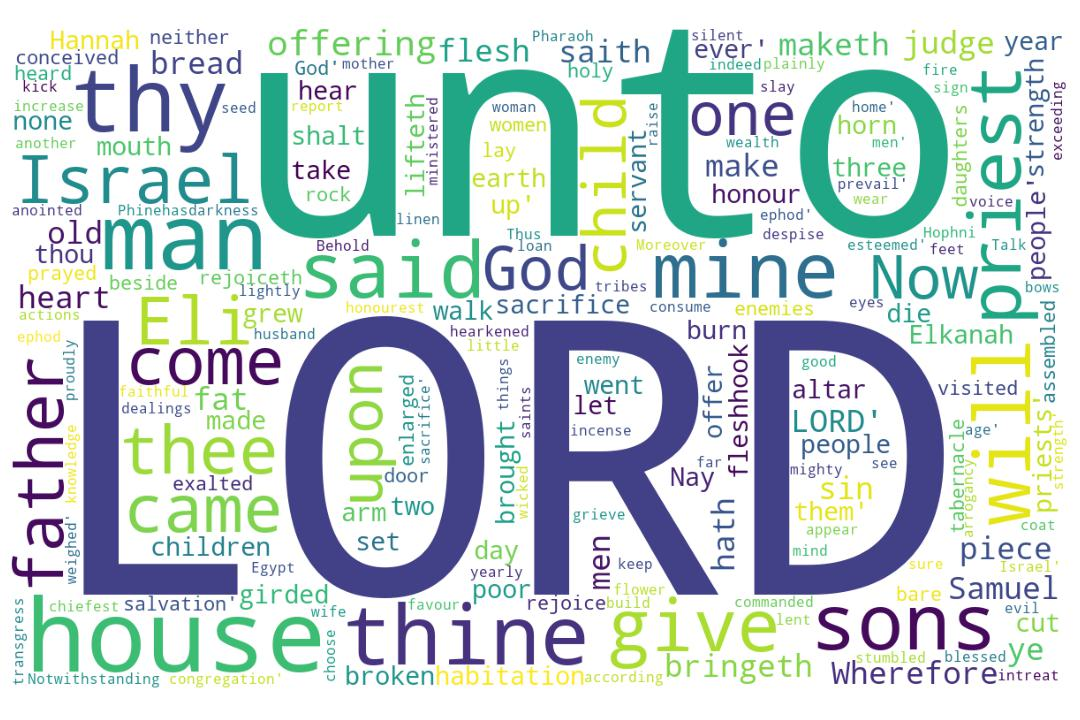
\includegraphics[width=\linewidth]{09OT-1Samuel/1Samuel2-WordCloud.jpg}
  \caption{1 Samuel 2 Word Cloud}
  \label{fig:1 Samuel 2 Word Cloud}
\end{figure}




\marginpar{\scriptsize \centering \fcolorbox{bone}{lime}{\textbf{HANNAH's HAPPINESS}}\\ (1 Samuel 2:1-11) \begin{compactenum}[I.][8]
    \item Her \textbf{Prayer}  \index[scripture]{1Samuel!1Sa 02:01}(1Sa 2:1) 
    \item Her \textbf{Proof}  \index[scripture]{1Samuel!1Sa 02:01}(1Sa 2:1)
    \item Her \textbf{Praise}  \index[scripture]{1Samuel!1Sa 02:02--02}(1Sa 2:2--3)
    \item Her \textbf{Perspective}  %\index[scripture]{1Samuel!1Sa 02:02--02}(1Sa 2:2--3)
    \item Her \textbf{Comparisons} \index[scripture]{1Samuel!1Sa 02:04--08}  (1Sa 2:4--8)
    \item Her \textbf{Prophecy}  \index[scripture]{1Samuel!1Sa 02:10}(1Sa 2:10)
    \item Her \textbf{Performance}  \index[scripture]{1Samuel!1Sa 02:11}(1Sa 2:11) -- fulfills her promise
\end{compactenum}}






\footnote{\textcolor[cmyk]{0.99998,1,0,0}{\hyperlink{TOC}{Return to end of Table of Contents.}}}\footnote{\href{https://audiobible.com/bible/1_samuel_2.html}{\textcolor[cmyk]{0.99998,1,0,0}{1 Samuel 2 Audio}}}\textcolor[cmyk]{0.99998,1,0,0}{And Hannah \fcolorbox{bone}{lime}{prayed}, and said, My heart rejoiceth in the LORD, mine horn is exalted in the LORD: my mouth is \fcolorbox{bone}{lime}{enlarged} over mine enemies; because I rejoice in thy salvation.}
[2] \textcolor[cmyk]{0.99998,1,0,0}{\emph{There} \emph{is} none holy as the LORD: for \emph{there} \emph{is} none beside thee: neither \emph{is} \emph{there} any rock like our God.}
[3] \textcolor[cmyk]{0.99998,1,0,0}{Talk no more so exceeding proudly; let \emph{not} arrogancy come out of your mouth: for the LORD \emph{is} \fcolorbox{bone}{bone}{a} God of knowledge, and by him actions are \fcolorbox{bone}{lime}{weighed}.}
[4] \textcolor[cmyk]{0.99998,1,0,0}{The bows of the mighty men \emph{are} broken, and they that stumbled are girded with strength.}
[5] \textcolor[cmyk]{0.99998,1,0,0}{\emph{They} \emph{that} \emph{were} full have hired out themselves for bread; and \emph{they} \emph{that} \emph{were} hungry ceased: so that the barren hath born seven; and she that hath many children is waxed feeble.}
[6] \textcolor[cmyk]{0.99998,1,0,0}{The LORD killeth, and maketh alive: he bringeth down to the grave, and bringeth up.}
[7] \textcolor[cmyk]{0.99998,1,0,0}{The LORD maketh poor, and maketh rich: he bringeth low, and lifteth up.}
[8] \textcolor[cmyk]{0.99998,1,0,0}{He raiseth up \fcolorbox{bone}{lime}{the poor} out of the dust, \emph{and} lifteth up the beggar from the dunghill, to set \emph{them} among princes, and to make them inherit the throne of glory: for the pillars of the earth \emph{are} the LORD'S, and he hath set the world upon them.}
[9] \textcolor[cmyk]{0.99998,1,0,0}{He will keep the feet of his saints, and the wicked shall be silent in darkness; for by strength shall no man prevail.}
[10] \textcolor[cmyk]{0.99998,1,0,0}{The adversaries of the LORD shall be broken to pieces; out of heaven shall he thunder upon them: the LORD shall judge the ends of the earth; and he shall give strength \fcolorbox{bone}{bone}{unto} his king, and \fcolorbox{bone}{lime}{exalt the horn} of his anointed.}
[11] \textcolor[cmyk]{0.99998,1,0,0}{And Elkanah went to Ramah to his house. And \fcolorbox{bone}{lime}{the child did minister} \fcolorbox{bone}{bone}{unto} the LORD before Eli the priest.}\\
\\
\P \textcolor[cmyk]{0.99998,1,0,0}{Now the sons of Eli \emph{were} sons of Belial; they knew not the LORD.}
[13] \textcolor[cmyk]{0.99998,1,0,0}{And the priests' custom with the people \emph{was,} \emph{that}, when any man offered sacrifice, the priest's servant came, while the flesh was in seething, with \fcolorbox{bone}{bone}{a} fleshhook of three teeth in his hand;}
[14] \textcolor[cmyk]{0.99998,1,0,0}{And he struck \emph{it} into the pan, or kettle, or caldron, or pot; all that the fleshhook brought up the priest took for himself. So they did in Shiloh \fcolorbox{bone}{bone}{unto} all the Israelites that came thither.}
[15] \textcolor[cmyk]{0.99998,1,0,0}{Also before they burnt the fat, the priest's servant came, and said to the man that sacrificed, Give flesh to roast for the priest; for he will not have sodden flesh of thee, but raw.}
[16] \textcolor[cmyk]{0.99998,1,0,0}{And \emph{if} any man said \fcolorbox{bone}{bone}{unto} him, Let them not fail to burn the fat presently, and \emph{then} take \emph{as} \emph{much} as thy soul desireth; then he would answer him, \emph{Nay}; but thou shalt give \emph{it} \emph{me} now: and if not, I will take \emph{it} by force.}
[17] \textcolor[cmyk]{0.99998,1,0,0}{Wherefore the sin of the young men was very great before the LORD: for men abhorred the offering of the LORD.}\\
\\
\P \textcolor[cmyk]{0.99998,1,0,0}{But Samuel ministered before the LORD, \emph{being} \fcolorbox{bone}{bone}{a} child, girded with \fcolorbox{bone}{bone}{a} linen ephod.}
[19] \textcolor[cmyk]{0.99998,1,0,0}{Moreover his mother made him \fcolorbox{bone}{bone}{a} little coat, and brought \emph{it} to him from year to year, when she came up with her husband to offer the yearly sacrifice.}\\
\\
\P \textcolor[cmyk]{0.99998,1,0,0}{And Eli blessed Elkanah and his wife, and said, The LORD give thee seed of this woman for the loan which is lent to the LORD. And they went \fcolorbox{bone}{bone}{unto} their own home.}
[21] \textcolor[cmyk]{0.99998,1,0,0}{And the LORD visited Hannah, so that she conceived, and bare three sons and two daughters. And the child Samuel grew before the LORD.}\\
\\
\P \textcolor[cmyk]{0.99998,1,0,0}{Now Eli was very old, and heard all that his sons did \fcolorbox{bone}{bone}{unto} all Israel; and how they lay with the women that assembled \emph{at} the door of the tabernacle of the congregation.}
[23] \textcolor[cmyk]{0.99998,1,0,0}{And he said \fcolorbox{bone}{bone}{unto} them, Why do ye such things? for I hear of your evil dealings by all this people.}
[24] \textcolor[cmyk]{0.99998,1,0,0}{Nay, my sons; for \emph{it} \emph{is} no good report that I hear: ye make the LORD'S people to transgress.}
[25] \textcolor[cmyk]{0.99998,1,0,0}{If one man sin against another, the judge shall judge him: but if \fcolorbox{bone}{bone}{a} man sin against the LORD, who shall intreat for him? Notwithstanding they hearkened not \fcolorbox{bone}{bone}{unto} the voice of their father, because the LORD would slay them.}
[26] \textcolor[cmyk]{0.99998,1,0,0}{And the child Samuel grew on, and was in favour both with the LORD, and also with men.}\\
\\
\P \textcolor[cmyk]{0.99998,1,0,0}{And there came \fcolorbox{bone}{bone}{a} man of God \fcolorbox{bone}{bone}{unto} Eli, and said \fcolorbox{bone}{bone}{unto} him, Thus saith the LORD, Did I plainly appear \fcolorbox{bone}{bone}{unto} the house of thy father, when they were in Egypt in Pharaoh's house?}
[28] \textcolor[cmyk]{0.99998,1,0,0}{And did I choose him out of all the tribes of Israel \emph{to} \emph{be} my priest, to offer upon mine altar, to burn incense, to wear an ephod before me? and did I give \fcolorbox{bone}{bone}{unto} the house of thy father all the offerings made by fire of the children of Israel?}
[29] \textcolor[cmyk]{0.99998,1,0,0}{Wherefore kick ye at my sacrifice and at mine offering, which I have commanded \emph{in} \emph{my} habitation; and honourest thy sons above me, to make yourselves fat with the chiefest of all the offerings of Israel my people?}
[30] \textcolor[cmyk]{0.99998,1,0,0}{Wherefore the LORD God of Israel saith, I said indeed \emph{that} thy house, and the house of thy father, should walk before me for ever: but now the LORD saith, Be it far from me; for them that honour me I will honour, and they that despise me shall be lightly esteemed.}
[31] \textcolor[cmyk]{0.99998,1,0,0}{Behold, the days come, that I will cut off thine arm, and the arm of thy father's house, that there shall not be an old man in thine house.}
[32] \textcolor[cmyk]{0.99998,1,0,0}{And thou shalt see an enemy \emph{in} \emph{my} habitation, in all \emph{the} \emph{wealth} which \emph{God} shall give Israel: and there shall not be an old man in thine house for ever.}
[33] \textcolor[cmyk]{0.99998,1,0,0}{And the man of thine, \emph{whom} I shall not cut off from mine altar, \emph{shall} \emph{be} to consume thine eyes, and to grieve thine heart: and all the increase of thine house shall die in the flower of their age.}
[34] \textcolor[cmyk]{0.99998,1,0,0}{And this \emph{shall} \emph{be} \fcolorbox{bone}{bone}{a} sign \fcolorbox{bone}{bone}{unto} thee, that shall come upon thy two sons, on Hophni and Phinehas; in one day they shall die both of them.}
[35] \textcolor[cmyk]{0.99998,1,0,0}{And I will raise me up \fcolorbox{bone}{bone}{a} faithful priest, \emph{that} shall do according to \emph{that} which \emph{is} in mine heart and in my mind: and I will build him \fcolorbox{bone}{bone}{a} sure house; and he shall walk before mine anointed for ever.}
[36] \textcolor[cmyk]{0.99998,1,0,0}{And it shall come to pass, \emph{that} every one that is left in thine house shall come \emph{and} crouch to him for \fcolorbox{bone}{bone}{a} piece of silver and \fcolorbox{bone}{bone}{a} morsel of bread, and shall say, Put me, I pray thee, into one of the priests' offices, that I may eat \fcolorbox{bone}{bone}{a} piece of bread.}
\section{1 Samuel 2 Comments}

\subsection{Numeric Nuggets}
\textbf{13: } Verse 7 has 13 words. Verses 6 and 18 have 13 unique words. The words ``a'' and ``unto'' are used 13 times in the chapter.
%\index[NWIV]{27!1Samuel!1Sa 12:1}\index[AWIP]{And!1Samuel!1Sa 12:1}\index[AWIP]{Samuel!1Samuel!1Sa 12:1}\index[AWIP]{said!1Samuel!1Sa 12:1}\index[AWIP]{said!1Samuel!1Sa 12:1 (2)}\index[AWIP]{unto!1Samuel!1Sa 12:1}\index[AWIP]{unto!1Samuel!1Sa 12:1 (2)}\index[AWIP]{unto!1Samuel!1Sa 12:1 (3)}\index[AWIP]{all!1Samuel!1Sa 12:1}\index[AWIP]{all!1Samuel!1Sa 12:1 (2)}\index[AWIP]{Israel!1Samuel!1Sa 12:1}\index[AWIP]{Behold!1Samuel!1Sa 12:1}\index[AWIP]{I!1Samuel!1Sa 12:1}\index[AWIP]{have!1Samuel!1Sa 12:1}\index[AWIP]{have!1Samuel!1Sa 12:1 (2)}\index[AWIP]{hearkened!1Samuel!1Sa 12:1}\index[AWIP]{your!1Samuel!1Sa 12:1}\index[AWIP]{voice!1Samuel!1Sa 12:1}\index[AWIP]{in!1Samuel!1Sa 12:1}\index[AWIP]{that!1Samuel!1Sa 12:1}\index[AWIP]{ye!1Samuel!1Sa 12:1}\index[AWIP]{me!1Samuel!1Sa 12:1}\index[AWIP]{and!1Samuel!1Sa 12:1}\index[AWIP]{made!1Samuel!1Sa 12:1}\index[AWIP]{a!1Samuel!1Sa 12:1}\index[AWIP]{king!1Samuel!1Sa 12:1}\index[AWIP]{over!1Samuel!1Sa 12:1}\index[AWIP]{you!1Samuel!1Sa 12:1}

\index[NWIV]{33!1Samuel!1Sa 12:2}\index[AWIP]{And!1Samuel!1Sa 12:2}\index[AWIP]{now!1Samuel!1Sa 12:2}\index[AWIP]{behold!1Samuel!1Sa 12:2}\index[AWIP]{behold!1Samuel!1Sa 12:2 (2)}\index[AWIP]{the!1Samuel!1Sa 12:2}\index[AWIP]{king!1Samuel!1Sa 12:2}\index[AWIP]{walketh!1Samuel!1Sa 12:2}\index[AWIP]{before!1Samuel!1Sa 12:2}\index[AWIP]{before!1Samuel!1Sa 12:2 (2)}\index[AWIP]{you!1Samuel!1Sa 12:2}\index[AWIP]{you!1Samuel!1Sa 12:2 (2)}\index[AWIP]{you!1Samuel!1Sa 12:2 (3)}\index[AWIP]{and!1Samuel!1Sa 12:2}\index[AWIP]{and!1Samuel!1Sa 12:2 (2)}\index[AWIP]{and!1Samuel!1Sa 12:2 (3)}\index[AWIP]{and!1Samuel!1Sa 12:2 (4)}\index[AWIP]{I!1Samuel!1Sa 12:2}\index[AWIP]{I!1Samuel!1Sa 12:2 (2)}\index[AWIP]{am!1Samuel!1Sa 12:2}\index[AWIP]{old!1Samuel!1Sa 12:2}\index[AWIP]{grayheaded!1Samuel!1Sa 12:2}\index[AWIP]{my!1Samuel!1Sa 12:2}\index[AWIP]{my!1Samuel!1Sa 12:2 (2)}\index[AWIP]{sons!1Samuel!1Sa 12:2}\index[AWIP]{\emph{are}!1Samuel!1Sa 12:2}\index[AWIP]{with!1Samuel!1Sa 12:2}\index[AWIP]{have!1Samuel!1Sa 12:2}\index[AWIP]{walked!1Samuel!1Sa 12:2}\index[AWIP]{from!1Samuel!1Sa 12:2}\index[AWIP]{childhood!1Samuel!1Sa 12:2}\index[AWIP]{unto!1Samuel!1Sa 12:2}\index[AWIP]{this!1Samuel!1Sa 12:2}\index[AWIP]{day!1Samuel!1Sa 12:2}\index[AWIP]{\emph{are}!1Samuel!1Sa 12:2}

\index[NWIV]{54!1Samuel!1Sa 12:3}\index[AWIP]{Behold!1Samuel!1Sa 12:3}\index[AWIP]{here!1Samuel!1Sa 12:3}\index[AWIP]{I!1Samuel!1Sa 12:3}\index[AWIP]{I!1Samuel!1Sa 12:3 (2)}\index[AWIP]{I!1Samuel!1Sa 12:3 (3)}\index[AWIP]{I!1Samuel!1Sa 12:3 (4)}\index[AWIP]{I!1Samuel!1Sa 12:3 (5)}\index[AWIP]{I!1Samuel!1Sa 12:3 (6)}\index[AWIP]{I!1Samuel!1Sa 12:3 (7)}\index[AWIP]{\emph{am}!1Samuel!1Sa 12:3}\index[AWIP]{witness!1Samuel!1Sa 12:3}\index[AWIP]{against!1Samuel!1Sa 12:3}\index[AWIP]{me!1Samuel!1Sa 12:3}\index[AWIP]{before!1Samuel!1Sa 12:3}\index[AWIP]{before!1Samuel!1Sa 12:3 (2)}\index[AWIP]{the!1Samuel!1Sa 12:3}\index[AWIP]{LORD!1Samuel!1Sa 12:3}\index[AWIP]{and!1Samuel!1Sa 12:3}\index[AWIP]{and!1Samuel!1Sa 12:3 (2)}\index[AWIP]{his!1Samuel!1Sa 12:3}\index[AWIP]{anointed!1Samuel!1Sa 12:3}\index[AWIP]{whose!1Samuel!1Sa 12:3}\index[AWIP]{whose!1Samuel!1Sa 12:3 (2)}\index[AWIP]{whose!1Samuel!1Sa 12:3 (3)}\index[AWIP]{ox!1Samuel!1Sa 12:3}\index[AWIP]{have!1Samuel!1Sa 12:3}\index[AWIP]{have!1Samuel!1Sa 12:3 (2)}\index[AWIP]{have!1Samuel!1Sa 12:3 (3)}\index[AWIP]{have!1Samuel!1Sa 12:3 (4)}\index[AWIP]{have!1Samuel!1Sa 12:3 (5)}\index[AWIP]{taken?!1Samuel!1Sa 12:3}\index[AWIP]{taken?!1Samuel!1Sa 12:3 (2)}\index[AWIP]{or!1Samuel!1Sa 12:3}\index[AWIP]{or!1Samuel!1Sa 12:3 (2)}\index[AWIP]{or!1Samuel!1Sa 12:3 (3)}\index[AWIP]{ass!1Samuel!1Sa 12:3}\index[AWIP]{whom!1Samuel!1Sa 12:3}\index[AWIP]{whom!1Samuel!1Sa 12:3 (2)}\index[AWIP]{defrauded?!1Samuel!1Sa 12:3}\index[AWIP]{oppressed?!1Samuel!1Sa 12:3}\index[AWIP]{of!1Samuel!1Sa 12:3}\index[AWIP]{hand!1Samuel!1Sa 12:3}\index[AWIP]{received!1Samuel!1Sa 12:3}\index[AWIP]{\emph{any}!1Samuel!1Sa 12:3}\index[AWIP]{bribe!1Samuel!1Sa 12:3}\index[AWIP]{to!1Samuel!1Sa 12:3}\index[AWIP]{blind!1Samuel!1Sa 12:3}\index[AWIP]{mine!1Samuel!1Sa 12:3}\index[AWIP]{eyes!1Samuel!1Sa 12:3}\index[AWIP]{therewith?!1Samuel!1Sa 12:3}\index[AWIP]{will!1Samuel!1Sa 12:3}\index[AWIP]{restore!1Samuel!1Sa 12:3}\index[AWIP]{it!1Samuel!1Sa 12:3}\index[AWIP]{you!1Samuel!1Sa 12:3}\index[AWIP]{\emph{am}!1Samuel!1Sa 12:3}\index[AWIP]{\emph{any}!1Samuel!1Sa 12:3}

\index[NWIV]{20!1Samuel!1Sa 12:4}\index[AWIP]{And!1Samuel!1Sa 12:4}\index[AWIP]{they!1Samuel!1Sa 12:4}\index[AWIP]{said!1Samuel!1Sa 12:4}\index[AWIP]{Thou!1Samuel!1Sa 12:4}\index[AWIP]{hast!1Samuel!1Sa 12:4}\index[AWIP]{hast!1Samuel!1Sa 12:4 (2)}\index[AWIP]{not!1Samuel!1Sa 12:4}\index[AWIP]{defrauded!1Samuel!1Sa 12:4}\index[AWIP]{us!1Samuel!1Sa 12:4}\index[AWIP]{us!1Samuel!1Sa 12:4 (2)}\index[AWIP]{nor!1Samuel!1Sa 12:4}\index[AWIP]{oppressed!1Samuel!1Sa 12:4}\index[AWIP]{neither!1Samuel!1Sa 12:4}\index[AWIP]{thou!1Samuel!1Sa 12:4}\index[AWIP]{taken!1Samuel!1Sa 12:4}\index[AWIP]{ought!1Samuel!1Sa 12:4}\index[AWIP]{of!1Samuel!1Sa 12:4}\index[AWIP]{any!1Samuel!1Sa 12:4}\index[AWIP]{man's!1Samuel!1Sa 12:4}\index[AWIP]{hand!1Samuel!1Sa 12:4}

\index[NWIV]{33!1Samuel!1Sa 12:5}\index[AWIP]{And!1Samuel!1Sa 12:5}\index[AWIP]{And!1Samuel!1Sa 12:5 (2)}\index[AWIP]{he!1Samuel!1Sa 12:5}\index[AWIP]{said!1Samuel!1Sa 12:5}\index[AWIP]{unto!1Samuel!1Sa 12:5}\index[AWIP]{them!1Samuel!1Sa 12:5}\index[AWIP]{The!1Samuel!1Sa 12:5}\index[AWIP]{LORD!1Samuel!1Sa 12:5}\index[AWIP]{\emph{is}!1Samuel!1Sa 12:5}\index[AWIP]{\emph{is}!1Samuel!1Sa 12:5 (2)}\index[AWIP]{\emph{is}!1Samuel!1Sa 12:5 (3)}\index[AWIP]{witness!1Samuel!1Sa 12:5}\index[AWIP]{witness!1Samuel!1Sa 12:5 (2)}\index[AWIP]{witness!1Samuel!1Sa 12:5 (3)}\index[AWIP]{against!1Samuel!1Sa 12:5}\index[AWIP]{you!1Samuel!1Sa 12:5}\index[AWIP]{and!1Samuel!1Sa 12:5}\index[AWIP]{his!1Samuel!1Sa 12:5}\index[AWIP]{anointed!1Samuel!1Sa 12:5}\index[AWIP]{this!1Samuel!1Sa 12:5}\index[AWIP]{day!1Samuel!1Sa 12:5}\index[AWIP]{that!1Samuel!1Sa 12:5}\index[AWIP]{ye!1Samuel!1Sa 12:5}\index[AWIP]{have!1Samuel!1Sa 12:5}\index[AWIP]{not!1Samuel!1Sa 12:5}\index[AWIP]{found!1Samuel!1Sa 12:5}\index[AWIP]{ought!1Samuel!1Sa 12:5}\index[AWIP]{in!1Samuel!1Sa 12:5}\index[AWIP]{my!1Samuel!1Sa 12:5}\index[AWIP]{hand!1Samuel!1Sa 12:5}\index[AWIP]{they!1Samuel!1Sa 12:5}\index[AWIP]{answered!1Samuel!1Sa 12:5}\index[AWIP]{\emph{He}!1Samuel!1Sa 12:5}\index[AWIP]{\emph{is}!1Samuel!1Sa 12:5}\index[AWIP]{\emph{is}!1Samuel!1Sa 12:5 (2)}\index[AWIP]{\emph{is}!1Samuel!1Sa 12:5 (3)}\index[AWIP]{\emph{He}!1Samuel!1Sa 12:5}

\index[NWIV]{27!1Samuel!1Sa 12:6}\index[AWIP]{And!1Samuel!1Sa 12:6}\index[AWIP]{Samuel!1Samuel!1Sa 12:6}\index[AWIP]{said!1Samuel!1Sa 12:6}\index[AWIP]{unto!1Samuel!1Sa 12:6}\index[AWIP]{the!1Samuel!1Sa 12:6}\index[AWIP]{the!1Samuel!1Sa 12:6 (2)}\index[AWIP]{the!1Samuel!1Sa 12:6 (3)}\index[AWIP]{people!1Samuel!1Sa 12:6}\index[AWIP]{\emph{It}!1Samuel!1Sa 12:6}\index[AWIP]{\emph{is}!1Samuel!1Sa 12:6}\index[AWIP]{LORD!1Samuel!1Sa 12:6}\index[AWIP]{that!1Samuel!1Sa 12:6}\index[AWIP]{that!1Samuel!1Sa 12:6 (2)}\index[AWIP]{advanced!1Samuel!1Sa 12:6}\index[AWIP]{Moses!1Samuel!1Sa 12:6}\index[AWIP]{and!1Samuel!1Sa 12:6}\index[AWIP]{and!1Samuel!1Sa 12:6 (2)}\index[AWIP]{Aaron!1Samuel!1Sa 12:6}\index[AWIP]{brought!1Samuel!1Sa 12:6}\index[AWIP]{your!1Samuel!1Sa 12:6}\index[AWIP]{fathers!1Samuel!1Sa 12:6}\index[AWIP]{up!1Samuel!1Sa 12:6}\index[AWIP]{out!1Samuel!1Sa 12:6}\index[AWIP]{of!1Samuel!1Sa 12:6}\index[AWIP]{of!1Samuel!1Sa 12:6 (2)}\index[AWIP]{land!1Samuel!1Sa 12:6}\index[AWIP]{Egypt!1Samuel!1Sa 12:6}\index[AWIP]{\emph{It}!1Samuel!1Sa 12:6}\index[AWIP]{\emph{is}!1Samuel!1Sa 12:6}

\index[NWIV]{30!1Samuel!1Sa 12:7}\index[AWIP]{Now!1Samuel!1Sa 12:7}\index[AWIP]{therefore!1Samuel!1Sa 12:7}\index[AWIP]{stand!1Samuel!1Sa 12:7}\index[AWIP]{still!1Samuel!1Sa 12:7}\index[AWIP]{that!1Samuel!1Sa 12:7}\index[AWIP]{I!1Samuel!1Sa 12:7}\index[AWIP]{may!1Samuel!1Sa 12:7}\index[AWIP]{reason!1Samuel!1Sa 12:7}\index[AWIP]{with!1Samuel!1Sa 12:7}\index[AWIP]{you!1Samuel!1Sa 12:7}\index[AWIP]{you!1Samuel!1Sa 12:7 (2)}\index[AWIP]{before!1Samuel!1Sa 12:7}\index[AWIP]{the!1Samuel!1Sa 12:7}\index[AWIP]{the!1Samuel!1Sa 12:7 (2)}\index[AWIP]{the!1Samuel!1Sa 12:7 (3)}\index[AWIP]{LORD!1Samuel!1Sa 12:7}\index[AWIP]{LORD!1Samuel!1Sa 12:7 (2)}\index[AWIP]{of!1Samuel!1Sa 12:7}\index[AWIP]{of!1Samuel!1Sa 12:7 (2)}\index[AWIP]{all!1Samuel!1Sa 12:7}\index[AWIP]{righteous!1Samuel!1Sa 12:7}\index[AWIP]{acts!1Samuel!1Sa 12:7}\index[AWIP]{which!1Samuel!1Sa 12:7}\index[AWIP]{he!1Samuel!1Sa 12:7}\index[AWIP]{did!1Samuel!1Sa 12:7}\index[AWIP]{to!1Samuel!1Sa 12:7}\index[AWIP]{to!1Samuel!1Sa 12:7 (2)}\index[AWIP]{and!1Samuel!1Sa 12:7}\index[AWIP]{your!1Samuel!1Sa 12:7}\index[AWIP]{fathers!1Samuel!1Sa 12:7}

\index[NWIV]{35!1Samuel!1Sa 12:8}\index[AWIP]{When!1Samuel!1Sa 12:8}\index[AWIP]{Jacob!1Samuel!1Sa 12:8}\index[AWIP]{was!1Samuel!1Sa 12:8}\index[AWIP]{come!1Samuel!1Sa 12:8}\index[AWIP]{into!1Samuel!1Sa 12:8}\index[AWIP]{Egypt!1Samuel!1Sa 12:8}\index[AWIP]{Egypt!1Samuel!1Sa 12:8 (2)}\index[AWIP]{and!1Samuel!1Sa 12:8}\index[AWIP]{and!1Samuel!1Sa 12:8 (2)}\index[AWIP]{and!1Samuel!1Sa 12:8 (3)}\index[AWIP]{your!1Samuel!1Sa 12:8}\index[AWIP]{your!1Samuel!1Sa 12:8 (2)}\index[AWIP]{fathers!1Samuel!1Sa 12:8}\index[AWIP]{fathers!1Samuel!1Sa 12:8 (2)}\index[AWIP]{cried!1Samuel!1Sa 12:8}\index[AWIP]{unto!1Samuel!1Sa 12:8}\index[AWIP]{the!1Samuel!1Sa 12:8}\index[AWIP]{the!1Samuel!1Sa 12:8 (2)}\index[AWIP]{LORD!1Samuel!1Sa 12:8}\index[AWIP]{LORD!1Samuel!1Sa 12:8 (2)}\index[AWIP]{then!1Samuel!1Sa 12:8}\index[AWIP]{sent!1Samuel!1Sa 12:8}\index[AWIP]{Moses!1Samuel!1Sa 12:8}\index[AWIP]{Aaron!1Samuel!1Sa 12:8}\index[AWIP]{which!1Samuel!1Sa 12:8}\index[AWIP]{brought!1Samuel!1Sa 12:8}\index[AWIP]{forth!1Samuel!1Sa 12:8}\index[AWIP]{out!1Samuel!1Sa 12:8}\index[AWIP]{of!1Samuel!1Sa 12:8}\index[AWIP]{made!1Samuel!1Sa 12:8}\index[AWIP]{them!1Samuel!1Sa 12:8}\index[AWIP]{dwell!1Samuel!1Sa 12:8}\index[AWIP]{in!1Samuel!1Sa 12:8}\index[AWIP]{this!1Samuel!1Sa 12:8}\index[AWIP]{place!1Samuel!1Sa 12:8}

\index[NWIV]{43!1Samuel!1Sa 12:9}\index[AWIP]{And!1Samuel!1Sa 12:9}\index[AWIP]{when!1Samuel!1Sa 12:9}\index[AWIP]{they!1Samuel!1Sa 12:9}\index[AWIP]{they!1Samuel!1Sa 12:9 (2)}\index[AWIP]{forgat!1Samuel!1Sa 12:9}\index[AWIP]{the!1Samuel!1Sa 12:9}\index[AWIP]{the!1Samuel!1Sa 12:9 (2)}\index[AWIP]{the!1Samuel!1Sa 12:9 (3)}\index[AWIP]{the!1Samuel!1Sa 12:9 (4)}\index[AWIP]{the!1Samuel!1Sa 12:9 (5)}\index[AWIP]{the!1Samuel!1Sa 12:9 (6)}\index[AWIP]{the!1Samuel!1Sa 12:9 (7)}\index[AWIP]{LORD!1Samuel!1Sa 12:9}\index[AWIP]{their!1Samuel!1Sa 12:9}\index[AWIP]{God!1Samuel!1Sa 12:9}\index[AWIP]{he!1Samuel!1Sa 12:9}\index[AWIP]{sold!1Samuel!1Sa 12:9}\index[AWIP]{them!1Samuel!1Sa 12:9}\index[AWIP]{them!1Samuel!1Sa 12:9 (2)}\index[AWIP]{into!1Samuel!1Sa 12:9}\index[AWIP]{into!1Samuel!1Sa 12:9 (2)}\index[AWIP]{into!1Samuel!1Sa 12:9 (3)}\index[AWIP]{hand!1Samuel!1Sa 12:9}\index[AWIP]{hand!1Samuel!1Sa 12:9 (2)}\index[AWIP]{hand!1Samuel!1Sa 12:9 (3)}\index[AWIP]{of!1Samuel!1Sa 12:9}\index[AWIP]{of!1Samuel!1Sa 12:9 (2)}\index[AWIP]{of!1Samuel!1Sa 12:9 (3)}\index[AWIP]{of!1Samuel!1Sa 12:9 (4)}\index[AWIP]{of!1Samuel!1Sa 12:9 (5)}\index[AWIP]{of!1Samuel!1Sa 12:9 (6)}\index[AWIP]{Sisera!1Samuel!1Sa 12:9}\index[AWIP]{captain!1Samuel!1Sa 12:9}\index[AWIP]{host!1Samuel!1Sa 12:9}\index[AWIP]{Hazor!1Samuel!1Sa 12:9}\index[AWIP]{and!1Samuel!1Sa 12:9}\index[AWIP]{and!1Samuel!1Sa 12:9 (2)}\index[AWIP]{and!1Samuel!1Sa 12:9 (3)}\index[AWIP]{Philistines!1Samuel!1Sa 12:9}\index[AWIP]{king!1Samuel!1Sa 12:9}\index[AWIP]{Moab!1Samuel!1Sa 12:9}\index[AWIP]{fought!1Samuel!1Sa 12:9}\index[AWIP]{against!1Samuel!1Sa 12:9}

\index[NWIV]{39!1Samuel!1Sa 12:10}\index[AWIP]{And!1Samuel!1Sa 12:10}\index[AWIP]{they!1Samuel!1Sa 12:10}\index[AWIP]{cried!1Samuel!1Sa 12:10}\index[AWIP]{unto!1Samuel!1Sa 12:10}\index[AWIP]{the!1Samuel!1Sa 12:10}\index[AWIP]{the!1Samuel!1Sa 12:10 (2)}\index[AWIP]{the!1Samuel!1Sa 12:10 (3)}\index[AWIP]{LORD!1Samuel!1Sa 12:10}\index[AWIP]{LORD!1Samuel!1Sa 12:10 (2)}\index[AWIP]{and!1Samuel!1Sa 12:10}\index[AWIP]{and!1Samuel!1Sa 12:10 (2)}\index[AWIP]{and!1Samuel!1Sa 12:10 (3)}\index[AWIP]{and!1Samuel!1Sa 12:10 (4)}\index[AWIP]{said!1Samuel!1Sa 12:10}\index[AWIP]{We!1Samuel!1Sa 12:10}\index[AWIP]{have!1Samuel!1Sa 12:10}\index[AWIP]{have!1Samuel!1Sa 12:10 (2)}\index[AWIP]{have!1Samuel!1Sa 12:10 (3)}\index[AWIP]{sinned!1Samuel!1Sa 12:10}\index[AWIP]{because!1Samuel!1Sa 12:10}\index[AWIP]{we!1Samuel!1Sa 12:10}\index[AWIP]{we!1Samuel!1Sa 12:10 (2)}\index[AWIP]{forsaken!1Samuel!1Sa 12:10}\index[AWIP]{served!1Samuel!1Sa 12:10}\index[AWIP]{Baalim!1Samuel!1Sa 12:10}\index[AWIP]{Ashtaroth!1Samuel!1Sa 12:10}\index[AWIP]{but!1Samuel!1Sa 12:10}\index[AWIP]{now!1Samuel!1Sa 12:10}\index[AWIP]{deliver!1Samuel!1Sa 12:10}\index[AWIP]{us!1Samuel!1Sa 12:10}\index[AWIP]{out!1Samuel!1Sa 12:10}\index[AWIP]{of!1Samuel!1Sa 12:10}\index[AWIP]{of!1Samuel!1Sa 12:10 (2)}\index[AWIP]{hand!1Samuel!1Sa 12:10}\index[AWIP]{our!1Samuel!1Sa 12:10}\index[AWIP]{enemies!1Samuel!1Sa 12:10}\index[AWIP]{will!1Samuel!1Sa 12:10}\index[AWIP]{serve!1Samuel!1Sa 12:10}\index[AWIP]{thee!1Samuel!1Sa 12:10}

\index[NWIV]{28!1Samuel!1Sa 12:11}\index[AWIP]{And!1Samuel!1Sa 12:11}\index[AWIP]{the!1Samuel!1Sa 12:11}\index[AWIP]{the!1Samuel!1Sa 12:11 (2)}\index[AWIP]{LORD!1Samuel!1Sa 12:11}\index[AWIP]{sent!1Samuel!1Sa 12:11}\index[AWIP]{Jerubbaal!1Samuel!1Sa 12:11}\index[AWIP]{and!1Samuel!1Sa 12:11}\index[AWIP]{and!1Samuel!1Sa 12:11 (2)}\index[AWIP]{and!1Samuel!1Sa 12:11 (3)}\index[AWIP]{and!1Samuel!1Sa 12:11 (4)}\index[AWIP]{and!1Samuel!1Sa 12:11 (5)}\index[AWIP]{Bedan!1Samuel!1Sa 12:11}\index[AWIP]{Jephthah!1Samuel!1Sa 12:11}\index[AWIP]{Samuel!1Samuel!1Sa 12:11}\index[AWIP]{delivered!1Samuel!1Sa 12:11}\index[AWIP]{you!1Samuel!1Sa 12:11}\index[AWIP]{out!1Samuel!1Sa 12:11}\index[AWIP]{of!1Samuel!1Sa 12:11}\index[AWIP]{of!1Samuel!1Sa 12:11 (2)}\index[AWIP]{hand!1Samuel!1Sa 12:11}\index[AWIP]{your!1Samuel!1Sa 12:11}\index[AWIP]{enemies!1Samuel!1Sa 12:11}\index[AWIP]{on!1Samuel!1Sa 12:11}\index[AWIP]{every!1Samuel!1Sa 12:11}\index[AWIP]{side!1Samuel!1Sa 12:11}\index[AWIP]{ye!1Samuel!1Sa 12:11}\index[AWIP]{dwelled!1Samuel!1Sa 12:11}\index[AWIP]{safe!1Samuel!1Sa 12:11}

\index[NWIV]{36!1Samuel!1Sa 12:12}\index[AWIP]{And!1Samuel!1Sa 12:12}\index[AWIP]{when!1Samuel!1Sa 12:12}\index[AWIP]{when!1Samuel!1Sa 12:12 (2)}\index[AWIP]{ye!1Samuel!1Sa 12:12}\index[AWIP]{ye!1Samuel!1Sa 12:12 (2)}\index[AWIP]{saw!1Samuel!1Sa 12:12}\index[AWIP]{that!1Samuel!1Sa 12:12}\index[AWIP]{Nahash!1Samuel!1Sa 12:12}\index[AWIP]{the!1Samuel!1Sa 12:12}\index[AWIP]{the!1Samuel!1Sa 12:12 (2)}\index[AWIP]{the!1Samuel!1Sa 12:12 (3)}\index[AWIP]{king!1Samuel!1Sa 12:12}\index[AWIP]{king!1Samuel!1Sa 12:12 (2)}\index[AWIP]{king!1Samuel!1Sa 12:12 (3)}\index[AWIP]{of!1Samuel!1Sa 12:12}\index[AWIP]{of!1Samuel!1Sa 12:12 (2)}\index[AWIP]{children!1Samuel!1Sa 12:12}\index[AWIP]{Ammon!1Samuel!1Sa 12:12}\index[AWIP]{came!1Samuel!1Sa 12:12}\index[AWIP]{against!1Samuel!1Sa 12:12}\index[AWIP]{you!1Samuel!1Sa 12:12}\index[AWIP]{said!1Samuel!1Sa 12:12}\index[AWIP]{unto!1Samuel!1Sa 12:12}\index[AWIP]{me!1Samuel!1Sa 12:12}\index[AWIP]{Nay!1Samuel!1Sa 12:12}\index[AWIP]{but!1Samuel!1Sa 12:12}\index[AWIP]{a!1Samuel!1Sa 12:12}\index[AWIP]{shall!1Samuel!1Sa 12:12}\index[AWIP]{reign!1Samuel!1Sa 12:12}\index[AWIP]{over!1Samuel!1Sa 12:12}\index[AWIP]{us!1Samuel!1Sa 12:12}\index[AWIP]{LORD!1Samuel!1Sa 12:12}\index[AWIP]{your!1Samuel!1Sa 12:12}\index[AWIP]{your!1Samuel!1Sa 12:12 (2)}\index[AWIP]{God!1Samuel!1Sa 12:12}\index[AWIP]{\emph{was}!1Samuel!1Sa 12:12}\index[AWIP]{\emph{was}!1Samuel!1Sa 12:12}

\index[NWIV]{24!1Samuel!1Sa 12:13}\index[AWIP]{Now!1Samuel!1Sa 12:13}\index[AWIP]{therefore!1Samuel!1Sa 12:13}\index[AWIP]{behold!1Samuel!1Sa 12:13}\index[AWIP]{behold!1Samuel!1Sa 12:13 (2)}\index[AWIP]{the!1Samuel!1Sa 12:13}\index[AWIP]{the!1Samuel!1Sa 12:13 (2)}\index[AWIP]{king!1Samuel!1Sa 12:13}\index[AWIP]{king!1Samuel!1Sa 12:13 (2)}\index[AWIP]{whom!1Samuel!1Sa 12:13}\index[AWIP]{whom!1Samuel!1Sa 12:13 (2)}\index[AWIP]{ye!1Samuel!1Sa 12:13}\index[AWIP]{ye!1Samuel!1Sa 12:13 (2)}\index[AWIP]{have!1Samuel!1Sa 12:13}\index[AWIP]{have!1Samuel!1Sa 12:13 (2)}\index[AWIP]{chosen!1Samuel!1Sa 12:13}\index[AWIP]{\emph{and}!1Samuel!1Sa 12:13}\index[AWIP]{desired!!1Samuel!1Sa 12:13}\index[AWIP]{and!1Samuel!1Sa 12:13}\index[AWIP]{LORD!1Samuel!1Sa 12:13}\index[AWIP]{hath!1Samuel!1Sa 12:13}\index[AWIP]{set!1Samuel!1Sa 12:13}\index[AWIP]{a!1Samuel!1Sa 12:13}\index[AWIP]{over!1Samuel!1Sa 12:13}\index[AWIP]{you!1Samuel!1Sa 12:13}\index[AWIP]{\emph{and}!1Samuel!1Sa 12:13}

\index[NWIV]{40!1Samuel!1Sa 12:14}\index[AWIP]{If!1Samuel!1Sa 12:14}\index[AWIP]{ye!1Samuel!1Sa 12:14}\index[AWIP]{ye!1Samuel!1Sa 12:14 (2)}\index[AWIP]{will!1Samuel!1Sa 12:14}\index[AWIP]{fear!1Samuel!1Sa 12:14}\index[AWIP]{the!1Samuel!1Sa 12:14}\index[AWIP]{the!1Samuel!1Sa 12:14 (2)}\index[AWIP]{the!1Samuel!1Sa 12:14 (3)}\index[AWIP]{the!1Samuel!1Sa 12:14 (4)}\index[AWIP]{the!1Samuel!1Sa 12:14 (5)}\index[AWIP]{LORD!1Samuel!1Sa 12:14}\index[AWIP]{LORD!1Samuel!1Sa 12:14 (2)}\index[AWIP]{LORD!1Samuel!1Sa 12:14 (3)}\index[AWIP]{and!1Samuel!1Sa 12:14}\index[AWIP]{and!1Samuel!1Sa 12:14 (2)}\index[AWIP]{and!1Samuel!1Sa 12:14 (3)}\index[AWIP]{and!1Samuel!1Sa 12:14 (4)}\index[AWIP]{serve!1Samuel!1Sa 12:14}\index[AWIP]{him!1Samuel!1Sa 12:14}\index[AWIP]{obey!1Samuel!1Sa 12:14}\index[AWIP]{his!1Samuel!1Sa 12:14}\index[AWIP]{voice!1Samuel!1Sa 12:14}\index[AWIP]{not!1Samuel!1Sa 12:14}\index[AWIP]{rebel!1Samuel!1Sa 12:14}\index[AWIP]{against!1Samuel!1Sa 12:14}\index[AWIP]{commandment!1Samuel!1Sa 12:14}\index[AWIP]{of!1Samuel!1Sa 12:14}\index[AWIP]{then!1Samuel!1Sa 12:14}\index[AWIP]{shall!1Samuel!1Sa 12:14}\index[AWIP]{both!1Samuel!1Sa 12:14}\index[AWIP]{also!1Samuel!1Sa 12:14}\index[AWIP]{king!1Samuel!1Sa 12:14}\index[AWIP]{that!1Samuel!1Sa 12:14}\index[AWIP]{reigneth!1Samuel!1Sa 12:14}\index[AWIP]{over!1Samuel!1Sa 12:14}\index[AWIP]{you!1Samuel!1Sa 12:14}\index[AWIP]{continue!1Samuel!1Sa 12:14}\index[AWIP]{following!1Samuel!1Sa 12:14}\index[AWIP]{your!1Samuel!1Sa 12:14}\index[AWIP]{God!1Samuel!1Sa 12:14}

\index[NWIV]{35!1Samuel!1Sa 12:15}\index[AWIP]{But!1Samuel!1Sa 12:15}\index[AWIP]{if!1Samuel!1Sa 12:15}\index[AWIP]{ye!1Samuel!1Sa 12:15}\index[AWIP]{will!1Samuel!1Sa 12:15}\index[AWIP]{not!1Samuel!1Sa 12:15}\index[AWIP]{obey!1Samuel!1Sa 12:15}\index[AWIP]{the!1Samuel!1Sa 12:15}\index[AWIP]{the!1Samuel!1Sa 12:15 (2)}\index[AWIP]{the!1Samuel!1Sa 12:15 (3)}\index[AWIP]{the!1Samuel!1Sa 12:15 (4)}\index[AWIP]{the!1Samuel!1Sa 12:15 (5)}\index[AWIP]{the!1Samuel!1Sa 12:15 (6)}\index[AWIP]{voice!1Samuel!1Sa 12:15}\index[AWIP]{of!1Samuel!1Sa 12:15}\index[AWIP]{of!1Samuel!1Sa 12:15 (2)}\index[AWIP]{of!1Samuel!1Sa 12:15 (3)}\index[AWIP]{LORD!1Samuel!1Sa 12:15}\index[AWIP]{LORD!1Samuel!1Sa 12:15 (2)}\index[AWIP]{LORD!1Samuel!1Sa 12:15 (3)}\index[AWIP]{but!1Samuel!1Sa 12:15}\index[AWIP]{rebel!1Samuel!1Sa 12:15}\index[AWIP]{against!1Samuel!1Sa 12:15}\index[AWIP]{against!1Samuel!1Sa 12:15 (2)}\index[AWIP]{against!1Samuel!1Sa 12:15 (3)}\index[AWIP]{commandment!1Samuel!1Sa 12:15}\index[AWIP]{then!1Samuel!1Sa 12:15}\index[AWIP]{shall!1Samuel!1Sa 12:15}\index[AWIP]{hand!1Samuel!1Sa 12:15}\index[AWIP]{be!1Samuel!1Sa 12:15}\index[AWIP]{you!1Samuel!1Sa 12:15}\index[AWIP]{as!1Samuel!1Sa 12:15}\index[AWIP]{\emph{it}!1Samuel!1Sa 12:15}\index[AWIP]{\emph{was}!1Samuel!1Sa 12:15}\index[AWIP]{your!1Samuel!1Sa 12:15}\index[AWIP]{fathers!1Samuel!1Sa 12:15}\index[AWIP]{\emph{it}!1Samuel!1Sa 12:15}\index[AWIP]{\emph{was}!1Samuel!1Sa 12:15}

\index[NWIV]{16!1Samuel!1Sa 12:16}\index[AWIP]{Now!1Samuel!1Sa 12:16}\index[AWIP]{therefore!1Samuel!1Sa 12:16}\index[AWIP]{stand!1Samuel!1Sa 12:16}\index[AWIP]{and!1Samuel!1Sa 12:16}\index[AWIP]{see!1Samuel!1Sa 12:16}\index[AWIP]{this!1Samuel!1Sa 12:16}\index[AWIP]{great!1Samuel!1Sa 12:16}\index[AWIP]{thing!1Samuel!1Sa 12:16}\index[AWIP]{which!1Samuel!1Sa 12:16}\index[AWIP]{the!1Samuel!1Sa 12:16}\index[AWIP]{LORD!1Samuel!1Sa 12:16}\index[AWIP]{will!1Samuel!1Sa 12:16}\index[AWIP]{do!1Samuel!1Sa 12:16}\index[AWIP]{before!1Samuel!1Sa 12:16}\index[AWIP]{your!1Samuel!1Sa 12:16}\index[AWIP]{eyes!1Samuel!1Sa 12:16}

\index[NWIV]{46!1Samuel!1Sa 12:17}\index[AWIP]{\emph{Is}!1Samuel!1Sa 12:17}\index[AWIP]{\emph{it}!1Samuel!1Sa 12:17}\index[AWIP]{not!1Samuel!1Sa 12:17}\index[AWIP]{wheat!1Samuel!1Sa 12:17}\index[AWIP]{harvest!1Samuel!1Sa 12:17}\index[AWIP]{to!1Samuel!1Sa 12:17}\index[AWIP]{day?!1Samuel!1Sa 12:17}\index[AWIP]{I!1Samuel!1Sa 12:17}\index[AWIP]{will!1Samuel!1Sa 12:17}\index[AWIP]{call!1Samuel!1Sa 12:17}\index[AWIP]{unto!1Samuel!1Sa 12:17}\index[AWIP]{the!1Samuel!1Sa 12:17}\index[AWIP]{the!1Samuel!1Sa 12:17 (2)}\index[AWIP]{the!1Samuel!1Sa 12:17 (3)}\index[AWIP]{LORD!1Samuel!1Sa 12:17}\index[AWIP]{LORD!1Samuel!1Sa 12:17 (2)}\index[AWIP]{and!1Samuel!1Sa 12:17}\index[AWIP]{and!1Samuel!1Sa 12:17 (2)}\index[AWIP]{and!1Samuel!1Sa 12:17 (3)}\index[AWIP]{he!1Samuel!1Sa 12:17}\index[AWIP]{shall!1Samuel!1Sa 12:17}\index[AWIP]{send!1Samuel!1Sa 12:17}\index[AWIP]{thunder!1Samuel!1Sa 12:17}\index[AWIP]{rain!1Samuel!1Sa 12:17}\index[AWIP]{that!1Samuel!1Sa 12:17}\index[AWIP]{that!1Samuel!1Sa 12:17 (2)}\index[AWIP]{ye!1Samuel!1Sa 12:17}\index[AWIP]{ye!1Samuel!1Sa 12:17 (2)}\index[AWIP]{may!1Samuel!1Sa 12:17}\index[AWIP]{perceive!1Samuel!1Sa 12:17}\index[AWIP]{see!1Samuel!1Sa 12:17}\index[AWIP]{your!1Samuel!1Sa 12:17}\index[AWIP]{wickedness!1Samuel!1Sa 12:17}\index[AWIP]{\emph{is}!1Samuel!1Sa 12:17}\index[AWIP]{great!1Samuel!1Sa 12:17}\index[AWIP]{which!1Samuel!1Sa 12:17}\index[AWIP]{have!1Samuel!1Sa 12:17}\index[AWIP]{done!1Samuel!1Sa 12:17}\index[AWIP]{in!1Samuel!1Sa 12:17}\index[AWIP]{in!1Samuel!1Sa 12:17 (2)}\index[AWIP]{sight!1Samuel!1Sa 12:17}\index[AWIP]{of!1Samuel!1Sa 12:17}\index[AWIP]{asking!1Samuel!1Sa 12:17}\index[AWIP]{you!1Samuel!1Sa 12:17}\index[AWIP]{a!1Samuel!1Sa 12:17}\index[AWIP]{king!1Samuel!1Sa 12:17}\index[AWIP]{\emph{Is}!1Samuel!1Sa 12:17}\index[AWIP]{\emph{it}!1Samuel!1Sa 12:17}\index[AWIP]{\emph{is}!1Samuel!1Sa 12:17}

\index[NWIV]{25!1Samuel!1Sa 12:18}\index[AWIP]{So!1Samuel!1Sa 12:18}\index[AWIP]{Samuel!1Samuel!1Sa 12:18}\index[AWIP]{Samuel!1Samuel!1Sa 12:18 (2)}\index[AWIP]{called!1Samuel!1Sa 12:18}\index[AWIP]{unto!1Samuel!1Sa 12:18}\index[AWIP]{the!1Samuel!1Sa 12:18}\index[AWIP]{the!1Samuel!1Sa 12:18 (2)}\index[AWIP]{the!1Samuel!1Sa 12:18 (3)}\index[AWIP]{the!1Samuel!1Sa 12:18 (4)}\index[AWIP]{LORD!1Samuel!1Sa 12:18}\index[AWIP]{LORD!1Samuel!1Sa 12:18 (2)}\index[AWIP]{LORD!1Samuel!1Sa 12:18 (3)}\index[AWIP]{and!1Samuel!1Sa 12:18}\index[AWIP]{and!1Samuel!1Sa 12:18 (2)}\index[AWIP]{and!1Samuel!1Sa 12:18 (3)}\index[AWIP]{and!1Samuel!1Sa 12:18 (4)}\index[AWIP]{sent!1Samuel!1Sa 12:18}\index[AWIP]{thunder!1Samuel!1Sa 12:18}\index[AWIP]{rain!1Samuel!1Sa 12:18}\index[AWIP]{that!1Samuel!1Sa 12:18}\index[AWIP]{day!1Samuel!1Sa 12:18}\index[AWIP]{all!1Samuel!1Sa 12:18}\index[AWIP]{people!1Samuel!1Sa 12:18}\index[AWIP]{greatly!1Samuel!1Sa 12:18}\index[AWIP]{feared!1Samuel!1Sa 12:18}

\index[NWIV]{35!1Samuel!1Sa 12:19}\index[AWIP]{And!1Samuel!1Sa 12:19}\index[AWIP]{all!1Samuel!1Sa 12:19}\index[AWIP]{all!1Samuel!1Sa 12:19 (2)}\index[AWIP]{the!1Samuel!1Sa 12:19}\index[AWIP]{the!1Samuel!1Sa 12:19 (2)}\index[AWIP]{people!1Samuel!1Sa 12:19}\index[AWIP]{said!1Samuel!1Sa 12:19}\index[AWIP]{unto!1Samuel!1Sa 12:19}\index[AWIP]{unto!1Samuel!1Sa 12:19 (2)}\index[AWIP]{unto!1Samuel!1Sa 12:19 (3)}\index[AWIP]{Samuel!1Samuel!1Sa 12:19}\index[AWIP]{Pray!1Samuel!1Sa 12:19}\index[AWIP]{for!1Samuel!1Sa 12:19}\index[AWIP]{for!1Samuel!1Sa 12:19 (2)}\index[AWIP]{thy!1Samuel!1Sa 12:19}\index[AWIP]{thy!1Samuel!1Sa 12:19 (2)}\index[AWIP]{servants!1Samuel!1Sa 12:19}\index[AWIP]{LORD!1Samuel!1Sa 12:19}\index[AWIP]{God!1Samuel!1Sa 12:19}\index[AWIP]{that!1Samuel!1Sa 12:19}\index[AWIP]{we!1Samuel!1Sa 12:19}\index[AWIP]{we!1Samuel!1Sa 12:19 (2)}\index[AWIP]{die!1Samuel!1Sa 12:19}\index[AWIP]{not!1Samuel!1Sa 12:19}\index[AWIP]{have!1Samuel!1Sa 12:19}\index[AWIP]{added!1Samuel!1Sa 12:19}\index[AWIP]{our!1Samuel!1Sa 12:19}\index[AWIP]{sins!1Samuel!1Sa 12:19}\index[AWIP]{\emph{this}!1Samuel!1Sa 12:19}\index[AWIP]{evil!1Samuel!1Sa 12:19}\index[AWIP]{to!1Samuel!1Sa 12:19}\index[AWIP]{ask!1Samuel!1Sa 12:19}\index[AWIP]{us!1Samuel!1Sa 12:19}\index[AWIP]{a!1Samuel!1Sa 12:19}\index[AWIP]{king!1Samuel!1Sa 12:19}\index[AWIP]{\emph{this}!1Samuel!1Sa 12:19}

\index[NWIV]{30!1Samuel!1Sa 12:20}\index[AWIP]{And!1Samuel!1Sa 12:20}\index[AWIP]{Samuel!1Samuel!1Sa 12:20}\index[AWIP]{said!1Samuel!1Sa 12:20}\index[AWIP]{unto!1Samuel!1Sa 12:20}\index[AWIP]{the!1Samuel!1Sa 12:20}\index[AWIP]{the!1Samuel!1Sa 12:20 (2)}\index[AWIP]{the!1Samuel!1Sa 12:20 (3)}\index[AWIP]{people!1Samuel!1Sa 12:20}\index[AWIP]{Fear!1Samuel!1Sa 12:20}\index[AWIP]{not!1Samuel!1Sa 12:20}\index[AWIP]{not!1Samuel!1Sa 12:20 (2)}\index[AWIP]{ye!1Samuel!1Sa 12:20}\index[AWIP]{have!1Samuel!1Sa 12:20}\index[AWIP]{done!1Samuel!1Sa 12:20}\index[AWIP]{all!1Samuel!1Sa 12:20}\index[AWIP]{all!1Samuel!1Sa 12:20 (2)}\index[AWIP]{this!1Samuel!1Sa 12:20}\index[AWIP]{wickedness!1Samuel!1Sa 12:20}\index[AWIP]{yet!1Samuel!1Sa 12:20}\index[AWIP]{turn!1Samuel!1Sa 12:20}\index[AWIP]{aside!1Samuel!1Sa 12:20}\index[AWIP]{from!1Samuel!1Sa 12:20}\index[AWIP]{following!1Samuel!1Sa 12:20}\index[AWIP]{LORD!1Samuel!1Sa 12:20}\index[AWIP]{LORD!1Samuel!1Sa 12:20 (2)}\index[AWIP]{but!1Samuel!1Sa 12:20}\index[AWIP]{serve!1Samuel!1Sa 12:20}\index[AWIP]{with!1Samuel!1Sa 12:20}\index[AWIP]{your!1Samuel!1Sa 12:20}\index[AWIP]{heart!1Samuel!1Sa 12:20}

\index[NWIV]{22!1Samuel!1Sa 12:21}\index[AWIP]{And!1Samuel!1Sa 12:21}\index[AWIP]{turn!1Samuel!1Sa 12:21}\index[AWIP]{ye!1Samuel!1Sa 12:21}\index[AWIP]{not!1Samuel!1Sa 12:21}\index[AWIP]{aside!1Samuel!1Sa 12:21}\index[AWIP]{for!1Samuel!1Sa 12:21}\index[AWIP]{for!1Samuel!1Sa 12:21 (2)}\index[AWIP]{\emph{then}!1Samuel!1Sa 12:21}\index[AWIP]{\emph{should}!1Samuel!1Sa 12:21}\index[AWIP]{\emph{ye}!1Samuel!1Sa 12:21}\index[AWIP]{\emph{go}!1Samuel!1Sa 12:21}\index[AWIP]{after!1Samuel!1Sa 12:21}\index[AWIP]{vain!1Samuel!1Sa 12:21}\index[AWIP]{vain!1Samuel!1Sa 12:21 (2)}\index[AWIP]{\emph{things}!1Samuel!1Sa 12:21}\index[AWIP]{which!1Samuel!1Sa 12:21}\index[AWIP]{cannot!1Samuel!1Sa 12:21}\index[AWIP]{profit!1Samuel!1Sa 12:21}\index[AWIP]{nor!1Samuel!1Sa 12:21}\index[AWIP]{deliver!1Samuel!1Sa 12:21}\index[AWIP]{they!1Samuel!1Sa 12:21}\index[AWIP]{\emph{are}!1Samuel!1Sa 12:21}\index[AWIP]{\emph{then}!1Samuel!1Sa 12:21}\index[AWIP]{\emph{should}!1Samuel!1Sa 12:21}\index[AWIP]{\emph{ye}!1Samuel!1Sa 12:21}\index[AWIP]{\emph{go}!1Samuel!1Sa 12:21}\index[AWIP]{\emph{things}!1Samuel!1Sa 12:21}\index[AWIP]{\emph{are}!1Samuel!1Sa 12:21}

\index[NWIV]{24!1Samuel!1Sa 12:22}\index[AWIP]{For!1Samuel!1Sa 12:22}\index[AWIP]{the!1Samuel!1Sa 12:22}\index[AWIP]{the!1Samuel!1Sa 12:22 (2)}\index[AWIP]{LORD!1Samuel!1Sa 12:22}\index[AWIP]{LORD!1Samuel!1Sa 12:22 (2)}\index[AWIP]{will!1Samuel!1Sa 12:22}\index[AWIP]{not!1Samuel!1Sa 12:22}\index[AWIP]{forsake!1Samuel!1Sa 12:22}\index[AWIP]{his!1Samuel!1Sa 12:22}\index[AWIP]{his!1Samuel!1Sa 12:22 (2)}\index[AWIP]{his!1Samuel!1Sa 12:22 (3)}\index[AWIP]{people!1Samuel!1Sa 12:22}\index[AWIP]{people!1Samuel!1Sa 12:22 (2)}\index[AWIP]{for!1Samuel!1Sa 12:22}\index[AWIP]{great!1Samuel!1Sa 12:22}\index[AWIP]{name's!1Samuel!1Sa 12:22}\index[AWIP]{sake!1Samuel!1Sa 12:22}\index[AWIP]{because!1Samuel!1Sa 12:22}\index[AWIP]{it!1Samuel!1Sa 12:22}\index[AWIP]{hath!1Samuel!1Sa 12:22}\index[AWIP]{pleased!1Samuel!1Sa 12:22}\index[AWIP]{to!1Samuel!1Sa 12:22}\index[AWIP]{make!1Samuel!1Sa 12:22}\index[AWIP]{you!1Samuel!1Sa 12:22}

\index[NWIV]{30!1Samuel!1Sa 12:23}\index[AWIP]{Moreover!1Samuel!1Sa 12:23}\index[AWIP]{as!1Samuel!1Sa 12:23}\index[AWIP]{for!1Samuel!1Sa 12:23}\index[AWIP]{for!1Samuel!1Sa 12:23 (2)}\index[AWIP]{me!1Samuel!1Sa 12:23}\index[AWIP]{God!1Samuel!1Sa 12:23}\index[AWIP]{forbid!1Samuel!1Sa 12:23}\index[AWIP]{that!1Samuel!1Sa 12:23}\index[AWIP]{I!1Samuel!1Sa 12:23}\index[AWIP]{I!1Samuel!1Sa 12:23 (2)}\index[AWIP]{should!1Samuel!1Sa 12:23}\index[AWIP]{sin!1Samuel!1Sa 12:23}\index[AWIP]{against!1Samuel!1Sa 12:23}\index[AWIP]{the!1Samuel!1Sa 12:23}\index[AWIP]{the!1Samuel!1Sa 12:23 (2)}\index[AWIP]{the!1Samuel!1Sa 12:23 (3)}\index[AWIP]{LORD!1Samuel!1Sa 12:23}\index[AWIP]{in!1Samuel!1Sa 12:23}\index[AWIP]{ceasing!1Samuel!1Sa 12:23}\index[AWIP]{to!1Samuel!1Sa 12:23}\index[AWIP]{pray!1Samuel!1Sa 12:23}\index[AWIP]{you!1Samuel!1Sa 12:23}\index[AWIP]{you!1Samuel!1Sa 12:23 (2)}\index[AWIP]{but!1Samuel!1Sa 12:23}\index[AWIP]{will!1Samuel!1Sa 12:23}\index[AWIP]{teach!1Samuel!1Sa 12:23}\index[AWIP]{good!1Samuel!1Sa 12:23}\index[AWIP]{and!1Samuel!1Sa 12:23}\index[AWIP]{right!1Samuel!1Sa 12:23}\index[AWIP]{way!1Samuel!1Sa 12:23}

\index[NWIV]{23!1Samuel!1Sa 12:24}\index[AWIP]{Only!1Samuel!1Sa 12:24}\index[AWIP]{fear!1Samuel!1Sa 12:24}\index[AWIP]{the!1Samuel!1Sa 12:24}\index[AWIP]{LORD!1Samuel!1Sa 12:24}\index[AWIP]{and!1Samuel!1Sa 12:24}\index[AWIP]{serve!1Samuel!1Sa 12:24}\index[AWIP]{him!1Samuel!1Sa 12:24}\index[AWIP]{in!1Samuel!1Sa 12:24}\index[AWIP]{truth!1Samuel!1Sa 12:24}\index[AWIP]{with!1Samuel!1Sa 12:24}\index[AWIP]{all!1Samuel!1Sa 12:24}\index[AWIP]{your!1Samuel!1Sa 12:24}\index[AWIP]{heart!1Samuel!1Sa 12:24}\index[AWIP]{for!1Samuel!1Sa 12:24}\index[AWIP]{for!1Samuel!1Sa 12:24 (2)}\index[AWIP]{consider!1Samuel!1Sa 12:24}\index[AWIP]{how!1Samuel!1Sa 12:24}\index[AWIP]{great!1Samuel!1Sa 12:24}\index[AWIP]{\emph{things}!1Samuel!1Sa 12:24}\index[AWIP]{he!1Samuel!1Sa 12:24}\index[AWIP]{hath!1Samuel!1Sa 12:24}\index[AWIP]{done!1Samuel!1Sa 12:24}\index[AWIP]{you!1Samuel!1Sa 12:24}\index[AWIP]{\emph{things}!1Samuel!1Sa 12:24}

\index[NWIV]{16!1Samuel!1Sa 12:25}\index[AWIP]{But!1Samuel!1Sa 12:25}\index[AWIP]{if!1Samuel!1Sa 12:25}\index[AWIP]{ye!1Samuel!1Sa 12:25}\index[AWIP]{ye!1Samuel!1Sa 12:25 (2)}\index[AWIP]{ye!1Samuel!1Sa 12:25 (3)}\index[AWIP]{shall!1Samuel!1Sa 12:25}\index[AWIP]{shall!1Samuel!1Sa 12:25 (2)}\index[AWIP]{still!1Samuel!1Sa 12:25}\index[AWIP]{do!1Samuel!1Sa 12:25}\index[AWIP]{wickedly!1Samuel!1Sa 12:25}\index[AWIP]{be!1Samuel!1Sa 12:25}\index[AWIP]{consumed!1Samuel!1Sa 12:25}\index[AWIP]{both!1Samuel!1Sa 12:25}\index[AWIP]{and!1Samuel!1Sa 12:25}\index[AWIP]{your!1Samuel!1Sa 12:25}\index[AWIP]{king!1Samuel!1Sa 12:25}


\section{1 Samuel 2 Outlines}

\subsection{My Outlines}

\subsubsection{Hannah's Happiness}
\index[speaker]{Keith Anthony!1 Samuel 02 (Hannah's Happiness)}
\index[series]{1 Samuel (Keith Anthony)!1 Samuel 02 (Hannah's Happiness)}
\index[date]{2018/03/24!1 Samuel 02 (Hannah's Happiness) (Keith Anthony)}

\begin{compactenum}[I.][7]
    \item Her \textbf{Prayer}  \index[scripture]{1Samuel!1Sa 02:01}(1Sa 2:1) 
    \item Her \textbf{Proof}  \index[scripture]{1Samuel!1Sa 02:01}(1Sa 2:1)
    \item Her \textbf{Praise}  \index[scripture]{1Samuel!1Sa 02:02--02}(11Sa 2:2--3)
    \item Her \textbf{Perspective}  %\index[scripture]{1Samuel!1Sa 02:02--02}(1Sa 2:2--3)
    \item Her \textbf{Comparisons} \index[scripture]{1Samuel!1Sa 02:04--08}  (1Sa 2:4--8)
    \item Her \textbf{Prophecy}  \index[scripture]{1Samuel!1Sa 02:10}(1Sa 2:10)
    \item Her \textbf{Performance}  \index[scripture]{1Samuel!1Sa 02:11}(1Sa 2:11) -- fulfills her promise
\end{compactenum} 


\subsection{My Outlines from Others}

\subsubsection{God Receives Praise and Worship}
\index[speaker]{Warren Wiersbe!1 Samuel 02 (God Receives Praise and Worship)}
\index[series]{1 Samuel (Warren Wiersbe)!1 Samuel 02 (God Receives Praise and Worship)}
\index[date]{unknown!1 Samuel 02 (God Receives Praise and Worship) (Warren Wiersbe)}
\textbf{Source: }Wiersbe, BE Successful, Commentary on 1 Samuel 
\begin{compactenum}[I.][7]
    \item The  \textbf{Joy of the Lord}  \index[scripture]{1Samuel!1Sa 02:01}(1Sa 2:1)
    \item The  \textbf{Majesty of the Lord}  \index[scripture]{1Samuel!1Sa 02:02--03}(1Sa 2:2--3)
    \item The  \textbf{Grace of the Lord}  \index[scripture]{1Samuel!1Sa 02:04--08}(1Sa 2:4--8)
    \item The  \textbf{Protection of the Lord}  \index[scripture]{1Samuel!1Sa 02:08--10}(1Sa 2:8--10)
    \item The  \textbf{Reign of the Lord}  \index[scripture]{1Samuel!1Sa 02:10}(1Sa 2:10)
\end{compactenum}
%\\section{1 Samuel 2 Statistics}

%%%%%%%%%%%%%%%%%%%%%%%%%%%
%%%%% Word Statistics
%%%%%%%%%%%%%%%%%%%%%%%%%%


\normalsize



\subsection{Chapter Word Statistics}


%%%%%%%%%%
%%%%%%%%%%
 
\begin{center}
\begin{longtable}{l|c|c|c|c}
\caption[Stats for 1 Samuel 2]{Stats for 1 Samuel 2} \label{table:Stats for 1 Samuel 2} \\ 
\hline \multicolumn{1}{|c|}{\textbf{Verse(s)}} & \multicolumn{1}{|c|}{\textbf{Count}} & \multicolumn{1}{|c|}{\textbf{Unique}} & \multicolumn{1}{|c|}{\textbf{Italics}} & \multicolumn{1}{|c|}{\textbf{Uniq Italic}}  \\ \hline 
\endfirsthead
 
\multicolumn{5}{c}
{{\bfseries \tablename\ \thetable{} -- continued from previous page}} \\  
\hline \multicolumn{1}{|c|}{\textbf{Verse(s)}} & \multicolumn{1}{|c|}{\textbf{Count}} & \multicolumn{1}{|c|}{\textbf{Unique}} & \multicolumn{1}{|c|}{\textbf{Italics}} & \multicolumn{1}{|c|}{\textbf{Uniq Italic}}  \\ \hline 
\endhead
 
\hline \multicolumn{5}{|r|}{{Continued if needed}} \\ \hline
\endfoot 
1 & 31 & 25 & 0 & 0\\ \hline
2 & 21 & 17 & 6 & 3\\ \hline
3 & 28 & 27 & 2 & 2\\ \hline
4 & 16 & 16 & 1 & 1\\ \hline
5 & 32 & 27 & 6 & 4\\ \hline
6 & 15 & 13 & 0 & 0\\ \hline
7 & 13 & 11 & 0 & 0\\ \hline
8 & 48 & 33 & 3 & 3\\ \hline
9 & 23 & 21 & 0 & 0\\ \hline
10 & 42 & 28 & 0 & 0\\ \hline
11 & 20 & 16 & 0 & 0\\ \hline
12 & 14 & 11 & 1 & 1\\ \hline
13 & 33 & 28 & 2 & 2\\ \hline
14 & 36 & 29 & 1 & 1\\ \hline
15 & 35 & 29 & 0 & 0\\ \hline
16 & 47 & 42 & 8 & 7\\ \hline
17 & 21 & 14 & 0 & 0\\ \hline
18 & 14 & 13 & 1 & 1\\ \hline
19 & 29 & 25 & 1 & 1\\ \hline
20 & 33 & 29 & 0 & 0\\ \hline
21 & 24 & 19 & 0 & 0\\ \hline
22 & 33 & 26 & 1 & 1\\ \hline
23 & 21 & 21 & 0 & 0\\ \hline
24 & 19 & 19 & 2 & 2\\ \hline
25 & 40 & 30 & 0 & 0\\ \hline
26 & 18 & 15 & 0 & 0\\ \hline
27 & 35 & 29 & 0 & 0\\ \hline
28 & 51 & 38 & 2 & 2\\ \hline
29 & 38 & 33 & 2 & 2\\ \hline
30 & 52 & 37 & 1 & 1\\ \hline
31 & 29 & 24 & 0 & 0\\ \hline
32 & 31 & 28 & 5 & 5\\ \hline
33 & 40 & 30 & 3 & 3\\ \hline
34 & 28 & 27 & 2 & 2\\ \hline
35 & 41 & 32 & 3 & 2\\ \hline
36 & 53 & 38 & 2 & 2\\ \hline
\hline \hline
Total & 1104 & 391 & 55 & 30



\end{longtable}
\end{center}

%%%%%%%%%%
%%%%%%%%%%
 
\subsection{Words by Frequency}

\begin{center}
\begin{longtable}{l|r}
\caption[Word Frequencies in 1 Samuel 2]{Word Frequencies in 1 Samuel 2} \label{table:WordsIn-1 Samuel-2} \\ 
\hline \multicolumn{1}{|c|}{\textbf{Word}} & \multicolumn{1}{c|}{\textbf{Frequency}} \\ \hline 
\endfirsthead
 
\multicolumn{2}{c}
{{\bfseries \tablename\ \thetable{} -- continued from previous page}} \\ 
\hline \multicolumn{1}{|c|}{\textbf{Word}} & \multicolumn{1}{c|}{\textbf{Frequency}} \\ \hline 
\endhead
 
\hline \multicolumn{2}{|r|}{{Continued if needed}} \\ \hline
\endfoot
 
\hline \hline
\endlastfoot
the & 81 \\ \hline
and & 42 \\ \hline
of & 42 \\ \hline
LORD & 23 \\ \hline
to & 23 \\ \hline
shall & 21 \\ \hline
And & 19 \\ \hline
in & 18 \\ \hline
for & 18 \\ \hline
that & 17 \\ \hline
I & 16 \\ \hline
a & 13 \\ \hline
unto & 13 \\ \hline
house & 12 \\ \hline
him & 11 \\ \hline
they & 10 \\ \hline
he & 10 \\ \hline
man & 10 \\ \hline
all & 10 \\ \hline
thy & 9 \\ \hline
with & 9 \\ \hline
them & 8 \\ \hline
his & 8 \\ \hline
before & 8 \\ \hline
not & 8 \\ \hline
me & 8 \\ \hline
thine & 8 \\ \hline
said & 7 \\ \hline
mine & 7 \\ \hline
\emph{that} & 7 \\ \hline
up & 7 \\ \hline
will & 7 \\ \hline
sons & 7 \\ \hline
my & 6 \\ \hline
\emph{is} & 6 \\ \hline
Israel & 6 \\ \hline
is & 5 \\ \hline
thee & 5 \\ \hline
come & 5 \\ \hline
out & 5 \\ \hline
by & 5 \\ \hline
The & 5 \\ \hline
be & 5 \\ \hline
give & 5 \\ \hline
did & 5 \\ \hline
Eli & 5 \\ \hline
priest & 5 \\ \hline
came & 5 \\ \hline
\emph{it} & 5 \\ \hline
God & 4 \\ \hline
men & 4 \\ \hline
from & 4 \\ \hline
upon & 4 \\ \hline
child & 4 \\ \hline
people & 4 \\ \hline
was & 4 \\ \hline
but & 4 \\ \hline
which & 4 \\ \hline
one & 4 \\ \hline
father & 4 \\ \hline
an & 4 \\ \hline
heart & 3 \\ \hline
any & 3 \\ \hline
no & 3 \\ \hline
so & 3 \\ \hline
strength & 3 \\ \hline
\emph{were} & 3 \\ \hline
have & 3 \\ \hline
bread & 3 \\ \hline
hath & 3 \\ \hline
she & 3 \\ \hline
maketh & 3 \\ \hline
bringeth & 3 \\ \hline
make & 3 \\ \hline
judge & 3 \\ \hline
when & 3 \\ \hline
sacrifice & 3 \\ \hline
flesh & 3 \\ \hline
or & 3 \\ \hline
fat & 3 \\ \hline
Wherefore & 3 \\ \hline
sin & 3 \\ \hline
Samuel & 3 \\ \hline
this & 3 \\ \hline
their & 3 \\ \hline
old & 3 \\ \hline
ye & 3 \\ \hline
there & 3 \\ \hline
saith & 3 \\ \hline
\emph{be} & 3 \\ \hline
ever & 3 \\ \hline
Hannah & 2 \\ \hline
horn & 2 \\ \hline
mouth & 2 \\ \hline
because & 2 \\ \hline
none & 2 \\ \hline
as & 2 \\ \hline
\emph{there} & 2 \\ \hline
your & 2 \\ \hline
are & 2 \\ \hline
\emph{are} & 2 \\ \hline
broken & 2 \\ \hline
girded & 2 \\ \hline
children & 2 \\ \hline
poor & 2 \\ \hline
lifteth & 2 \\ \hline
He & 2 \\ \hline
\emph{and} & 2 \\ \hline
set & 2 \\ \hline
earth & 2 \\ \hline
LORD'S & 2 \\ \hline
anointed & 2 \\ \hline
Elkanah & 2 \\ \hline
went & 2 \\ \hline
Now & 2 \\ \hline
priests' & 2 \\ \hline
priest's & 2 \\ \hline
servant & 2 \\ \hline
fleshhook & 2 \\ \hline
three & 2 \\ \hline
into & 2 \\ \hline
brought & 2 \\ \hline
burn & 2 \\ \hline
take & 2 \\ \hline
would & 2 \\ \hline
thou & 2 \\ \hline
shalt & 2 \\ \hline
now & 2 \\ \hline
if & 2 \\ \hline
very & 2 \\ \hline
offering & 2 \\ \hline
ephod & 2 \\ \hline
made & 2 \\ \hline
year & 2 \\ \hline
offer & 2 \\ \hline
two & 2 \\ \hline
grew & 2 \\ \hline
do & 2 \\ \hline
hear & 2 \\ \hline
against & 2 \\ \hline
on & 2 \\ \hline
both & 2 \\ \hline
altar & 2 \\ \hline
offerings & 2 \\ \hline
at & 2 \\ \hline
\emph{in} & 2 \\ \hline
\emph{my} & 2 \\ \hline
habitation & 2 \\ \hline
walk & 2 \\ \hline
it & 2 \\ \hline
honour & 2 \\ \hline
cut & 2 \\ \hline
off & 2 \\ \hline
arm & 2 \\ \hline
\emph{shall} & 2 \\ \hline
die & 2 \\ \hline
piece & 2 \\ \hline
prayed & 1 \\ \hline
My & 1 \\ \hline
rejoiceth & 1 \\ \hline
exalted & 1 \\ \hline
enlarged & 1 \\ \hline
over & 1 \\ \hline
enemies & 1 \\ \hline
rejoice & 1 \\ \hline
salvation & 1 \\ \hline
\emph{There} & 1 \\ \hline
holy & 1 \\ \hline
beside & 1 \\ \hline
neither & 1 \\ \hline
rock & 1 \\ \hline
like & 1 \\ \hline
our & 1 \\ \hline
Talk & 1 \\ \hline
more & 1 \\ \hline
exceeding & 1 \\ \hline
proudly & 1 \\ \hline
let & 1 \\ \hline
\emph{not} & 1 \\ \hline
arrogancy & 1 \\ \hline
knowledge & 1 \\ \hline
actions & 1 \\ \hline
weighed & 1 \\ \hline
bows & 1 \\ \hline
mighty & 1 \\ \hline
stumbled & 1 \\ \hline
\emph{They} & 1 \\ \hline
full & 1 \\ \hline
hired & 1 \\ \hline
themselves & 1 \\ \hline
\emph{they} & 1 \\ \hline
hungry & 1 \\ \hline
ceased & 1 \\ \hline
barren & 1 \\ \hline
born & 1 \\ \hline
seven & 1 \\ \hline
many & 1 \\ \hline
waxed & 1 \\ \hline
feeble & 1 \\ \hline
killeth & 1 \\ \hline
alive & 1 \\ \hline
down & 1 \\ \hline
grave & 1 \\ \hline
rich & 1 \\ \hline
low & 1 \\ \hline
raiseth & 1 \\ \hline
dust & 1 \\ \hline
beggar & 1 \\ \hline
dunghill & 1 \\ \hline
\emph{them} & 1 \\ \hline
among & 1 \\ \hline
princes & 1 \\ \hline
inherit & 1 \\ \hline
throne & 1 \\ \hline
glory & 1 \\ \hline
pillars & 1 \\ \hline
world & 1 \\ \hline
keep & 1 \\ \hline
feet & 1 \\ \hline
saints & 1 \\ \hline
wicked & 1 \\ \hline
silent & 1 \\ \hline
darkness & 1 \\ \hline
prevail & 1 \\ \hline
adversaries & 1 \\ \hline
pieces & 1 \\ \hline
heaven & 1 \\ \hline
thunder & 1 \\ \hline
ends & 1 \\ \hline
king & 1 \\ \hline
exalt & 1 \\ \hline
Ramah & 1 \\ \hline
minister & 1 \\ \hline
Belial & 1 \\ \hline
knew & 1 \\ \hline
custom & 1 \\ \hline
\emph{was} & 1 \\ \hline
offered & 1 \\ \hline
while & 1 \\ \hline
seething & 1 \\ \hline
teeth & 1 \\ \hline
hand & 1 \\ \hline
struck & 1 \\ \hline
pan & 1 \\ \hline
kettle & 1 \\ \hline
caldron & 1 \\ \hline
pot & 1 \\ \hline
took & 1 \\ \hline
himself & 1 \\ \hline
So & 1 \\ \hline
Shiloh & 1 \\ \hline
Israelites & 1 \\ \hline
thither & 1 \\ \hline
Also & 1 \\ \hline
burnt & 1 \\ \hline
sacrificed & 1 \\ \hline
Give & 1 \\ \hline
roast & 1 \\ \hline
sodden & 1 \\ \hline
raw & 1 \\ \hline
\emph{if} & 1 \\ \hline
Let & 1 \\ \hline
fail & 1 \\ \hline
presently & 1 \\ \hline
\emph{then} & 1 \\ \hline
\emph{as} & 1 \\ \hline
\emph{much} & 1 \\ \hline
soul & 1 \\ \hline
desireth & 1 \\ \hline
then & 1 \\ \hline
answer & 1 \\ \hline
\emph{Nay} & 1 \\ \hline
\emph{me} & 1 \\ \hline
force & 1 \\ \hline
young & 1 \\ \hline
great & 1 \\ \hline
abhorred & 1 \\ \hline
But & 1 \\ \hline
ministered & 1 \\ \hline
\emph{being} & 1 \\ \hline
linen & 1 \\ \hline
Moreover & 1 \\ \hline
mother & 1 \\ \hline
little & 1 \\ \hline
coat & 1 \\ \hline
her & 1 \\ \hline
husband & 1 \\ \hline
yearly & 1 \\ \hline
blessed & 1 \\ \hline
wife & 1 \\ \hline
seed & 1 \\ \hline
woman & 1 \\ \hline
loan & 1 \\ \hline
lent & 1 \\ \hline
own & 1 \\ \hline
home & 1 \\ \hline
visited & 1 \\ \hline
conceived & 1 \\ \hline
bare & 1 \\ \hline
daughters & 1 \\ \hline
heard & 1 \\ \hline
how & 1 \\ \hline
lay & 1 \\ \hline
women & 1 \\ \hline
assembled & 1 \\ \hline
\emph{at} & 1 \\ \hline
door & 1 \\ \hline
tabernacle & 1 \\ \hline
congregation & 1 \\ \hline
Why & 1 \\ \hline
such & 1 \\ \hline
things & 1 \\ \hline
evil & 1 \\ \hline
dealings & 1 \\ \hline
Nay & 1 \\ \hline
good & 1 \\ \hline
report & 1 \\ \hline
transgress & 1 \\ \hline
If & 1 \\ \hline
another & 1 \\ \hline
who & 1 \\ \hline
intreat & 1 \\ \hline
Notwithstanding & 1 \\ \hline
hearkened & 1 \\ \hline
voice & 1 \\ \hline
slay & 1 \\ \hline
favour & 1 \\ \hline
also & 1 \\ \hline
Thus & 1 \\ \hline
Did & 1 \\ \hline
plainly & 1 \\ \hline
appear & 1 \\ \hline
were & 1 \\ \hline
Egypt & 1 \\ \hline
Pharaoh's & 1 \\ \hline
choose & 1 \\ \hline
tribes & 1 \\ \hline
\emph{to} & 1 \\ \hline
incense & 1 \\ \hline
wear & 1 \\ \hline
fire & 1 \\ \hline
kick & 1 \\ \hline
commanded & 1 \\ \hline
honourest & 1 \\ \hline
above & 1 \\ \hline
yourselves & 1 \\ \hline
chiefest & 1 \\ \hline
indeed & 1 \\ \hline
should & 1 \\ \hline
Be & 1 \\ \hline
far & 1 \\ \hline
despise & 1 \\ \hline
lightly & 1 \\ \hline
esteemed & 1 \\ \hline
Behold & 1 \\ \hline
days & 1 \\ \hline
father's & 1 \\ \hline
see & 1 \\ \hline
enemy & 1 \\ \hline
\emph{the} & 1 \\ \hline
\emph{wealth} & 1 \\ \hline
\emph{God} & 1 \\ \hline
\emph{whom} & 1 \\ \hline
consume & 1 \\ \hline
eyes & 1 \\ \hline
grieve & 1 \\ \hline
increase & 1 \\ \hline
flower & 1 \\ \hline
age & 1 \\ \hline
sign & 1 \\ \hline
Hophni & 1 \\ \hline
Phinehas & 1 \\ \hline
day & 1 \\ \hline
raise & 1 \\ \hline
faithful & 1 \\ \hline
according & 1 \\ \hline
mind & 1 \\ \hline
build & 1 \\ \hline
sure & 1 \\ \hline
pass & 1 \\ \hline
every & 1 \\ \hline
left & 1 \\ \hline
crouch & 1 \\ \hline
silver & 1 \\ \hline
morsel & 1 \\ \hline
say & 1 \\ \hline
Put & 1 \\ \hline
pray & 1 \\ \hline
offices & 1 \\ \hline
may & 1 \\ \hline
eat & 1 \\ \hline
\end{longtable}
\end{center}



\normalsize



\subsection{Words Alphabetically}

\begin{center}
\begin{longtable}{l|r}
\caption[Word Alphabetically in 1 Samuel 2]{Word Alphabetically in 1 Samuel 2} \label{table:WordsIn-1 Samuel-2} \\ 
\hline \multicolumn{1}{|c|}{\textbf{Word}} & \multicolumn{1}{c|}{\textbf{Frequency}} \\ \hline 
\endfirsthead
 
\multicolumn{2}{c}
{{\bfseries \tablename\ \thetable{} -- continued from previous page}} \\ 
\hline \multicolumn{1}{|c|}{\textbf{Word}} & \multicolumn{1}{c|}{\textbf{Frequency}} \\ \hline 
\endhead
 
\hline \multicolumn{2}{|r|}{{Continued if needed}} \\ \hline
\endfoot
 
\hline \hline
\endlastfoot
Also & 1 \\ \hline
And & 19 \\ \hline
Be & 1 \\ \hline
Behold & 1 \\ \hline
Belial & 1 \\ \hline
But & 1 \\ \hline
Did & 1 \\ \hline
Egypt & 1 \\ \hline
Eli & 5 \\ \hline
Elkanah & 2 \\ \hline
Give & 1 \\ \hline
God & 4 \\ \hline
Hannah & 2 \\ \hline
He & 2 \\ \hline
Hophni & 1 \\ \hline
I & 16 \\ \hline
If & 1 \\ \hline
Israel & 6 \\ \hline
Israelites & 1 \\ \hline
LORD & 23 \\ \hline
LORD'S & 2 \\ \hline
Let & 1 \\ \hline
Moreover & 1 \\ \hline
My & 1 \\ \hline
Nay & 1 \\ \hline
Notwithstanding & 1 \\ \hline
Now & 2 \\ \hline
Pharaoh's & 1 \\ \hline
Phinehas & 1 \\ \hline
Put & 1 \\ \hline
Ramah & 1 \\ \hline
Samuel & 3 \\ \hline
Shiloh & 1 \\ \hline
So & 1 \\ \hline
Talk & 1 \\ \hline
The & 5 \\ \hline
Thus & 1 \\ \hline
Wherefore & 3 \\ \hline
Why & 1 \\ \hline
\emph{God} & 1 \\ \hline
\emph{Nay} & 1 \\ \hline
\emph{There} & 1 \\ \hline
\emph{They} & 1 \\ \hline
\emph{and} & 2 \\ \hline
\emph{are} & 2 \\ \hline
\emph{as} & 1 \\ \hline
\emph{at} & 1 \\ \hline
\emph{being} & 1 \\ \hline
\emph{be} & 3 \\ \hline
\emph{if} & 1 \\ \hline
\emph{in} & 2 \\ \hline
\emph{is} & 6 \\ \hline
\emph{it} & 5 \\ \hline
\emph{me} & 1 \\ \hline
\emph{much} & 1 \\ \hline
\emph{my} & 2 \\ \hline
\emph{not} & 1 \\ \hline
\emph{shall} & 2 \\ \hline
\emph{that} & 7 \\ \hline
\emph{them} & 1 \\ \hline
\emph{then} & 1 \\ \hline
\emph{there} & 2 \\ \hline
\emph{they} & 1 \\ \hline
\emph{the} & 1 \\ \hline
\emph{to} & 1 \\ \hline
\emph{was} & 1 \\ \hline
\emph{wealth} & 1 \\ \hline
\emph{were} & 3 \\ \hline
\emph{whom} & 1 \\ \hline
a & 13 \\ \hline
abhorred & 1 \\ \hline
above & 1 \\ \hline
according & 1 \\ \hline
actions & 1 \\ \hline
adversaries & 1 \\ \hline
against & 2 \\ \hline
age & 1 \\ \hline
alive & 1 \\ \hline
all & 10 \\ \hline
also & 1 \\ \hline
altar & 2 \\ \hline
among & 1 \\ \hline
an & 4 \\ \hline
and & 42 \\ \hline
anointed & 2 \\ \hline
another & 1 \\ \hline
answer & 1 \\ \hline
any & 3 \\ \hline
appear & 1 \\ \hline
are & 2 \\ \hline
arm & 2 \\ \hline
arrogancy & 1 \\ \hline
as & 2 \\ \hline
assembled & 1 \\ \hline
at & 2 \\ \hline
bare & 1 \\ \hline
barren & 1 \\ \hline
be & 5 \\ \hline
because & 2 \\ \hline
before & 8 \\ \hline
beggar & 1 \\ \hline
beside & 1 \\ \hline
blessed & 1 \\ \hline
born & 1 \\ \hline
both & 2 \\ \hline
bows & 1 \\ \hline
bread & 3 \\ \hline
bringeth & 3 \\ \hline
broken & 2 \\ \hline
brought & 2 \\ \hline
build & 1 \\ \hline
burn & 2 \\ \hline
burnt & 1 \\ \hline
but & 4 \\ \hline
by & 5 \\ \hline
caldron & 1 \\ \hline
came & 5 \\ \hline
ceased & 1 \\ \hline
chiefest & 1 \\ \hline
child & 4 \\ \hline
children & 2 \\ \hline
choose & 1 \\ \hline
coat & 1 \\ \hline
come & 5 \\ \hline
commanded & 1 \\ \hline
conceived & 1 \\ \hline
congregation & 1 \\ \hline
consume & 1 \\ \hline
crouch & 1 \\ \hline
custom & 1 \\ \hline
cut & 2 \\ \hline
darkness & 1 \\ \hline
daughters & 1 \\ \hline
day & 1 \\ \hline
days & 1 \\ \hline
dealings & 1 \\ \hline
desireth & 1 \\ \hline
despise & 1 \\ \hline
did & 5 \\ \hline
die & 2 \\ \hline
do & 2 \\ \hline
door & 1 \\ \hline
down & 1 \\ \hline
dunghill & 1 \\ \hline
dust & 1 \\ \hline
earth & 2 \\ \hline
eat & 1 \\ \hline
ends & 1 \\ \hline
enemies & 1 \\ \hline
enemy & 1 \\ \hline
enlarged & 1 \\ \hline
ephod & 2 \\ \hline
esteemed & 1 \\ \hline
ever & 3 \\ \hline
every & 1 \\ \hline
evil & 1 \\ \hline
exalt & 1 \\ \hline
exalted & 1 \\ \hline
exceeding & 1 \\ \hline
eyes & 1 \\ \hline
fail & 1 \\ \hline
faithful & 1 \\ \hline
far & 1 \\ \hline
fat & 3 \\ \hline
father & 4 \\ \hline
father's & 1 \\ \hline
favour & 1 \\ \hline
feeble & 1 \\ \hline
feet & 1 \\ \hline
fire & 1 \\ \hline
flesh & 3 \\ \hline
fleshhook & 2 \\ \hline
flower & 1 \\ \hline
for & 18 \\ \hline
force & 1 \\ \hline
from & 4 \\ \hline
full & 1 \\ \hline
girded & 2 \\ \hline
give & 5 \\ \hline
glory & 1 \\ \hline
good & 1 \\ \hline
grave & 1 \\ \hline
great & 1 \\ \hline
grew & 2 \\ \hline
grieve & 1 \\ \hline
habitation & 2 \\ \hline
hand & 1 \\ \hline
hath & 3 \\ \hline
have & 3 \\ \hline
he & 10 \\ \hline
hear & 2 \\ \hline
heard & 1 \\ \hline
hearkened & 1 \\ \hline
heart & 3 \\ \hline
heaven & 1 \\ \hline
her & 1 \\ \hline
him & 11 \\ \hline
himself & 1 \\ \hline
hired & 1 \\ \hline
his & 8 \\ \hline
holy & 1 \\ \hline
home & 1 \\ \hline
honour & 2 \\ \hline
honourest & 1 \\ \hline
horn & 2 \\ \hline
house & 12 \\ \hline
how & 1 \\ \hline
hungry & 1 \\ \hline
husband & 1 \\ \hline
if & 2 \\ \hline
in & 18 \\ \hline
incense & 1 \\ \hline
increase & 1 \\ \hline
indeed & 1 \\ \hline
inherit & 1 \\ \hline
into & 2 \\ \hline
intreat & 1 \\ \hline
is & 5 \\ \hline
it & 2 \\ \hline
judge & 3 \\ \hline
keep & 1 \\ \hline
kettle & 1 \\ \hline
kick & 1 \\ \hline
killeth & 1 \\ \hline
king & 1 \\ \hline
knew & 1 \\ \hline
knowledge & 1 \\ \hline
lay & 1 \\ \hline
left & 1 \\ \hline
lent & 1 \\ \hline
let & 1 \\ \hline
lifteth & 2 \\ \hline
lightly & 1 \\ \hline
like & 1 \\ \hline
linen & 1 \\ \hline
little & 1 \\ \hline
loan & 1 \\ \hline
low & 1 \\ \hline
made & 2 \\ \hline
make & 3 \\ \hline
maketh & 3 \\ \hline
man & 10 \\ \hline
many & 1 \\ \hline
may & 1 \\ \hline
me & 8 \\ \hline
men & 4 \\ \hline
mighty & 1 \\ \hline
mind & 1 \\ \hline
mine & 7 \\ \hline
minister & 1 \\ \hline
ministered & 1 \\ \hline
more & 1 \\ \hline
morsel & 1 \\ \hline
mother & 1 \\ \hline
mouth & 2 \\ \hline
my & 6 \\ \hline
neither & 1 \\ \hline
no & 3 \\ \hline
none & 2 \\ \hline
not & 8 \\ \hline
now & 2 \\ \hline
of & 42 \\ \hline
off & 2 \\ \hline
offer & 2 \\ \hline
offered & 1 \\ \hline
offering & 2 \\ \hline
offerings & 2 \\ \hline
offices & 1 \\ \hline
old & 3 \\ \hline
on & 2 \\ \hline
one & 4 \\ \hline
or & 3 \\ \hline
our & 1 \\ \hline
out & 5 \\ \hline
over & 1 \\ \hline
own & 1 \\ \hline
pan & 1 \\ \hline
pass & 1 \\ \hline
people & 4 \\ \hline
piece & 2 \\ \hline
pieces & 1 \\ \hline
pillars & 1 \\ \hline
plainly & 1 \\ \hline
poor & 2 \\ \hline
pot & 1 \\ \hline
pray & 1 \\ \hline
prayed & 1 \\ \hline
presently & 1 \\ \hline
prevail & 1 \\ \hline
priest & 5 \\ \hline
priest's & 2 \\ \hline
priests' & 2 \\ \hline
princes & 1 \\ \hline
proudly & 1 \\ \hline
raise & 1 \\ \hline
raiseth & 1 \\ \hline
raw & 1 \\ \hline
rejoice & 1 \\ \hline
rejoiceth & 1 \\ \hline
report & 1 \\ \hline
rich & 1 \\ \hline
roast & 1 \\ \hline
rock & 1 \\ \hline
sacrifice & 3 \\ \hline
sacrificed & 1 \\ \hline
said & 7 \\ \hline
saints & 1 \\ \hline
saith & 3 \\ \hline
salvation & 1 \\ \hline
say & 1 \\ \hline
see & 1 \\ \hline
seed & 1 \\ \hline
seething & 1 \\ \hline
servant & 2 \\ \hline
set & 2 \\ \hline
seven & 1 \\ \hline
shall & 21 \\ \hline
shalt & 2 \\ \hline
she & 3 \\ \hline
should & 1 \\ \hline
sign & 1 \\ \hline
silent & 1 \\ \hline
silver & 1 \\ \hline
sin & 3 \\ \hline
slay & 1 \\ \hline
so & 3 \\ \hline
sodden & 1 \\ \hline
sons & 7 \\ \hline
soul & 1 \\ \hline
strength & 3 \\ \hline
struck & 1 \\ \hline
stumbled & 1 \\ \hline
such & 1 \\ \hline
sure & 1 \\ \hline
tabernacle & 1 \\ \hline
take & 2 \\ \hline
teeth & 1 \\ \hline
that & 17 \\ \hline
the & 81 \\ \hline
thee & 5 \\ \hline
their & 3 \\ \hline
them & 8 \\ \hline
themselves & 1 \\ \hline
then & 1 \\ \hline
there & 3 \\ \hline
they & 10 \\ \hline
thine & 8 \\ \hline
things & 1 \\ \hline
this & 3 \\ \hline
thither & 1 \\ \hline
thou & 2 \\ \hline
three & 2 \\ \hline
throne & 1 \\ \hline
thunder & 1 \\ \hline
thy & 9 \\ \hline
to & 23 \\ \hline
took & 1 \\ \hline
transgress & 1 \\ \hline
tribes & 1 \\ \hline
two & 2 \\ \hline
unto & 13 \\ \hline
up & 7 \\ \hline
upon & 4 \\ \hline
very & 2 \\ \hline
visited & 1 \\ \hline
voice & 1 \\ \hline
walk & 2 \\ \hline
was & 4 \\ \hline
waxed & 1 \\ \hline
wear & 1 \\ \hline
weighed & 1 \\ \hline
went & 2 \\ \hline
were & 1 \\ \hline
when & 3 \\ \hline
which & 4 \\ \hline
while & 1 \\ \hline
who & 1 \\ \hline
wicked & 1 \\ \hline
wife & 1 \\ \hline
will & 7 \\ \hline
with & 9 \\ \hline
woman & 1 \\ \hline
women & 1 \\ \hline
world & 1 \\ \hline
would & 2 \\ \hline
ye & 3 \\ \hline
year & 2 \\ \hline
yearly & 1 \\ \hline
young & 1 \\ \hline
your & 2 \\ \hline
yourselves & 1 \\ \hline
\end{longtable}
\end{center}



\normalsize



\subsection{Word Lengths in Chapter}
\normalsize
\begin{longtable}{l|p{3.75in}}
\caption[Words by Length in 1 Samuel 2]{Words by Length in 1 Samuel 2} \label{table:WordsIn-1 Samuel-2} \\ 
\hline \multicolumn{1}{|c|}{\textbf{Length}} & \multicolumn{1}{c|}{\textbf{Words}} \\ \hline 
\endfirsthead
 
\multicolumn{2}{c}
{{\bfseries \tablename\ \thetable{} -- continued from previous page}} \\ 
\hline \multicolumn{1}{|c|}{\textbf{Length}} & \multicolumn{1}{c|}{\textbf{Words}} \\ \hline 
\endhead
 
\hline \multicolumn{2}{|r|}{{Continued if needed}} \\ \hline
\endfoot
 
\hline \hline
\endlastfoot
1 & I, a \\ \hline
2 & My, in, is, my, \emph{is}, as, no, so, of, by, he, to, up, He, be, \emph{it}, or, So, \emph{if}, \emph{as}, \emph{me}, if, \emph{at}, do, ye, If, on, \emph{to}, \emph{be}, an, me, at, \emph{in}, \emph{my}, Be, it \\ \hline
3 & And, and, the, thy, for, any, our, God, let, \emph{not}, out, him, are, The, men, \emph{are}, she, low, \emph{and}, set, his, man, did, Eli, Now, not, \emph{was}, was, pan, pot, all, fat, but, raw, Let, \emph{Nay}, now, sin, But, her, own, two, old, how, lay, Why, Nay, one, who, Did, far, cut, off, arm, see, \emph{the}, \emph{God}, die, age, day, say, Put, may, eat \\ \hline
4 & said, LORD, mine, horn, over, none, holy, thee, rock, like, Talk, more, come, your, bows, they, that, with, \emph{They}, \emph{that}, \emph{were}, full, have, \emph{they}, hath, born, many, down, poor, rich, dust, from, \emph{them}, make, them, upon, will, keep, feet, ends, give, unto, king, went, sons, knew, when, came, hand, into, took, Also, Give, fail, burn, \emph{then}, take, \emph{much}, soul, then, thou, very, made, coat, year, wife, seed, this, loan, lent, home, bare, grew, door, such, hear, evil, good, slay, both, also, Thus, were, wear, fire, kick, walk, ever, days, \emph{whom}, eyes, sign, mind, sure, pass, left, pray \\ \hline
5 & heart, mouth, \emph{There}, \emph{there}, hired, bread, seven, waxed, alive, grave, among, glory, earth, world, shall, judge, exalt, Ramah, house, child, while, flesh, three, teeth, burnt, roast, would, shalt, force, young, great, \emph{being}, linen, ephod, offer, woman, which, their, heard, women, voice, there, saith, Egypt, altar, above, thine, enemy, \emph{shall}, raise, build, every, piece \\ \hline
6 & Hannah, prayed, beside, mighty, broken, girded, hungry, ceased, barren, feeble, maketh, beggar, throne, LORD'S, saints, wicked, silent, pieces, heaven, before, priest, Belial, custom, people, struck, kettle, Shiloh, sodden, answer, Samuel, mother, little, yearly, Israel, things, report, father, favour, appear, choose, tribes, indeed, should, honour, Behold, \emph{wealth}, grieve, flower, Hophni, crouch, silver, morsel \\ \hline
7 & exalted, enemies, because, rejoice, neither, proudly, actions, weighed, killeth, lifteth, raiseth, princes, inherit, pillars, prevail, thunder, Elkanah, offered, servant, caldron, brought, himself, thither, husband, blessed, visited, against, another, intreat, plainly, incense, despise, lightly, consume, offices \\ \hline
8 & enlarged, stumbled, strength, children, bringeth, dunghill, darkness, anointed, minister, priests', priest's, seething, desireth, abhorred, offering, Moreover, dealings, chiefest, esteemed, father's, increase, Phinehas, faithful \\ \hline
9 & rejoiceth, salvation, exceeding, arrogancy, knowledge, sacrifice, fleshhook, presently, Wherefore, conceived, daughters, assembled, hearkened, Pharaoh's, offerings, commanded, honourest, according \\ \hline
10 & themselves, Israelites, sacrificed, ministered, tabernacle, transgress, habitation, yourselves \\ \hline
11 & adversaries \\ \hline
12 & congregation \\ \hline
15 & Notwithstanding \\ \hline
\end{longtable}






%%%%%%%%%%
%%%%%%%%%%
 



%%%%%%%%%%
%%%%%%%%%%
\subsection{Verses with 13 Words in Chapter}
\normalsize
\begin{longtable}{l|p{3.75in}}
\caption[Verses with 13 Words  in 1 Samuel 2]{Verses with 13 Words  in 1 Samuel 2} \label{table:Verses with 13 Words in-1 Samuel-2} \\ 
\hline \multicolumn{1}{|c|}{\textbf{Reference}} & \multicolumn{1}{c|}{\textbf{Verse}} \\ \hline 
\endfirsthead
 
\multicolumn{2}{c}
{{\bfseries \tablename\ \thetable{} -- continued from previous page}} \\ 
\hline \multicolumn{1}{|c|}{\textbf{Reference}} & \multicolumn{1}{c|}{\textbf{Verse}} \\ \hline 
\endhead
 
\hline \multicolumn{2}{|r|}{{Continued if needed}} \\ \hline
\endfoot
 
\hline \hline
\endlastfoot
1Samuel 02:7 & The LORD maketh poor, and maketh rich: he bringeth low, and lifteth up. \\ \hline
\end{longtable}






%%%%%%%%%%
%%%%%%%%%%
 



%%%%%%%%%%
%%%%%%%%%%
\subsection{Verses with 18 Words in Chapter}
\normalsize
\begin{longtable}{l|p{3.75in}}
\caption[Verses with 18 Words  in FirstSamuel 2]{Verses with 18 Words  in FirstSamuel 2} \label{table:Verses with 18 Words in-FirstSamuel-2} \\ 
\hline \multicolumn{1}{|c|}{\textbf{Reference}} & \multicolumn{1}{c|}{\textbf{Verse}} \\ \hline 
\endfirsthead
 
\multicolumn{2}{c}
{{\bfseries \tablename\ \thetable{} -- continued from previous page}} \\ 
\hline \multicolumn{1}{|c|}{\textbf{Reference}} & \multicolumn{1}{c|}{\textbf{Verse}} \\ \hline 
\endhead
 
\hline \multicolumn{2}{|r|}{{Continued if needed}} \\ \hline
\endfoot
 
\hline \hline
\endlastfoot
1Samuel 02:26 & And the child Samuel grew on, and was in favour both with the LORD, and also with men. \\ \hline
\end{longtable}






%%%%%%%%%%
%%%%%%%%%%
\subsection{1 Samuel 2 Repeated Phrases}


%%%%%%%%%%
%%%%%%%%%%
\normalsize
 
\begin{center}
\begin{longtable}{|p{3.0in}|p{0.5in}|}
\caption[1 Samuel 2 Repeated Phrases]{1 Samuel 2 Repeated Phrases}\label{table:Repeated Phrases 1 Samuel 2} \\
\hline \multicolumn{1}{|c|}{\textbf{Phrase}} & \multicolumn{1}{c|}{\textbf{Frequency}} \\ \hline 
\endfirsthead
 
\multicolumn{2}{c}
{{\bfseries \tablename\ \thetable{} -- continued from previous page}} \\  
\hline \multicolumn{1}{|c|}{\textbf{Phrase}} & \multicolumn{1}{c|}{\textbf{Frequency}} \\ \hline 
\endhead
 
\hline \multicolumn{2}{c}{{ }} \\ \hline
\endfoot 
the LORD & 20\\ \hline 
of the & 11\\ \hline 
And the & 6\\ \hline 
all the & 5\\ \hline 
I will & 5\\ \hline 
and said & 4\\ \hline 
out of & 4\\ \hline 
for the & 4\\ \hline 
unto the & 4\\ \hline 
with the & 4\\ \hline 
of thy & 4\\ \hline 
of Israel & 4\\ \hline 
thine house & 4\\ \hline 
in the & 3\\ \hline 
The LORD & 3\\ \hline 
to the & 3\\ \hline 
up the & 3\\ \hline 
and he & 3\\ \hline 
and the & 3\\ \hline 
shall be & 3\\ \hline 
And the child & 3\\ \hline 
the child & 3\\ \hline 
the priest & 3\\ \hline 
said unto & 3\\ \hline 
before the & 3\\ \hline 
before the LORD & 3\\ \hline 
that I & 3\\ \hline 
the house & 3\\ \hline 
the house of & 3\\ \hline 
the house of thy & 3\\ \hline 
the house of thy father & 3\\ \hline 
house of & 3\\ \hline 
house of thy & 3\\ \hline 
house of thy father & 3\\ \hline 
of thy father & 3\\ \hline 
thy father & 3\\ \hline 
for ever & 3\\ \hline 
shall not & 3\\ \hline 
in thine & 3\\ \hline 
in thine house & 3\\ \hline 
shall come & 3\\ \hline 
\end{longtable}
\end{center}



%%%%%%%%%%
%%%%%%%%%%




\chapter{1 Samuel 3}





\marginpar{\scriptsize \centering \fcolorbox{bone}{lime}{\textbf{A NEW PRIEST}}\\ (1 Samuel 3:1-21) \begin{compactenum}[I.][8]
    \item The \textbf{Lamp Disregarded}  \index[scripture]{1Samuel!1Sa 03:03}\ (1Sa 3:3) 
    \item The \textbf{Lord's Revelation}  \index[scripture]{1Samuel!1Sa 03:05}\index[scripture]{1Samuel!1Sa 03:06}\index[scripture]{1Samuel!1Sa 03:06}  (1Sa 3:5, 6, 8) 
    \item The \textbf{Lack of  Restraint}  \index[scripture]{1Samuel!1Sa 03:14} (1Sa 3:14) 
    \item The \textbf{Lofty Recognition}  \index[scripture]{1Samuel!1Sa 03:17} (1Sa 3:17) 
    \item The \textbf{Loyal Response}  \index[scripture]{1Samuel!1Sa 03:18} (1Sa 3:18) 
    \item The \textbf{Looming Reality}  \index[scripture]{1Samuel!1Sa 03:18} (1Sa 3:18) 
    \item  \textbf{Labouring and Reliable}  \index[scripture]{1Samuel!1Sa 03:21} (1Sa 3:21) 
\end{compactenum}}







\footnote{\textcolor[cmyk]{0.99998,1,0,0}{\hyperlink{TOC}{Return to end of Table of Contents.}}}\footnote{\href{https://audiobible.com/bible/1_samuel_3.html}{\textcolor[cmyk]{0.99998,1,0,0}{1 Samuel 3 Audio}}}\textcolor[cmyk]{0.99998,1,0,0}{And the child Samuel ministered unto the LORD before Eli. And the word of the LORD was precious in those days; \emph{there} \emph{was} no open vision.}
[2] \textcolor[cmyk]{0.99998,1,0,0}{And it came to pass at that time, when Eli \emph{was} laid down in his place, and his eyes began to wax dim, \emph{that} he could not see;}
[3] \textcolor[cmyk]{0.99998,1,0,0}{And ere the \fcolorbox{bone}{lime}{lamp of God went out} in the temple of the LORD, where the ark of God \emph{was}, and Samuel was laid down \emph{to} \emph{sleep};}
[4] \textcolor[cmyk]{0.99998,1,0,0}{That the LORD called Samuel: and he answered, Here \emph{am} I.}
[5] \textcolor[cmyk]{0.99998,1,0,0}{And he ran unto Eli, and said, Here \emph{am} I; \fcolorbox{bone}{lime}{for thou calledst me}. And he said, I called not; lie down again. And he went and lay down.}
[6] \textcolor[cmyk]{0.99998,1,0,0}{And the LORD called yet again, Samuel. And Samuel arose and went to Eli, and said, Here \emph{am} I; for \fcolorbox{bone}{lime}{thou didst call me}. And he answered, I called not, my son; lie down again.}
[7] \textcolor[cmyk]{0.99998,1,0,0}{Now Samuel did not yet know the LORD, neither was the word of the LORD yet revealed unto him.}
[8] \textcolor[cmyk]{0.99998,1,0,0}{And the LORD called Samuel again the third time. And he arose and went to Eli, and said, Here \emph{am} I; for \fcolorbox{bone}{lime}{thou didst call me}. And Eli perceived that the LORD had called the child.}
[9] \textcolor[cmyk]{0.99998,1,0,0}{Therefore Eli said unto Samuel, Go, lie down: and it shall be, if he call thee, that thou shalt say, Speak, LORD; for thy servant heareth. So Samuel went and lay down in his place.}
[10] \textcolor[cmyk]{0.99998,1,0,0}{And the LORD came, and stood, and called as at other times, Samuel, Samuel. Then Samuel answered, Speak; for thy servant heareth.}\\
\\
\P \textcolor[cmyk]{0.99998,1,0,0}{And the LORD said to Samuel, Behold, I will do a thing in Israel, at which both the ears of every one that heareth it shall tingle.}
[12] \textcolor[cmyk]{0.99998,1,0,0}{In that day I will perform against Eli all \emph{things} which I have spoken concerning his house: when I begin, I will also make an end.}
[13] \textcolor[cmyk]{0.99998,1,0,0}{For I have told him that I will judge his house for ever for the iniquity which he knoweth; because his sons made themselves vile, and he \fcolorbox{bone}{lime}{restrained} \fcolorbox{bone}{lime}{them not}.}
[14] \textcolor[cmyk]{0.99998,1,0,0}{And therefore I have sworn unto the house of Eli, that the iniquity of Eli's house shall not be purged with sacrifice nor offering for ever.}\\
\\
\P \textcolor[cmyk]{0.99998,1,0,0}{And Samuel lay until the morning, and opened the doors of the house of the LORD. And Samuel feared to shew Eli the vision.}
[16] \textcolor[cmyk]{0.99998,1,0,0}{Then Eli called Samuel, and said, Samuel, my son. And he answered, Here \emph{am} I.}
[17] \textcolor[cmyk]{0.99998,1,0,0}{And he said, What \emph{is} the thing that \emph{the} \emph{LORD} hath said unto thee? I pray thee \fcolorbox{bone}{lime}{hide \emph{it} not} from me: God do so to thee, and more also, if thou hide \emph{any} thing from me of all the things that he said unto thee.}
[18] \textcolor[cmyk]{0.99998,1,0,0}{And Samuel \fcolorbox{bone}{lime}{told him every whit}, and hid nothing from him. And he said, It \emph{is} the LORD: \fcolorbox{bone}{lime}{let him do} what seemeth him good.}\\
\\
\P \textcolor[cmyk]{0.99998,1,0,0}{And Samuel grew, and the LORD was with him, and did let none of his words fall to the ground.}
[20] \textcolor[cmyk]{0.99998,1,0,0}{And all Israel from Dan even to Beer-sheba knew that Samuel \emph{was} established \emph{to} \emph{be} a prophet of the LORD.}
[21] \textcolor[cmyk]{0.99998,1,0,0}{And the LORD appeared again in Shiloh: for the LORD revealed himself to Samuel in Shiloh by the word of the LORD.}
\section{1 Samuel 3 Comments}


%\index[NWIV]{26!1Samuel!1Sa 3:1}\index[AWIP]{And!1Samuel!1Sa 3:1}\index[AWIP]{And!1Samuel!1Sa 3:1 (2)}\index[AWIP]{the!1Samuel!1Sa 3:1}\index[AWIP]{the!1Samuel!1Sa 3:1 (2)}\index[AWIP]{the!1Samuel!1Sa 3:1 (3)}\index[AWIP]{the!1Samuel!1Sa 3:1 (4)}\index[AWIP]{child!1Samuel!1Sa 3:1}\index[AWIP]{Samuel!1Samuel!1Sa 3:1}\index[AWIP]{ministered!1Samuel!1Sa 3:1}\index[AWIP]{unto!1Samuel!1Sa 3:1}\index[AWIP]{LORD!1Samuel!1Sa 3:1}\index[AWIP]{LORD!1Samuel!1Sa 3:1 (2)}\index[AWIP]{before!1Samuel!1Sa 3:1}\index[AWIP]{Eli!1Samuel!1Sa 3:1}\index[AWIP]{word!1Samuel!1Sa 3:1}\index[AWIP]{of!1Samuel!1Sa 3:1}\index[AWIP]{was!1Samuel!1Sa 3:1}\index[AWIP]{precious!1Samuel!1Sa 3:1}\index[AWIP]{in!1Samuel!1Sa 3:1}\index[AWIP]{those!1Samuel!1Sa 3:1}\index[AWIP]{days!1Samuel!1Sa 3:1}\index[AWIP]{\emph{there}!1Samuel!1Sa 3:1}\index[AWIP]{\emph{was}!1Samuel!1Sa 3:1}\index[AWIP]{no!1Samuel!1Sa 3:1}\index[AWIP]{open!1Samuel!1Sa 3:1}\index[AWIP]{vision!1Samuel!1Sa 3:1}\index[AWIP]{\emph{there}!1Samuel!1Sa 3:1}\index[AWIP]{\emph{was}!1Samuel!1Sa 3:1}

\index[NWIV]{28!1Samuel!1Sa 3:2}\index[AWIP]{And!1Samuel!1Sa 3:2}\index[AWIP]{it!1Samuel!1Sa 3:2}\index[AWIP]{came!1Samuel!1Sa 3:2}\index[AWIP]{to!1Samuel!1Sa 3:2}\index[AWIP]{to!1Samuel!1Sa 3:2 (2)}\index[AWIP]{pass!1Samuel!1Sa 3:2}\index[AWIP]{at!1Samuel!1Sa 3:2}\index[AWIP]{that!1Samuel!1Sa 3:2}\index[AWIP]{time!1Samuel!1Sa 3:2}\index[AWIP]{when!1Samuel!1Sa 3:2}\index[AWIP]{Eli!1Samuel!1Sa 3:2}\index[AWIP]{\emph{was}!1Samuel!1Sa 3:2}\index[AWIP]{laid!1Samuel!1Sa 3:2}\index[AWIP]{down!1Samuel!1Sa 3:2}\index[AWIP]{in!1Samuel!1Sa 3:2}\index[AWIP]{his!1Samuel!1Sa 3:2}\index[AWIP]{his!1Samuel!1Sa 3:2 (2)}\index[AWIP]{place!1Samuel!1Sa 3:2}\index[AWIP]{and!1Samuel!1Sa 3:2}\index[AWIP]{eyes!1Samuel!1Sa 3:2}\index[AWIP]{began!1Samuel!1Sa 3:2}\index[AWIP]{wax!1Samuel!1Sa 3:2}\index[AWIP]{dim!1Samuel!1Sa 3:2}\index[AWIP]{\emph{that}!1Samuel!1Sa 3:2}\index[AWIP]{he!1Samuel!1Sa 3:2}\index[AWIP]{could!1Samuel!1Sa 3:2}\index[AWIP]{not!1Samuel!1Sa 3:2}\index[AWIP]{see!1Samuel!1Sa 3:2}\index[AWIP]{\emph{was}!1Samuel!1Sa 3:2}\index[AWIP]{\emph{that}!1Samuel!1Sa 3:2}

\index[NWIV]{27!1Samuel!1Sa 3:3}\index[AWIP]{And!1Samuel!1Sa 3:3}\index[AWIP]{ere!1Samuel!1Sa 3:3}\index[AWIP]{the!1Samuel!1Sa 3:3}\index[AWIP]{the!1Samuel!1Sa 3:3 (2)}\index[AWIP]{the!1Samuel!1Sa 3:3 (3)}\index[AWIP]{the!1Samuel!1Sa 3:3 (4)}\index[AWIP]{lamp!1Samuel!1Sa 3:3}\index[AWIP]{of!1Samuel!1Sa 3:3}\index[AWIP]{of!1Samuel!1Sa 3:3 (2)}\index[AWIP]{of!1Samuel!1Sa 3:3 (3)}\index[AWIP]{God!1Samuel!1Sa 3:3}\index[AWIP]{God!1Samuel!1Sa 3:3 (2)}\index[AWIP]{went!1Samuel!1Sa 3:3}\index[AWIP]{out!1Samuel!1Sa 3:3}\index[AWIP]{in!1Samuel!1Sa 3:3}\index[AWIP]{temple!1Samuel!1Sa 3:3}\index[AWIP]{LORD!1Samuel!1Sa 3:3}\index[AWIP]{where!1Samuel!1Sa 3:3}\index[AWIP]{ark!1Samuel!1Sa 3:3}\index[AWIP]{\emph{was}!1Samuel!1Sa 3:3}\index[AWIP]{and!1Samuel!1Sa 3:3}\index[AWIP]{Samuel!1Samuel!1Sa 3:3}\index[AWIP]{was!1Samuel!1Sa 3:3}\index[AWIP]{laid!1Samuel!1Sa 3:3}\index[AWIP]{down!1Samuel!1Sa 3:3}\index[AWIP]{\emph{to}!1Samuel!1Sa 3:3}\index[AWIP]{\emph{sleep}!1Samuel!1Sa 3:3}\index[AWIP]{\emph{was}!1Samuel!1Sa 3:3}\index[AWIP]{\emph{to}!1Samuel!1Sa 3:3}\index[AWIP]{\emph{sleep}!1Samuel!1Sa 3:3}

\index[NWIV]{11!1Samuel!1Sa 3:4}\index[AWIP]{That!1Samuel!1Sa 3:4}\index[AWIP]{the!1Samuel!1Sa 3:4}\index[AWIP]{LORD!1Samuel!1Sa 3:4}\index[AWIP]{called!1Samuel!1Sa 3:4}\index[AWIP]{Samuel!1Samuel!1Sa 3:4}\index[AWIP]{and!1Samuel!1Sa 3:4}\index[AWIP]{he!1Samuel!1Sa 3:4}\index[AWIP]{answered!1Samuel!1Sa 3:4}\index[AWIP]{Here!1Samuel!1Sa 3:4}\index[AWIP]{\emph{am}!1Samuel!1Sa 3:4}\index[AWIP]{I!1Samuel!1Sa 3:4}\index[AWIP]{\emph{am}!1Samuel!1Sa 3:4}

\index[NWIV]{29!1Samuel!1Sa 3:5}\index[AWIP]{And!1Samuel!1Sa 3:5}\index[AWIP]{And!1Samuel!1Sa 3:5 (2)}\index[AWIP]{And!1Samuel!1Sa 3:5 (3)}\index[AWIP]{he!1Samuel!1Sa 3:5}\index[AWIP]{he!1Samuel!1Sa 3:5 (2)}\index[AWIP]{he!1Samuel!1Sa 3:5 (3)}\index[AWIP]{ran!1Samuel!1Sa 3:5}\index[AWIP]{unto!1Samuel!1Sa 3:5}\index[AWIP]{Eli!1Samuel!1Sa 3:5}\index[AWIP]{and!1Samuel!1Sa 3:5}\index[AWIP]{and!1Samuel!1Sa 3:5 (2)}\index[AWIP]{said!1Samuel!1Sa 3:5}\index[AWIP]{said!1Samuel!1Sa 3:5 (2)}\index[AWIP]{Here!1Samuel!1Sa 3:5}\index[AWIP]{\emph{am}!1Samuel!1Sa 3:5}\index[AWIP]{I!1Samuel!1Sa 3:5}\index[AWIP]{I!1Samuel!1Sa 3:5 (2)}\index[AWIP]{for!1Samuel!1Sa 3:5}\index[AWIP]{thou!1Samuel!1Sa 3:5}\index[AWIP]{calledst!1Samuel!1Sa 3:5}\index[AWIP]{me!1Samuel!1Sa 3:5}\index[AWIP]{called!1Samuel!1Sa 3:5}\index[AWIP]{not!1Samuel!1Sa 3:5}\index[AWIP]{lie!1Samuel!1Sa 3:5}\index[AWIP]{down!1Samuel!1Sa 3:5}\index[AWIP]{down!1Samuel!1Sa 3:5 (2)}\index[AWIP]{again!1Samuel!1Sa 3:5}\index[AWIP]{went!1Samuel!1Sa 3:5}\index[AWIP]{lay!1Samuel!1Sa 3:5}\index[AWIP]{\emph{am}!1Samuel!1Sa 3:5}

\index[NWIV]{35!1Samuel!1Sa 3:6}\index[AWIP]{And!1Samuel!1Sa 3:6}\index[AWIP]{And!1Samuel!1Sa 3:6 (2)}\index[AWIP]{And!1Samuel!1Sa 3:6 (3)}\index[AWIP]{the!1Samuel!1Sa 3:6}\index[AWIP]{LORD!1Samuel!1Sa 3:6}\index[AWIP]{called!1Samuel!1Sa 3:6}\index[AWIP]{called!1Samuel!1Sa 3:6 (2)}\index[AWIP]{yet!1Samuel!1Sa 3:6}\index[AWIP]{again!1Samuel!1Sa 3:6}\index[AWIP]{again!1Samuel!1Sa 3:6 (2)}\index[AWIP]{Samuel!1Samuel!1Sa 3:6}\index[AWIP]{Samuel!1Samuel!1Sa 3:6 (2)}\index[AWIP]{arose!1Samuel!1Sa 3:6}\index[AWIP]{and!1Samuel!1Sa 3:6}\index[AWIP]{and!1Samuel!1Sa 3:6 (2)}\index[AWIP]{went!1Samuel!1Sa 3:6}\index[AWIP]{to!1Samuel!1Sa 3:6}\index[AWIP]{Eli!1Samuel!1Sa 3:6}\index[AWIP]{said!1Samuel!1Sa 3:6}\index[AWIP]{Here!1Samuel!1Sa 3:6}\index[AWIP]{\emph{am}!1Samuel!1Sa 3:6}\index[AWIP]{I!1Samuel!1Sa 3:6}\index[AWIP]{I!1Samuel!1Sa 3:6 (2)}\index[AWIP]{for!1Samuel!1Sa 3:6}\index[AWIP]{thou!1Samuel!1Sa 3:6}\index[AWIP]{didst!1Samuel!1Sa 3:6}\index[AWIP]{call!1Samuel!1Sa 3:6}\index[AWIP]{me!1Samuel!1Sa 3:6}\index[AWIP]{he!1Samuel!1Sa 3:6}\index[AWIP]{answered!1Samuel!1Sa 3:6}\index[AWIP]{not!1Samuel!1Sa 3:6}\index[AWIP]{my!1Samuel!1Sa 3:6}\index[AWIP]{son!1Samuel!1Sa 3:6}\index[AWIP]{lie!1Samuel!1Sa 3:6}\index[AWIP]{down!1Samuel!1Sa 3:6}\index[AWIP]{\emph{am}!1Samuel!1Sa 3:6}

\index[NWIV]{19!1Samuel!1Sa 3:7}\index[AWIP]{Now!1Samuel!1Sa 3:7}\index[AWIP]{Samuel!1Samuel!1Sa 3:7}\index[AWIP]{did!1Samuel!1Sa 3:7}\index[AWIP]{not!1Samuel!1Sa 3:7}\index[AWIP]{yet!1Samuel!1Sa 3:7}\index[AWIP]{yet!1Samuel!1Sa 3:7 (2)}\index[AWIP]{know!1Samuel!1Sa 3:7}\index[AWIP]{the!1Samuel!1Sa 3:7}\index[AWIP]{the!1Samuel!1Sa 3:7 (2)}\index[AWIP]{the!1Samuel!1Sa 3:7 (3)}\index[AWIP]{LORD!1Samuel!1Sa 3:7}\index[AWIP]{LORD!1Samuel!1Sa 3:7 (2)}\index[AWIP]{neither!1Samuel!1Sa 3:7}\index[AWIP]{was!1Samuel!1Sa 3:7}\index[AWIP]{word!1Samuel!1Sa 3:7}\index[AWIP]{of!1Samuel!1Sa 3:7}\index[AWIP]{revealed!1Samuel!1Sa 3:7}\index[AWIP]{unto!1Samuel!1Sa 3:7}\index[AWIP]{him!1Samuel!1Sa 3:7}

\index[NWIV]{36!1Samuel!1Sa 3:8}\index[AWIP]{And!1Samuel!1Sa 3:8}\index[AWIP]{And!1Samuel!1Sa 3:8 (2)}\index[AWIP]{And!1Samuel!1Sa 3:8 (3)}\index[AWIP]{the!1Samuel!1Sa 3:8}\index[AWIP]{the!1Samuel!1Sa 3:8 (2)}\index[AWIP]{the!1Samuel!1Sa 3:8 (3)}\index[AWIP]{the!1Samuel!1Sa 3:8 (4)}\index[AWIP]{LORD!1Samuel!1Sa 3:8}\index[AWIP]{LORD!1Samuel!1Sa 3:8 (2)}\index[AWIP]{called!1Samuel!1Sa 3:8}\index[AWIP]{called!1Samuel!1Sa 3:8 (2)}\index[AWIP]{Samuel!1Samuel!1Sa 3:8}\index[AWIP]{again!1Samuel!1Sa 3:8}\index[AWIP]{third!1Samuel!1Sa 3:8}\index[AWIP]{time!1Samuel!1Sa 3:8}\index[AWIP]{he!1Samuel!1Sa 3:8}\index[AWIP]{arose!1Samuel!1Sa 3:8}\index[AWIP]{and!1Samuel!1Sa 3:8}\index[AWIP]{and!1Samuel!1Sa 3:8 (2)}\index[AWIP]{went!1Samuel!1Sa 3:8}\index[AWIP]{to!1Samuel!1Sa 3:8}\index[AWIP]{Eli!1Samuel!1Sa 3:8}\index[AWIP]{Eli!1Samuel!1Sa 3:8 (2)}\index[AWIP]{said!1Samuel!1Sa 3:8}\index[AWIP]{Here!1Samuel!1Sa 3:8}\index[AWIP]{\emph{am}!1Samuel!1Sa 3:8}\index[AWIP]{I!1Samuel!1Sa 3:8}\index[AWIP]{for!1Samuel!1Sa 3:8}\index[AWIP]{thou!1Samuel!1Sa 3:8}\index[AWIP]{didst!1Samuel!1Sa 3:8}\index[AWIP]{call!1Samuel!1Sa 3:8}\index[AWIP]{me!1Samuel!1Sa 3:8}\index[AWIP]{perceived!1Samuel!1Sa 3:8}\index[AWIP]{that!1Samuel!1Sa 3:8}\index[AWIP]{had!1Samuel!1Sa 3:8}\index[AWIP]{child!1Samuel!1Sa 3:8}\index[AWIP]{\emph{am}!1Samuel!1Sa 3:8}

\index[NWIV]{35!1Samuel!1Sa 3:9}\index[AWIP]{Therefore!1Samuel!1Sa 3:9}\index[AWIP]{Eli!1Samuel!1Sa 3:9}\index[AWIP]{said!1Samuel!1Sa 3:9}\index[AWIP]{unto!1Samuel!1Sa 3:9}\index[AWIP]{Samuel!1Samuel!1Sa 3:9}\index[AWIP]{Samuel!1Samuel!1Sa 3:9 (2)}\index[AWIP]{Go!1Samuel!1Sa 3:9}\index[AWIP]{lie!1Samuel!1Sa 3:9}\index[AWIP]{down!1Samuel!1Sa 3:9}\index[AWIP]{down!1Samuel!1Sa 3:9 (2)}\index[AWIP]{and!1Samuel!1Sa 3:9}\index[AWIP]{and!1Samuel!1Sa 3:9 (2)}\index[AWIP]{it!1Samuel!1Sa 3:9}\index[AWIP]{shall!1Samuel!1Sa 3:9}\index[AWIP]{be!1Samuel!1Sa 3:9}\index[AWIP]{if!1Samuel!1Sa 3:9}\index[AWIP]{he!1Samuel!1Sa 3:9}\index[AWIP]{call!1Samuel!1Sa 3:9}\index[AWIP]{thee!1Samuel!1Sa 3:9}\index[AWIP]{that!1Samuel!1Sa 3:9}\index[AWIP]{thou!1Samuel!1Sa 3:9}\index[AWIP]{shalt!1Samuel!1Sa 3:9}\index[AWIP]{say!1Samuel!1Sa 3:9}\index[AWIP]{Speak!1Samuel!1Sa 3:9}\index[AWIP]{LORD!1Samuel!1Sa 3:9}\index[AWIP]{for!1Samuel!1Sa 3:9}\index[AWIP]{thy!1Samuel!1Sa 3:9}\index[AWIP]{servant!1Samuel!1Sa 3:9}\index[AWIP]{heareth!1Samuel!1Sa 3:9}\index[AWIP]{So!1Samuel!1Sa 3:9}\index[AWIP]{went!1Samuel!1Sa 3:9}\index[AWIP]{lay!1Samuel!1Sa 3:9}\index[AWIP]{in!1Samuel!1Sa 3:9}\index[AWIP]{his!1Samuel!1Sa 3:9}\index[AWIP]{place!1Samuel!1Sa 3:9}

\index[NWIV]{22!1Samuel!1Sa 3:10}\index[AWIP]{And!1Samuel!1Sa 3:10}\index[AWIP]{the!1Samuel!1Sa 3:10}\index[AWIP]{LORD!1Samuel!1Sa 3:10}\index[AWIP]{came!1Samuel!1Sa 3:10}\index[AWIP]{and!1Samuel!1Sa 3:10}\index[AWIP]{and!1Samuel!1Sa 3:10 (2)}\index[AWIP]{stood!1Samuel!1Sa 3:10}\index[AWIP]{called!1Samuel!1Sa 3:10}\index[AWIP]{as!1Samuel!1Sa 3:10}\index[AWIP]{at!1Samuel!1Sa 3:10}\index[AWIP]{other!1Samuel!1Sa 3:10}\index[AWIP]{times!1Samuel!1Sa 3:10}\index[AWIP]{Samuel!1Samuel!1Sa 3:10}\index[AWIP]{Samuel!1Samuel!1Sa 3:10 (2)}\index[AWIP]{Samuel!1Samuel!1Sa 3:10 (3)}\index[AWIP]{Then!1Samuel!1Sa 3:10}\index[AWIP]{answered!1Samuel!1Sa 3:10}\index[AWIP]{Speak!1Samuel!1Sa 3:10}\index[AWIP]{for!1Samuel!1Sa 3:10}\index[AWIP]{thy!1Samuel!1Sa 3:10}\index[AWIP]{servant!1Samuel!1Sa 3:10}\index[AWIP]{heareth!1Samuel!1Sa 3:10}

\index[NWIV]{27!1Samuel!1Sa 3:11}\index[AWIP]{And!1Samuel!1Sa 3:11}\index[AWIP]{the!1Samuel!1Sa 3:11}\index[AWIP]{the!1Samuel!1Sa 3:11 (2)}\index[AWIP]{LORD!1Samuel!1Sa 3:11}\index[AWIP]{said!1Samuel!1Sa 3:11}\index[AWIP]{to!1Samuel!1Sa 3:11}\index[AWIP]{Samuel!1Samuel!1Sa 3:11}\index[AWIP]{Behold!1Samuel!1Sa 3:11}\index[AWIP]{I!1Samuel!1Sa 3:11}\index[AWIP]{will!1Samuel!1Sa 3:11}\index[AWIP]{do!1Samuel!1Sa 3:11}\index[AWIP]{a!1Samuel!1Sa 3:11}\index[AWIP]{thing!1Samuel!1Sa 3:11}\index[AWIP]{in!1Samuel!1Sa 3:11}\index[AWIP]{Israel!1Samuel!1Sa 3:11}\index[AWIP]{at!1Samuel!1Sa 3:11}\index[AWIP]{which!1Samuel!1Sa 3:11}\index[AWIP]{both!1Samuel!1Sa 3:11}\index[AWIP]{ears!1Samuel!1Sa 3:11}\index[AWIP]{of!1Samuel!1Sa 3:11}\index[AWIP]{every!1Samuel!1Sa 3:11}\index[AWIP]{one!1Samuel!1Sa 3:11}\index[AWIP]{that!1Samuel!1Sa 3:11}\index[AWIP]{heareth!1Samuel!1Sa 3:11}\index[AWIP]{it!1Samuel!1Sa 3:11}\index[AWIP]{shall!1Samuel!1Sa 3:11}\index[AWIP]{tingle!1Samuel!1Sa 3:11}

\index[NWIV]{26!1Samuel!1Sa 3:12}\index[AWIP]{In!1Samuel!1Sa 3:12}\index[AWIP]{that!1Samuel!1Sa 3:12}\index[AWIP]{day!1Samuel!1Sa 3:12}\index[AWIP]{I!1Samuel!1Sa 3:12}\index[AWIP]{I!1Samuel!1Sa 3:12 (2)}\index[AWIP]{I!1Samuel!1Sa 3:12 (3)}\index[AWIP]{I!1Samuel!1Sa 3:12 (4)}\index[AWIP]{will!1Samuel!1Sa 3:12}\index[AWIP]{will!1Samuel!1Sa 3:12 (2)}\index[AWIP]{perform!1Samuel!1Sa 3:12}\index[AWIP]{against!1Samuel!1Sa 3:12}\index[AWIP]{Eli!1Samuel!1Sa 3:12}\index[AWIP]{all!1Samuel!1Sa 3:12}\index[AWIP]{\emph{things}!1Samuel!1Sa 3:12}\index[AWIP]{which!1Samuel!1Sa 3:12}\index[AWIP]{have!1Samuel!1Sa 3:12}\index[AWIP]{spoken!1Samuel!1Sa 3:12}\index[AWIP]{concerning!1Samuel!1Sa 3:12}\index[AWIP]{his!1Samuel!1Sa 3:12}\index[AWIP]{house!1Samuel!1Sa 3:12}\index[AWIP]{when!1Samuel!1Sa 3:12}\index[AWIP]{begin!1Samuel!1Sa 3:12}\index[AWIP]{also!1Samuel!1Sa 3:12}\index[AWIP]{make!1Samuel!1Sa 3:12}\index[AWIP]{an!1Samuel!1Sa 3:12}\index[AWIP]{end!1Samuel!1Sa 3:12}\index[AWIP]{\emph{things}!1Samuel!1Sa 3:12}

\index[NWIV]{30!1Samuel!1Sa 3:13}\index[AWIP]{For!1Samuel!1Sa 3:13}\index[AWIP]{I!1Samuel!1Sa 3:13}\index[AWIP]{I!1Samuel!1Sa 3:13 (2)}\index[AWIP]{have!1Samuel!1Sa 3:13}\index[AWIP]{told!1Samuel!1Sa 3:13}\index[AWIP]{him!1Samuel!1Sa 3:13}\index[AWIP]{that!1Samuel!1Sa 3:13}\index[AWIP]{will!1Samuel!1Sa 3:13}\index[AWIP]{judge!1Samuel!1Sa 3:13}\index[AWIP]{his!1Samuel!1Sa 3:13}\index[AWIP]{his!1Samuel!1Sa 3:13 (2)}\index[AWIP]{house!1Samuel!1Sa 3:13}\index[AWIP]{for!1Samuel!1Sa 3:13}\index[AWIP]{for!1Samuel!1Sa 3:13 (2)}\index[AWIP]{ever!1Samuel!1Sa 3:13}\index[AWIP]{the!1Samuel!1Sa 3:13}\index[AWIP]{iniquity!1Samuel!1Sa 3:13}\index[AWIP]{which!1Samuel!1Sa 3:13}\index[AWIP]{he!1Samuel!1Sa 3:13}\index[AWIP]{he!1Samuel!1Sa 3:13 (2)}\index[AWIP]{knoweth!1Samuel!1Sa 3:13}\index[AWIP]{because!1Samuel!1Sa 3:13}\index[AWIP]{sons!1Samuel!1Sa 3:13}\index[AWIP]{made!1Samuel!1Sa 3:13}\index[AWIP]{themselves!1Samuel!1Sa 3:13}\index[AWIP]{vile!1Samuel!1Sa 3:13}\index[AWIP]{and!1Samuel!1Sa 3:13}\index[AWIP]{restrained!1Samuel!1Sa 3:13}\index[AWIP]{them!1Samuel!1Sa 3:13}\index[AWIP]{not!1Samuel!1Sa 3:13}

\index[NWIV]{26!1Samuel!1Sa 3:14}\index[AWIP]{And!1Samuel!1Sa 3:14}\index[AWIP]{therefore!1Samuel!1Sa 3:14}\index[AWIP]{I!1Samuel!1Sa 3:14}\index[AWIP]{have!1Samuel!1Sa 3:14}\index[AWIP]{sworn!1Samuel!1Sa 3:14}\index[AWIP]{unto!1Samuel!1Sa 3:14}\index[AWIP]{the!1Samuel!1Sa 3:14}\index[AWIP]{the!1Samuel!1Sa 3:14 (2)}\index[AWIP]{house!1Samuel!1Sa 3:14}\index[AWIP]{house!1Samuel!1Sa 3:14 (2)}\index[AWIP]{of!1Samuel!1Sa 3:14}\index[AWIP]{of!1Samuel!1Sa 3:14 (2)}\index[AWIP]{Eli!1Samuel!1Sa 3:14}\index[AWIP]{that!1Samuel!1Sa 3:14}\index[AWIP]{iniquity!1Samuel!1Sa 3:14}\index[AWIP]{Eli's!1Samuel!1Sa 3:14}\index[AWIP]{shall!1Samuel!1Sa 3:14}\index[AWIP]{not!1Samuel!1Sa 3:14}\index[AWIP]{be!1Samuel!1Sa 3:14}\index[AWIP]{purged!1Samuel!1Sa 3:14}\index[AWIP]{with!1Samuel!1Sa 3:14}\index[AWIP]{sacrifice!1Samuel!1Sa 3:14}\index[AWIP]{nor!1Samuel!1Sa 3:14}\index[AWIP]{offering!1Samuel!1Sa 3:14}\index[AWIP]{for!1Samuel!1Sa 3:14}\index[AWIP]{ever!1Samuel!1Sa 3:14}

\index[NWIV]{24!1Samuel!1Sa 3:15}\index[AWIP]{And!1Samuel!1Sa 3:15}\index[AWIP]{And!1Samuel!1Sa 3:15 (2)}\index[AWIP]{Samuel!1Samuel!1Sa 3:15}\index[AWIP]{Samuel!1Samuel!1Sa 3:15 (2)}\index[AWIP]{lay!1Samuel!1Sa 3:15}\index[AWIP]{until!1Samuel!1Sa 3:15}\index[AWIP]{the!1Samuel!1Sa 3:15}\index[AWIP]{the!1Samuel!1Sa 3:15 (2)}\index[AWIP]{the!1Samuel!1Sa 3:15 (3)}\index[AWIP]{the!1Samuel!1Sa 3:15 (4)}\index[AWIP]{the!1Samuel!1Sa 3:15 (5)}\index[AWIP]{morning!1Samuel!1Sa 3:15}\index[AWIP]{and!1Samuel!1Sa 3:15}\index[AWIP]{opened!1Samuel!1Sa 3:15}\index[AWIP]{doors!1Samuel!1Sa 3:15}\index[AWIP]{of!1Samuel!1Sa 3:15}\index[AWIP]{of!1Samuel!1Sa 3:15 (2)}\index[AWIP]{house!1Samuel!1Sa 3:15}\index[AWIP]{LORD!1Samuel!1Sa 3:15}\index[AWIP]{feared!1Samuel!1Sa 3:15}\index[AWIP]{to!1Samuel!1Sa 3:15}\index[AWIP]{shew!1Samuel!1Sa 3:15}\index[AWIP]{Eli!1Samuel!1Sa 3:15}\index[AWIP]{vision!1Samuel!1Sa 3:15}

\index[NWIV]{15!1Samuel!1Sa 3:16}\index[AWIP]{Then!1Samuel!1Sa 3:16}\index[AWIP]{Eli!1Samuel!1Sa 3:16}\index[AWIP]{called!1Samuel!1Sa 3:16}\index[AWIP]{Samuel!1Samuel!1Sa 3:16}\index[AWIP]{Samuel!1Samuel!1Sa 3:16 (2)}\index[AWIP]{and!1Samuel!1Sa 3:16}\index[AWIP]{said!1Samuel!1Sa 3:16}\index[AWIP]{my!1Samuel!1Sa 3:16}\index[AWIP]{son!1Samuel!1Sa 3:16}\index[AWIP]{And!1Samuel!1Sa 3:16}\index[AWIP]{he!1Samuel!1Sa 3:16}\index[AWIP]{answered!1Samuel!1Sa 3:16}\index[AWIP]{Here!1Samuel!1Sa 3:16}\index[AWIP]{\emph{am}!1Samuel!1Sa 3:16}\index[AWIP]{I!1Samuel!1Sa 3:16}\index[AWIP]{\emph{am}!1Samuel!1Sa 3:16}

\index[NWIV]{46!1Samuel!1Sa 3:17}\index[AWIP]{And!1Samuel!1Sa 3:17}\index[AWIP]{he!1Samuel!1Sa 3:17}\index[AWIP]{he!1Samuel!1Sa 3:17 (2)}\index[AWIP]{said!1Samuel!1Sa 3:17}\index[AWIP]{said!1Samuel!1Sa 3:17 (2)}\index[AWIP]{said!1Samuel!1Sa 3:17 (3)}\index[AWIP]{What!1Samuel!1Sa 3:17}\index[AWIP]{\emph{is}!1Samuel!1Sa 3:17}\index[AWIP]{the!1Samuel!1Sa 3:17}\index[AWIP]{the!1Samuel!1Sa 3:17 (2)}\index[AWIP]{thing!1Samuel!1Sa 3:17}\index[AWIP]{thing!1Samuel!1Sa 3:17 (2)}\index[AWIP]{that!1Samuel!1Sa 3:17}\index[AWIP]{that!1Samuel!1Sa 3:17 (2)}\index[AWIP]{\emph{the}!1Samuel!1Sa 3:17}\index[AWIP]{\emph{LORD}!1Samuel!1Sa 3:17}\index[AWIP]{hath!1Samuel!1Sa 3:17}\index[AWIP]{unto!1Samuel!1Sa 3:17}\index[AWIP]{unto!1Samuel!1Sa 3:17 (2)}\index[AWIP]{thee?!1Samuel!1Sa 3:17}\index[AWIP]{I!1Samuel!1Sa 3:17}\index[AWIP]{pray!1Samuel!1Sa 3:17}\index[AWIP]{thee!1Samuel!1Sa 3:17}\index[AWIP]{thee!1Samuel!1Sa 3:17 (2)}\index[AWIP]{thee!1Samuel!1Sa 3:17 (3)}\index[AWIP]{hide!1Samuel!1Sa 3:17}\index[AWIP]{hide!1Samuel!1Sa 3:17 (2)}\index[AWIP]{\emph{it}!1Samuel!1Sa 3:17}\index[AWIP]{not!1Samuel!1Sa 3:17}\index[AWIP]{from!1Samuel!1Sa 3:17}\index[AWIP]{from!1Samuel!1Sa 3:17 (2)}\index[AWIP]{me!1Samuel!1Sa 3:17}\index[AWIP]{me!1Samuel!1Sa 3:17 (2)}\index[AWIP]{God!1Samuel!1Sa 3:17}\index[AWIP]{do!1Samuel!1Sa 3:17}\index[AWIP]{so!1Samuel!1Sa 3:17}\index[AWIP]{to!1Samuel!1Sa 3:17}\index[AWIP]{and!1Samuel!1Sa 3:17}\index[AWIP]{more!1Samuel!1Sa 3:17}\index[AWIP]{also!1Samuel!1Sa 3:17}\index[AWIP]{if!1Samuel!1Sa 3:17}\index[AWIP]{thou!1Samuel!1Sa 3:17}\index[AWIP]{\emph{any}!1Samuel!1Sa 3:17}\index[AWIP]{of!1Samuel!1Sa 3:17}\index[AWIP]{all!1Samuel!1Sa 3:17}\index[AWIP]{things!1Samuel!1Sa 3:17}\index[AWIP]{\emph{is}!1Samuel!1Sa 3:17}\index[AWIP]{\emph{the}!1Samuel!1Sa 3:17}\index[AWIP]{\emph{LORD}!1Samuel!1Sa 3:17}\index[AWIP]{\emph{it}!1Samuel!1Sa 3:17}\index[AWIP]{\emph{any}!1Samuel!1Sa 3:17}

\index[NWIV]{25!1Samuel!1Sa 3:18}\index[AWIP]{And!1Samuel!1Sa 3:18}\index[AWIP]{And!1Samuel!1Sa 3:18 (2)}\index[AWIP]{Samuel!1Samuel!1Sa 3:18}\index[AWIP]{told!1Samuel!1Sa 3:18}\index[AWIP]{him!1Samuel!1Sa 3:18}\index[AWIP]{him!1Samuel!1Sa 3:18 (2)}\index[AWIP]{him!1Samuel!1Sa 3:18 (3)}\index[AWIP]{him!1Samuel!1Sa 3:18 (4)}\index[AWIP]{every!1Samuel!1Sa 3:18}\index[AWIP]{whit!1Samuel!1Sa 3:18}\index[AWIP]{and!1Samuel!1Sa 3:18}\index[AWIP]{hid!1Samuel!1Sa 3:18}\index[AWIP]{nothing!1Samuel!1Sa 3:18}\index[AWIP]{from!1Samuel!1Sa 3:18}\index[AWIP]{he!1Samuel!1Sa 3:18}\index[AWIP]{said!1Samuel!1Sa 3:18}\index[AWIP]{It!1Samuel!1Sa 3:18}\index[AWIP]{\emph{is}!1Samuel!1Sa 3:18}\index[AWIP]{the!1Samuel!1Sa 3:18}\index[AWIP]{LORD!1Samuel!1Sa 3:18}\index[AWIP]{let!1Samuel!1Sa 3:18}\index[AWIP]{do!1Samuel!1Sa 3:18}\index[AWIP]{what!1Samuel!1Sa 3:18}\index[AWIP]{seemeth!1Samuel!1Sa 3:18}\index[AWIP]{good!1Samuel!1Sa 3:18}\index[AWIP]{\emph{is}!1Samuel!1Sa 3:18}

\index[NWIV]{20!1Samuel!1Sa 3:19}\index[AWIP]{And!1Samuel!1Sa 3:19}\index[AWIP]{Samuel!1Samuel!1Sa 3:19}\index[AWIP]{grew!1Samuel!1Sa 3:19}\index[AWIP]{and!1Samuel!1Sa 3:19}\index[AWIP]{and!1Samuel!1Sa 3:19 (2)}\index[AWIP]{the!1Samuel!1Sa 3:19}\index[AWIP]{the!1Samuel!1Sa 3:19 (2)}\index[AWIP]{LORD!1Samuel!1Sa 3:19}\index[AWIP]{was!1Samuel!1Sa 3:19}\index[AWIP]{with!1Samuel!1Sa 3:19}\index[AWIP]{him!1Samuel!1Sa 3:19}\index[AWIP]{did!1Samuel!1Sa 3:19}\index[AWIP]{let!1Samuel!1Sa 3:19}\index[AWIP]{none!1Samuel!1Sa 3:19}\index[AWIP]{of!1Samuel!1Sa 3:19}\index[AWIP]{his!1Samuel!1Sa 3:19}\index[AWIP]{words!1Samuel!1Sa 3:19}\index[AWIP]{fall!1Samuel!1Sa 3:19}\index[AWIP]{to!1Samuel!1Sa 3:19}\index[AWIP]{ground!1Samuel!1Sa 3:19}

\index[NWIV]{20!1Samuel!1Sa 3:20}\index[AWIP]{And!1Samuel!1Sa 3:20}\index[AWIP]{all!1Samuel!1Sa 3:20}\index[AWIP]{Israel!1Samuel!1Sa 3:20}\index[AWIP]{from!1Samuel!1Sa 3:20}\index[AWIP]{Dan!1Samuel!1Sa 3:20}\index[AWIP]{even!1Samuel!1Sa 3:20}\index[AWIP]{to!1Samuel!1Sa 3:20}\index[AWIP]{Beer-sheba!1Samuel!1Sa 3:20}\index[AWIP]{knew!1Samuel!1Sa 3:20}\index[AWIP]{that!1Samuel!1Sa 3:20}\index[AWIP]{Samuel!1Samuel!1Sa 3:20}\index[AWIP]{\emph{was}!1Samuel!1Sa 3:20}\index[AWIP]{established!1Samuel!1Sa 3:20}\index[AWIP]{\emph{to}!1Samuel!1Sa 3:20}\index[AWIP]{\emph{be}!1Samuel!1Sa 3:20}\index[AWIP]{a!1Samuel!1Sa 3:20}\index[AWIP]{prophet!1Samuel!1Sa 3:20}\index[AWIP]{of!1Samuel!1Sa 3:20}\index[AWIP]{the!1Samuel!1Sa 3:20}\index[AWIP]{LORD!1Samuel!1Sa 3:20}\index[AWIP]{\emph{was}!1Samuel!1Sa 3:20}\index[AWIP]{\emph{to}!1Samuel!1Sa 3:20}\index[AWIP]{\emph{be}!1Samuel!1Sa 3:20}

\index[NWIV]{22!1Samuel!1Sa 3:21}\index[AWIP]{And!1Samuel!1Sa 3:21}\index[AWIP]{the!1Samuel!1Sa 3:21}\index[AWIP]{the!1Samuel!1Sa 3:21 (2)}\index[AWIP]{the!1Samuel!1Sa 3:21 (3)}\index[AWIP]{the!1Samuel!1Sa 3:21 (4)}\index[AWIP]{LORD!1Samuel!1Sa 3:21}\index[AWIP]{LORD!1Samuel!1Sa 3:21 (2)}\index[AWIP]{LORD!1Samuel!1Sa 3:21 (3)}\index[AWIP]{appeared!1Samuel!1Sa 3:21}\index[AWIP]{again!1Samuel!1Sa 3:21}\index[AWIP]{in!1Samuel!1Sa 3:21}\index[AWIP]{in!1Samuel!1Sa 3:21 (2)}\index[AWIP]{Shiloh!1Samuel!1Sa 3:21}\index[AWIP]{Shiloh!1Samuel!1Sa 3:21 (2)}\index[AWIP]{for!1Samuel!1Sa 3:21}\index[AWIP]{revealed!1Samuel!1Sa 3:21}\index[AWIP]{himself!1Samuel!1Sa 3:21}\index[AWIP]{to!1Samuel!1Sa 3:21}\index[AWIP]{Samuel!1Samuel!1Sa 3:21}\index[AWIP]{by!1Samuel!1Sa 3:21}\index[AWIP]{word!1Samuel!1Sa 3:21}\index[AWIP]{of!1Samuel!1Sa 3:21}


\section{1 Samuel 3 Outlines}

\subsection{My Outlines}

\subsubsection{A New Priest}
\index[speaker]{Keith Anthony!1 Samuel 03 A New Priest)}
\index[series]{1 Samuel (Keith Anthony)!1 Samuel 03 (A New Priest)}
\index[date]{2018/03/24!1 Samuel 03 (A New Priest) (Keith Anthony)}

\begin{compactenum}[I.][7]
    \item The \textbf{Lord's Revelation}  \index[scripture]{1Samuel!1Sa 03:05}\index[scripture]{1Samuel!1Sa 03:06}\index[scripture]{1Samuel!1Sa 03:06}  (1 Samuel 3:5, 6, 8) 
    \item The \textbf{Lamp Disregarded}  \index[scripture]{1Samuel!1Sa 03:03} (1Sa 3:3) 
    \item The \textbf{Lack of  Restraint}  \index[scripture]{1Samuel!1Sa 03:14} (1Sa 3:14) 
    \item The \textbf{Lofty Recognition}  \index[scripture]{1Samuel!1Sa 03:17} (1Sa 3:17) 
    \item The \textbf{Loyal Response}  \index[scripture]{1Samuel!1Sa 03:18} (1Sa 3:18) 
    \item The \textbf{Looming Reality}  \index[scripture]{1Samuel!1Sa 03:18} (1Sa 3:18) 
    \item  \textbf{Labouring and Reliable}  \index[scripture]{1Samuel!1Sa 03:21} (1Sa 3:21) 
\end{compactenum} 


\subsection{My Outlines from Others}


%\\section{1 Samuel 3 Statistics}

%%%%%%%%%%%%%%%%%%%%%%%%%%%
%%%%% Word Statistics
%%%%%%%%%%%%%%%%%%%%%%%%%%


\normalsize



\subsection{Chapter Word Statistics}


%%%%%%%%%%
%%%%%%%%%%
 
\begin{center}
\begin{longtable}{l|c|c|c|c}
\caption[Stats for 1 Samuel 3]{Stats for 1 Samuel 3} \label{table:Stats for 1 Samuel 3} \\ 
\hline \multicolumn{1}{|c|}{\textbf{Verse(s)}} & \multicolumn{1}{|c|}{\textbf{Count}} & \multicolumn{1}{|c|}{\textbf{Unique}} & \multicolumn{1}{|c|}{\textbf{Italics}} & \multicolumn{1}{|c|}{\textbf{Uniq Italic}}  \\ \hline 
\endfirsthead
 
\multicolumn{5}{c}
{{\bfseries \tablename\ \thetable{} -- continued from previous page}} \\  
\hline \multicolumn{1}{|c|}{\textbf{Verse(s)}} & \multicolumn{1}{|c|}{\textbf{Count}} & \multicolumn{1}{|c|}{\textbf{Unique}} & \multicolumn{1}{|c|}{\textbf{Italics}} & \multicolumn{1}{|c|}{\textbf{Uniq Italic}}  \\ \hline 
\endhead
 
\hline \multicolumn{5}{|r|}{{Continued if needed}} \\ \hline
\endfoot 
1 & 26 & 21 & 2 & 2\\ \hline
2 & 28 & 26 & 2 & 2\\ \hline
3 & 27 & 21 & 3 & 3\\ \hline
4 & 11 & 11 & 1 & 1\\ \hline
5 & 29 & 21 & 1 & 1\\ \hline
6 & 35 & 28 & 1 & 1\\ \hline
7 & 19 & 15 & 0 & 0\\ \hline
8 & 36 & 27 & 1 & 1\\ \hline
9 & 35 & 32 & 0 & 0\\ \hline
10 & 22 & 19 & 0 & 0\\ \hline
11 & 27 & 26 & 0 & 0\\ \hline
12 & 26 & 22 & 1 & 1\\ \hline
13 & 30 & 26 & 0 & 0\\ \hline
14 & 26 & 23 & 0 & 0\\ \hline
15 & 24 & 17 & 0 & 0\\ \hline
16 & 15 & 14 & 1 & 1\\ \hline
17 & 46 & 33 & 5 & 5\\ \hline
18 & 25 & 21 & 1 & 1\\ \hline
19 & 20 & 18 & 0 & 0\\ \hline
20 & 20 & 20 & 3 & 3\\ \hline
21 & 22 & 15 & 0 & 0\\ \hline
\hline \hline
Total & 549 & 192 & 22 & 13



\end{longtable}
\end{center}

%%%%%%%%%%
%%%%%%%%%%
 
\subsection{Words by Frequency}

\begin{center}
\begin{longtable}{l|r}
\caption[Word Frequencies in 1 Samuel 3]{Word Frequencies in 1 Samuel 3} \label{table:WordsIn-1 Samuel-3} \\ 
\hline \multicolumn{1}{|c|}{\textbf{Word}} & \multicolumn{1}{c|}{\textbf{Frequency}} \\ \hline 
\endfirsthead
 
\multicolumn{2}{c}
{{\bfseries \tablename\ \thetable{} -- continued from previous page}} \\ 
\hline \multicolumn{1}{|c|}{\textbf{Word}} & \multicolumn{1}{c|}{\textbf{Frequency}} \\ \hline 
\endhead
 
\hline \multicolumn{2}{|r|}{{Continued if needed}} \\ \hline
\endfoot
 
\hline \hline
\endlastfoot
the & 38 \\ \hline
And & 25 \\ \hline
Samuel & 21 \\ \hline
and & 20 \\ \hline
LORD & 19 \\ \hline
I & 16 \\ \hline
of & 14 \\ \hline
he & 14 \\ \hline
Eli & 11 \\ \hline
said & 11 \\ \hline
to & 10 \\ \hline
that & 10 \\ \hline
for & 9 \\ \hline
called & 8 \\ \hline
unto & 7 \\ \hline
in & 7 \\ \hline
down & 7 \\ \hline
his & 7 \\ \hline
not & 7 \\ \hline
him & 7 \\ \hline
went & 5 \\ \hline
Here & 5 \\ \hline
\emph{am} & 5 \\ \hline
thou & 5 \\ \hline
me & 5 \\ \hline
again & 5 \\ \hline
thee & 5 \\ \hline
house & 5 \\ \hline
was & 4 \\ \hline
\emph{was} & 4 \\ \hline
answered & 4 \\ \hline
will & 4 \\ \hline
from & 4 \\ \hline
word & 3 \\ \hline
it & 3 \\ \hline
at & 3 \\ \hline
God & 3 \\ \hline
lie & 3 \\ \hline
lay & 3 \\ \hline
yet & 3 \\ \hline
call & 3 \\ \hline
shall & 3 \\ \hline
heareth & 3 \\ \hline
do & 3 \\ \hline
thing & 3 \\ \hline
which & 3 \\ \hline
all & 3 \\ \hline
have & 3 \\ \hline
child & 2 \\ \hline
vision & 2 \\ \hline
came & 2 \\ \hline
time & 2 \\ \hline
when & 2 \\ \hline
laid & 2 \\ \hline
place & 2 \\ \hline
\emph{to} & 2 \\ \hline
arose & 2 \\ \hline
didst & 2 \\ \hline
my & 2 \\ \hline
son & 2 \\ \hline
did & 2 \\ \hline
revealed & 2 \\ \hline
be & 2 \\ \hline
if & 2 \\ \hline
Speak & 2 \\ \hline
thy & 2 \\ \hline
servant & 2 \\ \hline
Then & 2 \\ \hline
a & 2 \\ \hline
Israel & 2 \\ \hline
every & 2 \\ \hline
also & 2 \\ \hline
told & 2 \\ \hline
ever & 2 \\ \hline
iniquity & 2 \\ \hline
with & 2 \\ \hline
\emph{is} & 2 \\ \hline
hide & 2 \\ \hline
let & 2 \\ \hline
Shiloh & 2 \\ \hline
ministered & 1 \\ \hline
before & 1 \\ \hline
precious & 1 \\ \hline
those & 1 \\ \hline
days & 1 \\ \hline
\emph{there} & 1 \\ \hline
no & 1 \\ \hline
open & 1 \\ \hline
pass & 1 \\ \hline
eyes & 1 \\ \hline
began & 1 \\ \hline
wax & 1 \\ \hline
dim & 1 \\ \hline
\emph{that} & 1 \\ \hline
could & 1 \\ \hline
see & 1 \\ \hline
ere & 1 \\ \hline
lamp & 1 \\ \hline
out & 1 \\ \hline
temple & 1 \\ \hline
where & 1 \\ \hline
ark & 1 \\ \hline
\emph{sleep} & 1 \\ \hline
That & 1 \\ \hline
ran & 1 \\ \hline
calledst & 1 \\ \hline
Now & 1 \\ \hline
know & 1 \\ \hline
neither & 1 \\ \hline
third & 1 \\ \hline
perceived & 1 \\ \hline
had & 1 \\ \hline
Therefore & 1 \\ \hline
Go & 1 \\ \hline
shalt & 1 \\ \hline
say & 1 \\ \hline
So & 1 \\ \hline
stood & 1 \\ \hline
as & 1 \\ \hline
other & 1 \\ \hline
times & 1 \\ \hline
Behold & 1 \\ \hline
both & 1 \\ \hline
ears & 1 \\ \hline
one & 1 \\ \hline
tingle & 1 \\ \hline
In & 1 \\ \hline
day & 1 \\ \hline
perform & 1 \\ \hline
against & 1 \\ \hline
\emph{things} & 1 \\ \hline
spoken & 1 \\ \hline
concerning & 1 \\ \hline
begin & 1 \\ \hline
make & 1 \\ \hline
an & 1 \\ \hline
end & 1 \\ \hline
For & 1 \\ \hline
judge & 1 \\ \hline
knoweth & 1 \\ \hline
because & 1 \\ \hline
sons & 1 \\ \hline
made & 1 \\ \hline
themselves & 1 \\ \hline
vile & 1 \\ \hline
restrained & 1 \\ \hline
them & 1 \\ \hline
therefore & 1 \\ \hline
sworn & 1 \\ \hline
Eli's & 1 \\ \hline
purged & 1 \\ \hline
sacrifice & 1 \\ \hline
nor & 1 \\ \hline
offering & 1 \\ \hline
until & 1 \\ \hline
morning & 1 \\ \hline
opened & 1 \\ \hline
doors & 1 \\ \hline
feared & 1 \\ \hline
shew & 1 \\ \hline
What & 1 \\ \hline
\emph{the} & 1 \\ \hline
\emph{LORD} & 1 \\ \hline
hath & 1 \\ \hline
pray & 1 \\ \hline
\emph{it} & 1 \\ \hline
so & 1 \\ \hline
more & 1 \\ \hline
\emph{any} & 1 \\ \hline
things & 1 \\ \hline
whit & 1 \\ \hline
hid & 1 \\ \hline
nothing & 1 \\ \hline
It & 1 \\ \hline
what & 1 \\ \hline
seemeth & 1 \\ \hline
good & 1 \\ \hline
grew & 1 \\ \hline
none & 1 \\ \hline
words & 1 \\ \hline
fall & 1 \\ \hline
ground & 1 \\ \hline
Dan & 1 \\ \hline
even & 1 \\ \hline
Beer-sheba & 1 \\ \hline
knew & 1 \\ \hline
established & 1 \\ \hline
\emph{be} & 1 \\ \hline
prophet & 1 \\ \hline
appeared & 1 \\ \hline
himself & 1 \\ \hline
by & 1 \\ \hline
\end{longtable}
\end{center}



\normalsize



\subsection{Words Alphabetically}

\begin{center}
\begin{longtable}{l|r}
\caption[Word Alphabetically in 1 Samuel 3]{Word Alphabetically in 1 Samuel 3} \label{table:WordsIn-1 Samuel-3} \\ 
\hline \multicolumn{1}{|c|}{\textbf{Word}} & \multicolumn{1}{c|}{\textbf{Frequency}} \\ \hline 
\endfirsthead
 
\multicolumn{2}{c}
{{\bfseries \tablename\ \thetable{} -- continued from previous page}} \\ 
\hline \multicolumn{1}{|c|}{\textbf{Word}} & \multicolumn{1}{c|}{\textbf{Frequency}} \\ \hline 
\endhead
 
\hline \multicolumn{2}{|r|}{{Continued if needed}} \\ \hline
\endfoot
 
\hline \hline
\endlastfoot
And & 25 \\ \hline
Beer-sheba & 1 \\ \hline
Behold & 1 \\ \hline
Dan & 1 \\ \hline
Eli & 11 \\ \hline
Eli's & 1 \\ \hline
For & 1 \\ \hline
Go & 1 \\ \hline
God & 3 \\ \hline
Here & 5 \\ \hline
I & 16 \\ \hline
In & 1 \\ \hline
Israel & 2 \\ \hline
It & 1 \\ \hline
LORD & 19 \\ \hline
Now & 1 \\ \hline
Samuel & 21 \\ \hline
Shiloh & 2 \\ \hline
So & 1 \\ \hline
Speak & 2 \\ \hline
That & 1 \\ \hline
Then & 2 \\ \hline
Therefore & 1 \\ \hline
What & 1 \\ \hline
\emph{LORD} & 1 \\ \hline
\emph{am} & 5 \\ \hline
\emph{any} & 1 \\ \hline
\emph{be} & 1 \\ \hline
\emph{is} & 2 \\ \hline
\emph{it} & 1 \\ \hline
\emph{sleep} & 1 \\ \hline
\emph{that} & 1 \\ \hline
\emph{there} & 1 \\ \hline
\emph{the} & 1 \\ \hline
\emph{things} & 1 \\ \hline
\emph{to} & 2 \\ \hline
\emph{was} & 4 \\ \hline
a & 2 \\ \hline
again & 5 \\ \hline
against & 1 \\ \hline
all & 3 \\ \hline
also & 2 \\ \hline
an & 1 \\ \hline
and & 20 \\ \hline
answered & 4 \\ \hline
appeared & 1 \\ \hline
ark & 1 \\ \hline
arose & 2 \\ \hline
as & 1 \\ \hline
at & 3 \\ \hline
be & 2 \\ \hline
because & 1 \\ \hline
before & 1 \\ \hline
began & 1 \\ \hline
begin & 1 \\ \hline
both & 1 \\ \hline
by & 1 \\ \hline
call & 3 \\ \hline
called & 8 \\ \hline
calledst & 1 \\ \hline
came & 2 \\ \hline
child & 2 \\ \hline
concerning & 1 \\ \hline
could & 1 \\ \hline
day & 1 \\ \hline
days & 1 \\ \hline
did & 2 \\ \hline
didst & 2 \\ \hline
dim & 1 \\ \hline
do & 3 \\ \hline
doors & 1 \\ \hline
down & 7 \\ \hline
ears & 1 \\ \hline
end & 1 \\ \hline
ere & 1 \\ \hline
established & 1 \\ \hline
even & 1 \\ \hline
ever & 2 \\ \hline
every & 2 \\ \hline
eyes & 1 \\ \hline
fall & 1 \\ \hline
feared & 1 \\ \hline
for & 9 \\ \hline
from & 4 \\ \hline
good & 1 \\ \hline
grew & 1 \\ \hline
ground & 1 \\ \hline
had & 1 \\ \hline
hath & 1 \\ \hline
have & 3 \\ \hline
he & 14 \\ \hline
heareth & 3 \\ \hline
hid & 1 \\ \hline
hide & 2 \\ \hline
him & 7 \\ \hline
himself & 1 \\ \hline
his & 7 \\ \hline
house & 5 \\ \hline
if & 2 \\ \hline
in & 7 \\ \hline
iniquity & 2 \\ \hline
it & 3 \\ \hline
judge & 1 \\ \hline
knew & 1 \\ \hline
know & 1 \\ \hline
knoweth & 1 \\ \hline
laid & 2 \\ \hline
lamp & 1 \\ \hline
lay & 3 \\ \hline
let & 2 \\ \hline
lie & 3 \\ \hline
made & 1 \\ \hline
make & 1 \\ \hline
me & 5 \\ \hline
ministered & 1 \\ \hline
more & 1 \\ \hline
morning & 1 \\ \hline
my & 2 \\ \hline
neither & 1 \\ \hline
no & 1 \\ \hline
none & 1 \\ \hline
nor & 1 \\ \hline
not & 7 \\ \hline
nothing & 1 \\ \hline
of & 14 \\ \hline
offering & 1 \\ \hline
one & 1 \\ \hline
open & 1 \\ \hline
opened & 1 \\ \hline
other & 1 \\ \hline
out & 1 \\ \hline
pass & 1 \\ \hline
perceived & 1 \\ \hline
perform & 1 \\ \hline
place & 2 \\ \hline
pray & 1 \\ \hline
precious & 1 \\ \hline
prophet & 1 \\ \hline
purged & 1 \\ \hline
ran & 1 \\ \hline
restrained & 1 \\ \hline
revealed & 2 \\ \hline
sacrifice & 1 \\ \hline
said & 11 \\ \hline
say & 1 \\ \hline
see & 1 \\ \hline
seemeth & 1 \\ \hline
servant & 2 \\ \hline
shall & 3 \\ \hline
shalt & 1 \\ \hline
shew & 1 \\ \hline
so & 1 \\ \hline
son & 2 \\ \hline
sons & 1 \\ \hline
spoken & 1 \\ \hline
stood & 1 \\ \hline
sworn & 1 \\ \hline
temple & 1 \\ \hline
that & 10 \\ \hline
the & 38 \\ \hline
thee & 5 \\ \hline
them & 1 \\ \hline
themselves & 1 \\ \hline
therefore & 1 \\ \hline
thing & 3 \\ \hline
things & 1 \\ \hline
third & 1 \\ \hline
those & 1 \\ \hline
thou & 5 \\ \hline
thy & 2 \\ \hline
time & 2 \\ \hline
times & 1 \\ \hline
tingle & 1 \\ \hline
to & 10 \\ \hline
told & 2 \\ \hline
until & 1 \\ \hline
unto & 7 \\ \hline
vile & 1 \\ \hline
vision & 2 \\ \hline
was & 4 \\ \hline
wax & 1 \\ \hline
went & 5 \\ \hline
what & 1 \\ \hline
when & 2 \\ \hline
where & 1 \\ \hline
which & 3 \\ \hline
whit & 1 \\ \hline
will & 4 \\ \hline
with & 2 \\ \hline
word & 3 \\ \hline
words & 1 \\ \hline
yet & 3 \\ \hline
\end{longtable}
\end{center}



\normalsize



\subsection{Word Lengths in Chapter}
\normalsize
\begin{longtable}{l|p{3.75in}}
\caption[Words by Length in 1 Samuel 3]{Words by Length in 1 Samuel 3} \label{table:WordsIn-1 Samuel-3} \\ 
\hline \multicolumn{1}{|c|}{\textbf{Length}} & \multicolumn{1}{c|}{\textbf{Words}} \\ \hline 
\endfirsthead
 
\multicolumn{2}{c}
{{\bfseries \tablename\ \thetable{} -- continued from previous page}} \\ 
\hline \multicolumn{1}{|c|}{\textbf{Length}} & \multicolumn{1}{c|}{\textbf{Words}} \\ \hline 
\endhead
 
\hline \multicolumn{2}{|r|}{{Continued if needed}} \\ \hline
\endfoot
 
\hline \hline
\endlastfoot
1 & I, a \\ \hline
2 & of, in, no, it, to, at, he, \emph{to}, \emph{am}, me, my, Go, be, if, So, as, do, In, an, \emph{is}, \emph{it}, so, It, \emph{be}, by \\ \hline
3 & And, the, Eli, was, \emph{was}, his, and, wax, dim, not, see, ere, God, out, ark, ran, for, lie, lay, yet, son, Now, did, him, had, say, thy, one, day, all, end, For, nor, \emph{the}, \emph{any}, hid, let, Dan \\ \hline
4 & unto, LORD, word, days, open, came, pass, that, time, when, laid, down, eyes, \emph{that}, lamp, went, That, Here, said, thou, call, know, thee, Then, will, both, ears, have, also, make, told, ever, sons, made, vile, them, with, shew, What, \emph{LORD}, hath, pray, hide, from, more, whit, what, good, grew, none, fall, even, knew \\ \hline
5 & child, those, \emph{there}, place, began, could, where, \emph{sleep}, again, arose, didst, third, shall, shalt, Speak, stood, other, times, thing, which, every, house, begin, judge, sworn, Eli's, until, doors, words \\ \hline
6 & Samuel, before, vision, temple, called, Behold, Israel, tingle, \emph{things}, spoken, purged, opened, feared, things, ground, Shiloh \\ \hline
7 & neither, servant, heareth, perform, against, knoweth, because, morning, nothing, seemeth, prophet, himself \\ \hline
8 & precious, answered, calledst, revealed, iniquity, offering, appeared \\ \hline
9 & perceived, Therefore, therefore, sacrifice \\ \hline
10 & ministered, concerning, themselves, restrained, Beer-sheba \\ \hline
11 & established \\ \hline
\end{longtable}






%%%%%%%%%%
%%%%%%%%%%
\subsection{1 Samuel 3 Repeated Phrases}


%%%%%%%%%%
%%%%%%%%%%
\normalsize
 
\begin{center}
\begin{longtable}{|p{3.0in}|p{0.5in}|}
\caption[1 Samuel 3 Repeated Phrases]{1 Samuel 3 Repeated Phrases}\label{table:Repeated Phrases 1 Samuel 3} \\
\hline \multicolumn{1}{|c|}{\textbf{Phrase}} & \multicolumn{1}{c|}{\textbf{Frequency}} \\ \hline 
\endfirsthead
 
\multicolumn{2}{c}
{{\bfseries \tablename\ \thetable{} -- continued from previous page}} \\  
\hline \multicolumn{1}{|c|}{\textbf{Phrase}} & \multicolumn{1}{c|}{\textbf{Frequency}} \\ \hline 
\endhead
 
\hline \multicolumn{2}{c}{{ }} \\ \hline
\endfoot 
the LORD & 18\\ \hline 
And he & 8\\ \hline 
And the & 7\\ \hline 
of the & 7\\ \hline 
of the LORD & 6\\ \hline 
Here \emph{am} & 5\\ \hline 
Here \emph{am} I & 5\\ \hline 
\emph{am} I & 5\\ \hline 
And the LORD & 5\\ \hline 
And Samuel & 5\\ \hline 
and said & 4\\ \hline 
he said & 4\\ \hline 
I will & 4\\ \hline 
the word & 3\\ \hline 
the word of & 3\\ \hline 
the word of the & 3\\ \hline 
the word of the LORD & 3\\ \hline 
word of & 3\\ \hline 
word of the & 3\\ \hline 
word of the LORD & 3\\ \hline 
the LORD called & 3\\ \hline 
LORD called & 3\\ \hline 
called Samuel & 3\\ \hline 
he answered & 3\\ \hline 
Eli and & 3\\ \hline 
Eli and said & 3\\ \hline 
Eli and said Here & 3\\ \hline 
Eli and said Here \emph{am} & 3\\ \hline 
Eli and said Here \emph{am} I & 3\\ \hline 
Eli and said Here \emph{am} I for & 3\\ \hline 
Eli and said Here \emph{am} I for thou & 3\\ \hline 
and said Here & 3\\ \hline 
and said Here \emph{am} & 3\\ \hline 
and said Here \emph{am} I & 3\\ \hline 
and said Here \emph{am} I for & 3\\ \hline 
and said Here \emph{am} I for thou & 3\\ \hline 
said Here & 3\\ \hline 
said Here \emph{am} & 3\\ \hline 
said Here \emph{am} I & 3\\ \hline 
said Here \emph{am} I for & 3\\ \hline 
said Here \emph{am} I for thou & 3\\ \hline 
Here \emph{am} I for & 3\\ \hline 
Here \emph{am} I for thou & 3\\ \hline 
\emph{am} I for & 3\\ \hline 
\emph{am} I for thou & 3\\ \hline 
I for & 3\\ \hline 
I for thou & 3\\ \hline 
for thou & 3\\ \hline 
me And & 3\\ \hline 
And he said & 3\\ \hline 
lie down & 3\\ \hline 
said unto & 3\\ \hline 
I have & 3\\ \hline 
\end{longtable}
\end{center}



%%%%%%%%%%
%%%%%%%%%%








%\input{Template}
\scriptsize

\chapter{Indices}

\printindex[DOCTRINES]

\printindex[speaker]
\printindex[FACEBOOK]
\printindex[LOCATION]

\printindex[AWIP]
%\printindex[NWIV]
%\printindex[PEIP]
\printindex[TWPAQ]
\printindex[EVENTS]
%\printindex[QUESTIONS]
%\printindex[SONGS]
%\printindex[SONGS]
%\printindex[PNIP]
%\printindex[ASTRO]
%\printindex[AS]
%\printindex[PFTTIS]
%\printindex[WFTTIS]
%\printindex[WFITV]



\printindex[series]
\printindex[date]
\printindex[event]
\printindex[DEVOTIONAL]
%\printindex[topic]

%\printindex[scripture]


\printbibliography
\end{document}